% !TeX spellcheck = de_DE
% Dieses Dokument muss mit PDFLatex gesetzt werden
% Vorteil: Grafiken koennen als jpg, png, ... verwendet werden
%          und die Links im Dokument sind auch gleich richtig
%
%Ermöglicht \\ bei der Titelseite (z.B. bei supervisor)
%Siehe https://github.com/latextemplates/uni-stuttgart-cs-cover/issues/4
\RequirePackage{kvoptions-patch}
%Warns about outdated packages and missing caption delcarations
%See https://www.ctan.org/pkg/nag
\RequirePackage[l2tabu, orthodox]{nag}
%Neue deutsche Trennmuster
%Siehe http://www.ctan.org/pkg/dehyph-exptl und http://projekte.dante.de/Trennmuster/WebHome
%Nur für pdflatex, nicht für lualatex
\RequirePackage[ngerman=ngerman-x-latest]{hyphsubst}
\documentclass[
               fontsize=12pt, %Default: 11pt, bei Linux Libertine zu klein zum Lesen
               paper=a4,
               oneside, % fuer die Betrachtung am Schirm ungeschickt
% BEGINN: Optionen für typearea
               BCOR=3mm, % Hack für BCOR (1.92 o.ä.), da bei BCOR2mm die Fuellpunkte beim Inhaltsverzeichnis falsch sind. Hack aber nicht mehr nötig: microtype für Verzeichnisse ausschalten hilft.
               DIV=13,   % je höher der DIV-Wert, desto mehr geht auf eine Seite. Gute werde sind zwischen DIV=12 und DIV=15
               headinclude=true,
               footinclude=false,
% ENDE: Optionen für typearea
%               titlepage,
               bibliography=totoc,
%               idxtotoc,   %Index ins Inhaltsverzeichnis
%                liststotoc, %List of X ins Inhaltsverzeichnis, mit liststotocnumbered werden die Abbildungsverzeichnisse nummeriert
               headsepline,
               cleardoublepage=empty,
               parskip=half,
%                pointlessnumbers, %f"ur englische Texte, dann unten \ifdeutsch und \ifenglisch anpassen.
%               draft    % um zu sehen, wo noch nachgebessert werden muss - wichtig, da Bindungskorrektur mit drin
               final   % ACHTUNG! - in pagestyle.tex noch Seitenstil anpassen
               ]{scrbook}

%Englisch:
%\let\ifdeutsch\iffalse
%\let\ifenglisch\iftrue

%Deutsch:
\let\ifdeutsch\iftrue
\let\ifenglisch\iffalse


%%%
% Beschreibung:
% In dieser Datei werden zuerst die benoetigten Pakete eingebunden und
% danach diverse Optionen gesetzt. Achtung Reihenfolge ist entscheidend!
%
%%%


%%%
% Styleguide:
%
% Ein sehr kleiner Styleguide. Packages werden in Blöcken organisiert.
% Ein Block beginnt mit drei % in einer Zeile, dann % <Blocküberschrift>, dann
% eine Liste der möglichen Optionen und deren Einstellungen, Gründe und Kommentare
% eine % Zeile in der sonst nichts steht und dann wieder %%% in einer Zeile.
%
% Zwischen zwei Blöcken sind 2 Leerzeilen!
% Zu jedem Paket werden soviele Optionen wie möglich/nötig angegeben
%
%%%

%%%
% Codierung
% Wir sind im 21 Jahrhundert, utf-8 löst so viele Probleme.
%
% Mit UTF-8 funktionieren folgende Pakete nicht mehr. Bitte beachten!
%   * fancyvrb mit §
%   * easylist -> http://www.ctan.org/tex-archive/macros/latex/contrib/easylist/
\usepackage[utf8]{inputenc}
%
%%%

%%%
%Parallelbetrieb tex4ht und pdflatex
\makeatletter
\@ifpackageloaded{tex4ht}{\def\iftex4ht{\iftrue}}
                         {\def\iftex4ht{\iffalse}}
\makeatother
%%%


%%%
%Farbdefinitionen
\usepackage[hyperref,dvipsnames]{xcolor}
%


%%%
% Neue deutsche Rechtschreibung und Literatur statt "Literature", Nachfolger von ngerman.sty
\ifdeutsch
\usepackage[ngerman]{babel}
  %Ein "abstract" ist eine "Kurzfassung", keine "Zusammenfassung"
  \addto\captionsngerman{%
    \renewcommand\abstractname{Kurzfassung}%
  }
\else
%
%
% if you are writing in english
% für englische Texte, Hinweise zu weiteren, notwendigen Umstellungen in README.txt beachten
\usepackage[american]{babel}
\fi
%
%%%

%%%
% Anführungszeichen
% Zitate in \enquote{...} setzen, dann werden automatisch die richtigen Anführungszeichen verwendet.
\usepackage{csquotes}
%%%


%%%
% erweitertes Enumerate
\usepackage{paralist}
%
%%%


%%%
% fancyheadings (nicht nur) fuer koma
\usepackage[automark]{scrpage2}
%
%%%


%%%
%Mathematik
%
\usepackage[fleqn,leqno]{amsmath} % Viele Mathematik-Sachen: Doku: /usr/share/doc/texmf/latex/amsmath/amsldoc.dvi.gz
%fleqn (=Gleichungen linksbündig platzieren) funktioniert nicht direkt. Es muss noch ein Patch gemacht werden:
\addtolength\mathindent{1em}%work-around ams-math problem with align and 9 -> 10
\usepackage{mathtools} %fixes bugs in AMS math
%
%for theorems, replacement for amsthm
\usepackage[amsmath,hyperref]{ntheorem}
\theorempreskipamount 2ex plus1ex minus0.5ex
\theorempostskipamount 2ex plus1ex minus0.5ex
\theoremstyle{break}
\newtheorem{definition}{Definition}[section]
%
%%%


%%%
% Intelligentes Leerzeichen um hinter Abkürzungen die richtigen Abstände zu erhalten, auch leere.
% siehe commands.tex \gq{}
\usepackage{xspace}
%Macht \xspace und \enquote kompatibel
\makeatletter
\xspaceaddexceptions{\grqq \grq \csq@qclose@i \} }
\makeatother
%
%%%


%%%
% Anhang
\usepackage{appendix}
%[toc,page,title,header]
%
%%%


%%%
% Grafikeinbindungen
\usepackage{graphicx}%Parameter "pdftex" unnoetig
\graphicspath{{\getgraphicspath}}
\newcommand{\getgraphicspath}{graphics/}
%
%%%

%%%
% Needed for subcaptions at subfigures
\usepackage{subcaption}
%
%%%

%%%
% Enables inclusion of SVG graphics - 1:1 approach
% This is NOT the approach of http://www.ctan.org/tex-archive/info/svg-inkscape,
% which allows text in SVG to be typeset using LaTeX
% We just include the SVG as is
\usepackage{epstopdf}
\epstopdfDeclareGraphicsRule{.svg}{pdf}{.pdf}{%
  inkscape -z -D --file=#1 --export-pdf=\OutputFile
}
%
%%%


%%%
% Enables inclusion of SVG graphics - text-rendered-with-LaTeX-approach
% This is the approach of http://www.ctan.org/tex-archive/info/svg-inkscape,
\newcommand{\executeiffilenewer}[3]{%
\IfFileExists{#2}
{
%\message{file #2 exists}
\ifnum\pdfstrcmp{\pdffilemoddate{#1}}%
{\pdffilemoddate{#2}}>0%
{\immediate\write18{#3}}
\else
{%\message{file up to date #2}
}
\fi%
}{
%\message{file #2 doesn't exist}
%\message{argument: #3}
%\immediate\write18{echo "test" > xoutput.txt}
\immediate\write18{#3}
}
}
\newcommand{\includesvg}[1]{%
\executeiffilenewer{#1.svg}{#1.pdf}%
{
inkscape -z -D --file=\getgraphicspath#1.svg %
--export-pdf=\getgraphicspath#1.pdf --export-latex}%
\input{\getgraphicspath#1.pdf_tex}%
}
%%%

%%%
% Tabellenerweiterungen
\usepackage{array} %increases tex's buffer size and enables ``>'' in tablespecs
\usepackage{longtable}
%
%%%

%%%
% Eine Zelle, die sich über mehrere Zeilen erstreckt.
% Siehe Beispieltabelle in Kapitel 2
\usepackage{multirow}
%
%%%


%%%
% Links verhalten sich so, wie sie sollen
\usepackage{url}
%Hint by http://tex.stackexchange.com/a/10419/9075
\makeatletter
\g@addto@macro{\UrlBreaks}{\UrlOrds}
\makeatother
%
%%%


%%%
% Index über Begriffe, Abkürzungen
%\usepackage{makeidx} makeidx ist out -> http://xindy.sf.net verwenden
%
%%%

%%%
%lustiger Hack fuer das Abkuerzungsverzeichnis
%nach latex durchlauf folgendes ausfuehren
%makeindex ausarbeitung.nlo -s nomencl.ist -o ausarbeitung.nls
%danach nochmal latex
%\usepackage{nomencl}
%    \let\abk\nomenclature %Deutsche Ueberschrift setzen
%          \renewcommand{\nomname}{List of Abbreviations}
%        %Punkte zw. Abkuerzung und Erklaerung
%          \setlength{\nomlabelwidth}{.2\hsize}
%          \renewcommand{\nomlabel}[1]{#1 \dotfill}
%        %Zeilenabstaende verkleinern
%          \setlength{\nomitemsep}{-\parsep}
%    \makenomenclature
%
%%%

%%%
% Logik für Tex
\usepackage{ifthen} %fuer if-then-else @ commands.tex
%
%%%


%%%
% unterschiedliche Fancy-Chapter-Styles
%\usepackage[Bjarne]{fncychap}
%\usepackage[Lenny]{fncychap}
%
%%%


%%%
%
\usepackage{listings}
%
%%%


%%%
%Alternative zu Listings ist fancyvrb. Kann auch beides gleichzeitig benutzt werden.
\usepackage{fancyvrb}
%\fvset{fontsize=\small} %Groesse fuer den Fliesstext. Falls deaktiviert: \normalsize
%Funktioniert mit UTF-8 nicht mehr
%\DefineShortVerb{\§} %Somit kann im Text ganz einfach |verbatim| text gesetzt werden.
\RecustomVerbatimEnvironment{Verbatim}{Verbatim}{fontsize=\footnotesize}
\RecustomVerbatimCommand{\VerbatimInput}{VerbatimInput}{fontsize=\footnotesize}
%
%%%


%%%
% Bildunterschriften bei floats genauso formatieren wie bei Listings
% Anpassung wird unten bei den newfloat-Deklarationen vorgenommen
% https://www.ctan.org/pkg/caption2 is superseeded by this package.
\usepackage{caption}
%
%%%


%%%
% Ermoeglicht es, Abbildungen um 90 Grad zu drehen
% Alternatives Paket: rotating Allerdings wird hier nur das Bild gedreht, während bei lscape auch die PDF-Seite gedreht wird.
%Das Paket lscape dreht die Seite auch nicht
\usepackage{pdflscape}
%
%%%


%%%
% Fuer listings
% Wird für fancyvrb und für lstlistings verwendet
\usepackage{float}

%\usepackage{floatrow}
%% zustäzlich für den Paramter [H] = Floats WIRKLICH da wo sie deklariert wurden paltzieren - ganz ohne Kompromisse
% floatrow ist der Nachfolger von float
% Allerdings macht floatrow in manchen Konstellationen Probleme. Deshalb ist das Paket deaktiviert.
%
%%%


%%%
% Fuer Abbildungen innerhalb von Abbildungen
% Ersetzt das Paket subfigure
%\usepackage{subfig}
%
%%%

%%%
%Fuer Tabellen mit Variablen Spaltenbreiten
%\usepackage{tabularx}
%\usepackage{tabulary}
%
%%%


%%%
% Fußnoten
%
%\usepackage{dblfnote}  %Zweispaltige Fußnoten
%
% Keine hochgestellten Ziffern in der Fußnote (KOMA-Script-spezifisch):
%\deffootnote[1.5em]{0pt}{1em}{\makebox[1.5em][l]{\bfseries\thefootnotemark}}
%
% Abstand zwischen Fußnoten vergrößern:
%\setlength{\footnotesep}{.85\baselineskip}
%
%
\renewcommand{\footnoterule}{}             % Keine Trennlinie zur Fußnote
\addtolength{\skip\footins}{\baselineskip} % Abstand Text <-> Fußnote
% Fußnoten immer ganz unten auf einer \raggedbottom-Seite
\usepackage{fnpos}
%
%%%


%%%
%
\raggedbottom     % Variable Seitenhöhen zulassen
%
%%%


%%%
% Falls die Seitenzahl bei einer Referenz auf eine Abbildung nur dann angegeben werden soll,
% falls sich die Abbildung nicht auf der selben Seite befindet...
\iftex4ht
%tex4ht does not work well with vref, therefore we emulate vref behavior
\newcommand{\vref}[1]{\ref{#1}}
\else
\ifdeutsch
\usepackage[ngerman]{varioref}
\else
\usepackage{varioref}
\fi
\fi
%%%

%%%
% Noch schoenere Tabellen als mit booktabs mit http://www.zvisionwelt.de/downloads.html
\usepackage{booktabs}
%
%\usepackage[section]{placeins}
%
%%%


%%%
%Fuer Graphiken. Allerdings funktioniert es nicht zusammen mit pdflatex
%\usepackage{gastex} % \tolarance kann dann nicht mehr umdefiniert werden
%
%%%


%%%
%
%\usepackage{multicol}
%\usepackage{setspace} % kollidiert mit diplomarbeit.sty
%
%http://www.tex.ac.uk/cgi-bin/texfaq2html?label=floats
%\usepackage{flafter} %floats IMMER nach ihrer Deklaration platzieren
%
%%%


%%%
%schoene TODOs
\usepackage{todonotes}
\let\xtodo\todo
\renewcommand{\todo}[1]{\xtodo[inline,color=black!5]{#1}}
\newcommand{\utodo}[1]{\xtodo[inline,color=green!5]{#1}}
\newcommand{\itodo}[1]{\xtodo[inline]{#1}}
\newcommand{\mtodo}[1]{\xtodo[color=orange]{#1}}
%
%%%


%%%
%biblatex statt bibtex
\usepackage[
  backend       = biber, %minalphanames only works with biber backend
  bibstyle      = numeric-comp,
  citestyle     = numeric-comp,
  firstinits    = true,
  useprefix     = true, %print "von, van, etc.", too.
  minnames      = 1,
  minalphanames = 3,
  maxalphanames = 4,
  maxbibnames   = 99,
  maxcitenames  = 2,
  doi           = false, %source: http://tex.stackexchange.com/a/23118/9075
  isbn          = false, %source: http://tex.stackexchange.com/a/23118/9075
  backref       = true]{biblatex}
\bibliography{bibliography}

\DefineBibliographyStrings{ngerman}{
  backrefpage  = {Zitiert auf S\adddot},
  backrefpages = {Zitiert auf S\adddot},
  andothers    = {et\ \addabbrvspace al\adddot},
  %Tipp von http://www.mrunix.de/forums/showthread.php?64665-biblatex-Kann-%DCberschrift-vom-Inhaltsverzeichnis-nicht-%E4ndern&p=293656&viewfull=1#post293656
  bibliography = {Literaturverzeichnis}
}

%enable hyperlinked author names when using \citeauthor
%source: http://tex.stackexchange.com/a/75916/9075
\DeclareCiteCommand{\citeauthor}
  {\boolfalse{citetracker}%
   \boolfalse{pagetracker}%
   \usebibmacro{prenote}}
  {\ifciteindex
     {\indexnames{labelname}}
     {}%
   \printtext[bibhyperref]{\printnames{labelname}}}
  {\multicitedelim}
  {\usebibmacro{postnote}}

%natbib compatibility
\newcommand{\citep}[1]{\cite{#1}}
\newcommand{\citet}[1]{\citeauthor{#1}~\cite{#1}}
%Beginning of sentence - analogous to cleveref - important for names such as "zur Muehlen"
\newcommand{\Citep}[1]{\cite{#1}}
\newcommand{\Citet}[1]{\Citeauthor{#1}~\cite{#1}}
%%%

%%%
% Neue Pakete bitte VOR hyperref einbinden. Insbesondere bei Verwendung des
% Pakets "index" wichtig, da sonst die Referenzierung nicht funktioniert.
% Für die Indizierung selbst ist unter http://xindy.sourceforge.net
% ein gutes Tool zu erhalten
%%%


%%%
%
% hier also neue packages einbinden
%
%%%


%%%
% ggf.in der Endversion komplett rausnehmen. dann auch \href in commands.tex aktivieren
% Alle Optionen nach \hypersetup verschoben, sonst crash
%
\usepackage[]{hyperref}%siehe auch: "Praktisches LaTeX" - www.itp.uni-hannover.de/~kreutzm
%
%% Da es mit KOMA 3 und xcolor zu Problemen mit den global Options kommt MÜSSEN die Optionen so gesetzt werden.
%

% Eigene Farbdefinitionen ohne die Namen des xcolor packages
\definecolor{darkblue}{rgb}{0,0,.5}
\definecolor{black}{rgb}{0,0,0}

\hypersetup{
    breaklinks=true,
    bookmarksnumbered=true,
    bookmarksopen=true,
    bookmarksopenlevel=1,
    breaklinks=true,
    colorlinks=true,
    pdfstartview=Fit,
    pdfpagelayout=SinglePage,
    %
    filecolor=darkblue,
    urlcolor=darkblue,
    linkcolor=black,
    citecolor=black
}
%
%%%


%%%
% cleveref für cref statt autoref, da cleveref auch bei Definitionen funktioniert
\ifdeutsch
\usepackage[ngerman,capitalise,nameinlink]{cleveref}
\crefname{figure}{Abbildung}{Abbildungen}
\else
\usepackage[capitalise,nameinlink]{cleveref}
\fi
%%%


%%%
% Zur Darstellung von Algorithmen
% Algorithm muss nach hyperref geladen werden
\usepackage[chapter]{algorithm}
\usepackage[]{algpseudocode}
%
%%%


%%%
% Schriften
%%%
%
\automark[section]{chapter}
\setkomafont{pageheadfoot}{\normalfont\sffamily}
\setkomafont{pagenumber}{\normalfont\rmfamily}
%\setheadsepline[.4pt]{.4pt} %funktioniert nicht: Alle Linien sind hier weg
%
%%%

%%%
%
\ifenglisch
% Fuer englische Texte sind serifenhafte Ueberschriften gut. Deshalb hier der Befehl zum Aktivieren von serifenhaften Ueberschriften
\setkomafont{disposition}{\normalfont\rmfamily}

% Bei englisschen Texten das Label (optionaler Eintrag bei \item) bei description-Umgegungen nur auf fett und nicht fett+serifenlos stellen.
\setkomafont{descriptionlabel}{\normalfont\bfseries}
\fi
%
%%%

%%%
% Fuer deutsche Texte: Weniger Silbentrennung, mehr Abstand zwischen den Woertern
\ifdeutsch
\setlength{\emergencystretch}{3em} % Silbentrennung reduzieren durch mehr frei Raum zwischen den Worten
\fi
%%%

%Symbole
%--------
%\usepackage[geometry]{ifsym} % \BigSquare
%\usepackage{mathabx}
%\usepackage{stmaryrd} %fuer \ovee, \owedge, \otimes
%\usepackage{marvosym} %fuer \Writinghand %patched to not redefine \Rightarrow
%\usepackage{mathrsfs} %mittels \mathscr{} schoenen geschwungenen Buchstaben erzeugen
%\usepackage{calrsfs} %\mathcal{} ein bisserl dickeren buchstaben erzeugen - sieht net so gut aus.
                      %durch mathpazo ist das schon definiert
\usepackage{amssymb}

%name-clashes von marvosym und mathabx vermeiden:
\def\delsym#1{%
%  \expandafter\let\expandafter\origsym\expandafter=\csname#1\endcsname
%  \expandafter\let\csname orig#1\endcsname=\origsym
  \expandafter\let\csname#1\endcsname=\relax
}

%\usepackage{pifont}
%\usepackage{bbding}
%\delsym{Asterisk}
%\delsym{Sun}\delsym{Mercury}\delsym{Venus}\delsym{Earth}\delsym{Mars}
%\delsym{Jupiter}\delsym{Saturn}\delsym{Uranus}\delsym{Neptune}
%\delsym{Pluto}\delsym{Aries}\delsym{Taurus}\delsym{Gemini}
%\delsym{Rightarrow}
%\usepackage{mathabx} - Ueberschreibt leider zu viel - und die \le-Zeichen usw. sehen nicht gut aus!


%Fallback-Schriftart
%\usepackage{lmodern}  % Latin Modern Fonts sind die Nachfolger von Computer Modern, den LaTeX-Standardfonts
%Quelle: http://homepage.ruhr-uni-bochum.de/Georg.Verweyen/pakete.html
%Allerdings sieht diese Schritart in Diplomarbeiten fuer Fliesstext auch nicht besonders schoen aus.
%Trotzdem ist sie fuer Programmcode gut geeignet

%Schriftart fuer die Ueberschriften - ueberschreibt lmodern
\ifdeutsch
\usepackage[scaled=.95]{helvet}
\else
\usepackage[scaled=.90]{helvet}
\fi

% Für Schreibschrift würde tun, muss aber ned
%\usepackage{mathrsfs} %  \mathscr{ABC}

%Schriftart fuer den Fliesstext - ueberschreibt lmodern
%
\ifdeutsch
%
%Linux Libertine, siehe http://www.linuxlibertine.org/
%Packageparamter [osf] = Minuskel-Ziffern
%rm = libertine im Brottext, Linux Biolinum NICHT als serifenlose Schrift, sondern helvet (von oben) beibehalten
\usepackage[rm]{libertine}
%
%Alternative Schriftart: Palantino, Packageparamter [osf] = Minuskel-Ziffern
%\usepackage{mathpazo} %ftp://ftp.dante.de/tex-archive/fonts/mathpazo/ - Tipp aus DE-TEX-FAQ 8.2.1
%
\fi

\ifenglisch
%
\usepackage{charter} %Charter fuer englische Texte
\linespread{1.05} % Durchschuss für Charter leicht erhöhen
%
%\usepackage{mathptmx} %Times fuer englische Texte. Sieht nicht sooo gut aus.
%
%Fallback ist lmodern, die oben eingebunden wurde
\fi

%Schriftart fuer Programmcode - ueberschreibt lmodern
%Falls auskommentiert, wird die Standardschriftart lmodern genommen
%\usepackage[scaled=.92]{luximono} % Fuer schreibmaschinenartige Schluesselwoerter in den Listings - geht bei alten Installationen nicht, da einige Fontshapes (<>=) fehlen
%\usepackage{courier}
\usepackage[scaled=0.83]{beramono} %BeraMono als Typewriter-Schrift, Tipp von http://tex.stackexchange.com/a/71346/9075

\usepackage[T1]{fontenc}


% optischer Randausgleich - bei miktex gleich dabei - bei linux von
%  http://www.ctan.org/tex-archive/macros/latex/contrib/microtype/
%  herunterladen 
\usepackage{microtype}
%Falls bei einer Silbentrennung ploetzlich eine ganze Zeile fehlt (passiert unter Windows XP mit MikTex 2.5 und foxit reader als pdfreader
%\usepackage{pdfcprot}
%ausprobieren. Dieses erzeugt allerdings nur für Palatino (in dieser Vorlage die Default-Schrift) einen guten optischen Randausgleich
%Falls alle Stricke reissen, muss leider auf den optischen Randausgleich verzichtet werden.

%fuer microtype
%tracking=true muss als Parameter des microtype-packages mitgegeben werden
%
%Deaktiviert, da dies bei Algorithmen seltsam aussieht
%
%\DeclareMicrotypeSet*[tracking]{my}{ font = */*/*/sc/* }% 
%\SetTracking{ encoding = *, shape = sc }{ 45 }% Hier wird festgelegt,
            % dass alle Passagen in Kapitälchen automatisch leicht
            % gesperrt werden.
			% Quelle: http://homepage.ruhr-uni-bochum.de/Georg.Verweyen/pakete.html

%
%%%


%%%
% Links auf Gleitumgebungen springen nicht zur Beschriftung,
% Doc: http://mirror.ctan.org/tex-archive/macros/latex/contrib/oberdiek/hypcap.pdf
% sondern zum Anfang der Gleitumgebung
\usepackage[all]{hypcap}
%%%


%%%
% Deckblattstyle
%
% für englische Ausarbeitungen "language=english" benutzen
\usepackage[
    title={Fusion von Wärme- und Tiefenbild im Kontext von Feuerwehren},
    author={Georgios Balatzis, Désirée Brunner, Bamini Inderarajah, Rafael Janetzko, Tung Ahn Nguyen, Jens Reinhart, Valentin Seifermann, Marvin Tiedtke, Kim Truong},
    type=stupro,
    institute=vis,
%    number=??,
    course=se,
    examiner={Prof.\ Dr.\ Albrecht Schmidt},
    supervisor={Jun.-Prof.\ Dr.\ Niels Henze, \\Pascal Knierim,\ M.Sc. \\Yomna Abdelrahman,\ M.Sc.},
    startdate={9.\ April 2015}, % English: April 9, 2015;    ISO: 2015-04-09
    enddate={31.\ M\"arz 2016}, % English: March 31, 2016; ISO: 2016-03-31
%    crk={??},
    language=german
    %language=english
    ]{uni-stuttgart-cs-cover}
%
%%%


%%%
%Bugfixes packages
%\usepackage{fixltx2e} %Fuer neueste LaTeX-Installationen nicht mehr benoetigt - bereinigte einige Ungereimtheiten, die auf Grund von Rueckwaertskompatibilitaet beibahlten wurden.
%\usepackage{mparhack} %Fixt die Position von marginpars (die in DAs selten bis gar nicht gebraucht werden}
%\usepackage{ellipsis} %Fixt die Abstaende vor \ldots. Wird wohl auch nicht benoetigt.
%
%%%


%%%
% Rand
%Viele Moeglichkeiten, die Raender im Dokument einzustellen.
%Satzspiegel neu berechnen. Dokumentation dazu ist in "scrguide.pdf" von KOMA-Skript zu finden
%  Optionen werden bei \documentclass[] in ausarbeitung.tex mitgegeben.
\typearea[current]{current} %neu berechnen, da neue Schrift eingebunden

%\usepackage{a4}
%\usepackage{a4wide}
%\areaset{170mm}{277mm} %a4:29,7hochx21mbreit

%Wer die Masse direkt eingeben moechte:
%Bei diesem Beispiel wird die Regel nicht beachtet, dass der innere Rand halb so gross wie der aussere Rand und der obere Rand halb so gross wie der untere Rand sein sollte
%\usepackage[inner=2.5cm, outer=2.5cm, includefoot, top=3cm, bottom=1.5cm]{geometry}



%
%%%


%%%
% Optionen
%
\captionsetup{
  format=hang,
  labelfont=bf,
  justification=justified,
  %single line captions should be centered, multiline captions justified
  singlelinecheck=true
}
%
%neue float Umgebung fuer Listings, die mittels fancyvrb gesetzt werden sollen
\floatstyle{ruled}
\newfloat{Listing}{tbp}{code}[chapter]
\crefname{Listing}{Listing}{Listings}
\newfloat{Algorithmus}{tbp}{alg}[chapter]
\ifdeutsch
\crefname{Algorithmus}{Algorithmus}{Algorithmus}
\else
\crefname{Algorithmus}{Algorithm}{Algorithms}
\fi
%
%amsmath
%\numberwithin{equation}{section}
%\renewcommand{\theequation}{\thesection.\Roman{equation}}
%
%pdftex
\pdfcompresslevel=9
%
%Tabellen (array.sty)
\setlength{\extrarowheight}{1pt}
%
%

% Andere Kapitelueberschriften
% falls einem der Standard von KOMA nicht gefaellt...
% Falls man zurück zu KOMA moechte, dann muss jede der vier folgenden Moeglichkeiten deaktiviert sein.

% 1. Moeglichkeit
%\usepackage[Sonny]{fncychap}

% 2. Moeglichkeit
\iffalse
\usepackage[Bjarne]{fncychap}
\ChNameVar{\Large\sf} \ChNumVar{\Huge} \ChTitleVar{\Large\sf}
\ChRuleWidth{0.5pt} \ChNameUpperCase
\fi

%Variante der 2. Moeglichkeit
\iffalse
\usepackage[Rejne]{fncychap}
\ChNameVar{\centering\Huge\rm\bfseries}
\ChNumVar{\Huge}
 \ChTitleVar{\centering\Huge\rm}
\ChNameUpperCase
\ChTitleUpperCase
\ChRuleWidth{1pt}
\fi

% 3. Moeglichkeit
\iffalse
\usepackage{fncychap}
\ChNameUpperCase
\ChTitleUpperCase
\ChNameVar{\raggedright\normalsize} %\rm
\ChNumVar{\bfseries\Large}
\ChTitleVar{\raggedright\Huge}
\ChRuleWidth{1pt}
\fi

% 4. Moeglichkeit
% Zur Aktivierierung "\iffalse" und "\fi" auskommentieren
% Innen drin kann man dann noch zwischen
%   * serifenloser Schriftart (eingestellt)
%   * serifenhafter Schriftart (wenn kein zusaetzliches Kommando aktiviert ist) und
%   * Kapitälchen wählen
\iffalse
\makeatletter
%\def\thickhrulefill{\leavevmode \leaders \hrule height 1ex \hfill \kern \z@}

%Fuer Kapitel mit Kapitelnummer
\def\@makechapterhead#1{%
  \vspace*{10\p@}%
  {\parindent \z@ \raggedright \reset@font
			%Default-Schrift: Serifenhaft (gut fuer englische Dokumente)
            %A) Fuer serifenlose Schrift:
            \fontfamily{phv}\selectfont
			%B) Fuer Kapitaelchen:
			%\fontseries{m}\fontshape{sc}\selectfont
            %C) Fuer ganz "normale" Schrift:
            %\normalfont 
			%
			\Large \@chapapp{} \thechapter
        \par\nobreak\vspace*{10\p@}%
        \interlinepenalty\@M
    {\Huge\bfseries\baselineskip3ex
	%Fuer Kapitaelchen folgende Zeile aktivieren:
	%\fontseries{m}\fontshape{sc}\selectfont
	#1\par\nobreak}
    \vspace*{10\p@}%
\makebox[\textwidth]{\hrulefill}%    \hrulefill alone does not work
    \par\nobreak
    \vskip 40\p@
  }}

  %Fuer Kapitel ohne Kapitelnummer (z.B. Inhaltsverzeichnis)
  \def\@makeschapterhead#1{%
  \vspace*{10\p@}%
  {\parindent \z@ \raggedright \reset@font
            \normalfont \vphantom{\@chapapp{} \thechapter}
        \par\nobreak\vspace*{10\p@}%
        \interlinepenalty\@M
    {\Huge \bfseries %
	%Default-Schrift: Serifenhaft (gut fuer englische Dokumente)
    %A) Fuer serifenlose Schrift folgende Zeile aktivieren:
    \fontfamily{phv}\selectfont
	%B) Fuer Kapitaelchen folgende Zeile aktivieren:
	%\fontseries{m}\fontshape{sc}\selectfont
	#1\par\nobreak}
    \vspace*{10\p@}%
\makebox[\textwidth]{\hrulefill}%    \hrulefill does not work
    \par\nobreak
    \vskip 40\p@
  }}
%
\makeatother
\fi

%
%%%


%%%
%Minitoc-Einstellungen
%\dominitoc
%\renewcommand{\mtctitle}{Inhaltsverzeichnis dieses Kapitels}
%
% Disable single lines at the start of a paragraph (Schusterjungen)
\clubpenalty = 10000
%
% Disable single lines at the end of a paragraph (Hurenkinder)
\widowpenalty = 10000 \displaywidowpenalty = 10000
%
%http://groups.google.de/group/de.comp.text.tex/browse_thread/thread/f97da71d90442816/f5da290593fd647e?lnk=st&q=tolerance+emergencystretch&rnum=5&hl=de#f5da290593fd647e
%Mehr Infos unter http://www.tex.ac.uk/cgi-bin/texfaq2html?label=overfull
\tolerance=2000
\setlength{\emergencystretch}{3pt}   % kann man evtl. auf 20 erhoehen
\setlength{\hfuzz}{1pt}
%
%%%


%%%
% Fuer listings.sty
\lstset{language=XML,
        showstringspaces=false,
        extendedchars=true,
        basicstyle=\footnotesize\ttfamily,
        commentstyle=\slshape,
        stringstyle=\ttfamily, %Original: \rmfamily, damit werden die Strings im Quellcode hervorgehoben. Zusaetzlich evtl.: \scshape oder \rmfamily durch \ttfamily ersetzen. Dann sieht's aus, wie bei fancyvrb
        breaklines=true,
        breakatwhitespace=true,
        columns=flexible,
        aboveskip=0mm, %deaktivieren, falls man lstlistings direkt als floating object benutzt (\begin{lstlisting}[float,...])
        belowskip=0mm, %deaktivieren, falls man lstlistings direkt als floating object benutzt (\begin{lstlisting}[float,...])
        captionpos=b
}
\ifdeutsch
\renewcommand{\lstlistlistingname}{Verzeichnis der Listings}
\fi
%
%%%


%%%
%fuer algorithm.sty: - falls Deutsch und nicht Englisch. Falls Englisch als Sprache gewählt wurde, bitte die folgenden beiden Zeilen auskommentieren.
\floatname{algorithm}{Algorithmus}
\ifdeutsch
\renewcommand{\listalgorithmname}{Verzeichnis der Algorithmen}
\fi
%
%%%


%%%
% Das Euro Zeichen
% Fuer Palatino (mathpazo.sty): richtiges Euro-Zeichen
% Alternative: \usepackage{eurosym}
\newcommand{\EUR}{\ppleuro}
%
%%%


%%%
%
% Float-placements - http://dcwww.camd.dtu.dk/~schiotz/comp/LatexTips/LatexTips.html#figplacement
% and http://people.cs.uu.nl/piet/floats/node1.html
\renewcommand{\topfraction}{0.85}
\renewcommand{\bottomfraction}{0.95}
\renewcommand{\textfraction}{0.1}
\renewcommand{\floatpagefraction}{0.75}
%\setcounter{totalnumber}{5}
%
%%%

%%%
%
% Bei Gleichungen nur dann die Nummer zeigen, wenn die Gleichung auch referenziert wird
%
% Funktioniert mit MiKTeX Stand 2012-01-13 nicht. Deshalb ist dieser Schalter deaktiviert.
%
%\mathtoolsset{showonlyrefs}
%
%%%


%%%
%ensure that floats covering a whole page are placed at the top of the page
%see http://tex.stackexchange.com/a/28565/9075
\makeatletter
\setlength{\@fptop}{0pt}
\setlength{\@fpbot}{0pt plus 1fil}
\makeatother
%%%

%%%
%Optischer Randausgleich
\usepackage{microtype}
%%%


% set to TRUE to include .JPG images instead of .PNG; results in smaller document with worse images
\newboolean{jpg}
\setboolean{jpg}{true}
%\setboolean{jpg}{false}

%Der untere Rand darf "flattern"
\raggedbottom

%%%
% Wie tief wird das Inhaltsverzeichnis aufgeschlüsselt
% 0 --\chapter
% 1 --\section % fuer kuerzeres Inhaltsverzeichnis verwenden - oder minitoc benutzen
% 2 --\subsection
% 3 --\subsubsection
% 4 --\paragraph
\setcounter{tocdepth}{1}
%
%%%

\makeindex

%Angaben in die PDF-Infos uebernehmen
\makeatletter
\hypersetup{
            pdftitle={StuPro\_ProFire\_Fusion von W\"arme- und Tiefenbild im Kontext von Feuerwehren}, %Titel der Arbeit
            pdfauthor={Georgios Balatzis, Désirée Brunner, Bamini Inderarajah, Rafael Janetzko, Tung Ahn Nguyen, Jens Reinhart, Valentin Seifermann, Marvin Tiedtke, Kim Truong}, %Author
            pdfkeywords={}, % CR-Klassifikation und ggf. weitere Stichworte
            pdfsubject={}
}
\makeatother

\begin{document}
%tex4ht-Konvertierung verschönern
\iftex4ht
% tell tex4ht to create picures also for formulas starting with '$'
% WARNING: a tex4ht run now takes forever!
\Configure{$}{\PicMath}{\EndPicMath}{} 
%$ % <- syntax highlighting fix for emacs
\Css{body {text-align:justify;}}

%conversion of .pdf to .png
\Configure{graphics*}  
         {pdf}  
         {\Needs{"convert \csname Gin@base\endcsname.pdf  
                               \csname Gin@base\endcsname.png"}%  
          \Picture[pict]{\csname Gin@base\endcsname.png}%  
         }  
\fi

%Tipp von http://goemonx.blogspot.de/2012/01/pdflatex-ligaturen-und-copynpaste.html
%siehe auch http://tex.stackexchange.com/questions/4397/make-ligatures-in-linux-libertine-copyable-and-searchable
%
%ONLY WORKS ON MiKTeX
%On other systems, download glyphtounicode.tex from http://pdftex.sarovar.org/misc/
%
\input glyphtounicode.tex
\pdfgentounicode=1

\VerbatimFootnotes %verbatim text in Fußnoten erlauben. Geht normalerweise nicht.

%wird fuer Tabellen benötigt (z.B. >{centering\RBS}p{2.5cm} erzeugt einen zentrierten 2,5cm breiten Absatz in einer Tabelle
\newcommand{\RBS}{\let\\=\tabularnewline}

%% typoraphisch richtige Abkürzungen
\newcommand{\zB}[0]{zum Beispiel\xspace}
\newcommand{\ca}[0]{circa\xspace}
\newcommand{\bzw}[0]{beziehungsweise\xspace}
\newcommand{\usw}[0]{usw.\xspace}
\newcommand{\matr}[0]{Matrikelnummer\xspace}
\newcommand{\email}[0]{E-Mail\xspace}
\newcommand{\emails}[0]{E-Mails\xspace}
\newcommand{\bspw}[0]{beispielsweise\xspace}
\newcommand{\bzgl}[0]{bezüglich\xspace}
\newcommand{\ggf}[0]{gegebenenfalls\xspace}
\newcommand{\setup}[0]{Set-Up\xspace}
\renewcommand{\dh}[0]{das heißt\xspace}
\newcommand{\Dh}[0]{Das heißt\xspace}
\newcommand{\va}[0]{vor allem\xspace}
\newcommand{\ea}[0]{et~al.\xspace}
\newcommand{\meta}[0]{Meta~1\xspace}
\newcommand{\profire}[0]{\enquote{\textbf{ProFire}}\xspace}

%from hmks makros.tex - \indexify
\newcommand{\toindex}[1]{\index{#1}#1}
%
\newcommand{\dotcup}{\ensuremath{\,\mathaccent\cdot\cup\,}} %Tipp aus The Comprehensive LaTeX Symbol List
%
%Anstatt $|x|$ $\abs{x}$ verwenden. Die Betragsstriche skalieren automatisch, falls "x" etwas größer sein sollte...
\newcommand{\abs}[1]{\left\lvert#1\right\rvert}
%
%für Zitate
\newcommand{\citeS}[2]{\cite[S.~#1]{#2}}
\newcommand{\citeSf}[2]{\cite[S.~#1\,f.]{#2}}
\newcommand{\citeSff}[2]{\cite[S.~#1\,ff.]{#2}}
\newcommand{\vgl}{vergleiche\ }
\newcommand{\Vgl}{Vergleiche\ }
%
\newcommand{\commentchar}{\ensuremath{/\mkern-4mu/}}
\algrenewcommand{\algorithmiccomment}[1]{\hfill $\commentchar$ #1}

% Seitengrößen - Gegen Schusterjungen und Hurenkinder...
\newcommand{\largepage}{\enlargethispage{\baselineskip}}
\newcommand{\shortpage}{\enlargethispage{-\baselineskip}}

\newcommand{\goal}[0]{Ziel}
\newcommand{\precondition}[0]{Vorbedingung}
\newcommand{\postcondition}[0]{Nachbedingung}
\newcommand{\postexception}[0]{Nachbedingung im Sonderfall}
\newcommand{\flow}[0]{Regulärer Ablauf}
\newcommand{\exception}[0]{Sonderfall}
\newcommand{\player}[0]{Akteure}

\newcommand{\term}[0]{Begriff, Synonyme}
\newcommand{\intent}[0]{Bedeutung}
\newcommand{\bound}[0]{Abgrenzung}
\newcommand{\validity}[0]{Gültigkeit}
\newcommand{\identifier}[0]{Bezeichnung}
\newcommand{\blur}[0]{Unklarheiten}
\newcommand{\crossref}[0]{Querverweise}
\pagenumbering{arabic}
\Titelblatt

%Eigener Seitenstil fuer die Kurzfassung und das Inhaltsverzeichnis
\deftripstyle{preamble}{}{}{}{}{}{\pagemark}
%Doku zu deftripstyle: scrguide.pdf
\pagestyle{preamble}
\renewcommand*{\chapterpagestyle}{preamble}

%Kurzfassung / abstract
%auch im Stil vom Inhaltsverzeichnis
\ifdeutsch
\section*{Kurzfassung}
\else
\section*{Abstract}
\fi
Wärmebildkameras sind eine Möglichkeit, die menschlichen Sinne zu erweitern und damit zusätzliche Informationen über Temperaturen von Gegenständen und Plätzen auf größere Entfernung und teilweise sogar durch Wände hindurch zu erhalten.
Durch diese Fähigkeit, spielen Wärmebildkameras bei Einsätzen von Feuerwehren eine wichtige Rolle.
Allerdings bemängeln diese, Schwierigkeiten bei der Navigation und räumlichen Wahrnehmung, welche mit den Wärmebildkameras einhergehen.
Um diesem Problem entgegenzuwirken ist das Projekt \profire entstanden, welches mit Hilfe von einer Tiefenbildkamera die Schwächen einer Wärmebildkamera versucht auszugleichen.
Tiefenbildkameras dienen dazu, die Entfernung zu allen Objekten zu messen und sind damit hilfreich für die Erstellung eines räumlichen Bildes.
\profire entwickelt sowohl einen tragbaren Handheld-Prototypen als auch einen in die typische Feuerwehrausrüstung integrierten Prototypen.
Dieser Prototyp wurde in zwei verschiedenen Studien mit unterschiedlichen Benutzergruppen evaluiert.
Dabei wurde der Prototyp in beiden Studien mehrheitlich positiv bewertet und als Verbesserung gegenüber existenter Technik empfunden.

Infrared cameras are a possible way to enhance human senses.
They are uses to gain additional information of the temperature of certain things and places, which might even be behind an obstacle.
Infrared cameras play an important role for firefighters due to this ability.
But firefighters criticize them for their weaknesses in navigation and spacial perception.
The project \profire arose to fight this problem of infrared cameras with the help of a depth camera.
Depth cameras are used to gain information about the distance to all objects, because of this they are highly helpful in creating spacial awareness.
\profire develops a handheld as well as a head mounted prototype.
This prototype was evaluated in two studies with different user bases and was positively  rated in both as well as perceived as an enhancement to existing infrared cameras.
\cleardoublepage


% BEGIN: Verzeichnisse

\iftex4ht
\else
\microtypesetup{protrusion=false}
\fi

%%%
% Literaturverzeichnis ins TOC mit aufnehmen, aber nur wenn nichts anderes mehr hilft!
% \addcontentsline{toc}{chapter}{Literaturverzeichnis}
%
% oder zB
%\addcontentsline{toc}{section}{Abkürzungsverzeichnis}
%\section*{Abkürzungsverzeichnis}
%
%%%

%Produce table of contents
%
%In case you have trouble with headings reaching into the page numbers, enable the following three lines.
%Hint by http://golatex.de/inhaltsverzeichnis-schreibt-ueber-rand-t3106.html
%
%\makeatletter
%\renewcommand{\@pnumwidth}{2em}
%\makeatother
%
\tableofcontents

% Bei einem ungünstigen Seitenumbruch im Inhaltsverzeichnis, kann dieser mit
% \addtocontents{toc}{\protect\newpage}
% an der passenden Stelle im Fließtext erzwungen werden.

%listof* untereinandergesetzt
%ACHTUNG! Falls ein anderer Kapitelstil gewählt wird, muss der Code hier evtl.
%  angepasst werden
\begingroup 
\makeatletter
  \def\@makeschapterhead#1{%
  \vspace*{10\p@}%
  {\parindent \z@ \raggedright \reset@font
            \normalfont \vphantom{\@chapapp{} \thechapter}
        \par\nobreak\vspace*{10\p@}%
        \interlinepenalty\@M
    {\huge \bfseries %
    %
    %Default-Schrift: Serifenhaft (fuer englische Dokumente)
    % Dann sowohl A als auch B deaktivieren
    %A) Fuer serifenlose Schrift folgende Zeile aktivieren:
    \ifdeutsch
    \fontfamily{phv}\selectfont
    \fi
    %B) Fuer Kapitaelchen folgende Zeile aktivieren:
    %\fontseries{m}\fontshape{sc}\selectfont
    %
    #1\par\nobreak}
    %\vspace*{1\p@}%
\makebox[\textwidth]{\hrulefill}%    \hrulefill alone does not work
    \par\nobreak
    \vskip 5\p@
  }}
\makeatother
\let\cleardoublepage\clearpage
\listoffigures
\let\cleardoublepage\relax
%%%%%%%\listoftables

%Wird nur bei Verwendung von der lstlisting-Umgebung mit dem "caption"-Parameter benoetigt
%\lstlistoflistings 
%ansonsten:
%%%%%%%\ifdeutsch
%%%%%%%\listof{Listing}{Verzeichnis der Listings}
%%%%%%%\else
%%%%%%%\listof{Listing}{List of Listings}
%%%%%%%\fi

%mittels \newfloat wurde die Algorithmus-Gleitumgebung definiert.
%Mit folgendem Befehl werden alle floats dieses Typs ausgegeben
%%%%%%%\ifdeutsch
%%%%%%%\listof{Algorithmus}{Verzeichnis der Algorithmen}
%%%%%%%\else
%%%%%%%\listof{Algorithmus}{List of Algorithms}
%%%%%%%\fi
%\listofalgorithms %Ist nur für Algorithmen, die mittels \begin{algorithm} umschlossen werden, nötig

\endgroup

\cleardoublepage

\iftex4ht
\else
%Optischen Randausgleich und Grauwertkorrektur wieder aktivieren
\microtypesetup{protrusion=true}
\fi

% END: Verzeichnisse


\renewcommand*{\chapterpagestyle}{scrplain}
\pagestyle{scrheadings}
\pagestyle{scrheadings}

%ihead aufgeteilt - Bezeichnungen: 4.1, S. 119, scrguide

%für die Teilversionen - nur bei Verwendung von RCS/CVS
%\ihead[Version \RCSRevision]{Version \RCSRevision}

%Für die finale Version oder bei Verwendung von SVN
\ihead[]{}


% Sowohl für die Teilversionen als auch die finale Version:

\chead[]{}
\ohead[]{\headmark}
%
\cfoot[]{}
\ofoot[\usekomafont{pagenumber}\thepage]{\usekomafont{pagenumber}\thepage}
\ifoot[]{}

%
%
% ** Hier wird der Text eingebunden **
%
% !TeX spellcheck = de_DE

\chapter{Einleitung}
%In diesem Kapitel steht die Einleitung zu dieser Arbeit.
%Sie soll nur als Beispiel dienen und hat nichts mit dem Buch~~\cite{WSPA} zu tun.
%Nun viel Erfolg bei der Arbeit!
%
%Bei \LaTeX\ werden Absätze durch freie Zeilen angegeben.
%Da die Arbeit über ein Versionskontrollsystem versioniert wird, ist es sinnvoll, pro \emph{Satz} eine neue Zeile im \texttt{.tex}-Dokument anzufangen.
%So kann einfacher ein Vergleich von Versionsständen vorgenommen werden.
Feuerwehrleute können sich im Einsatz nicht immer auf ihre visuelle Wahrnehmung verlassen, unter anderem wegen Rauch ist es in brennenden Gebäuden dunkel.
In solchen Situationen schnell den Brandherd, andere Gefahrenstellen oder Hilfsbedürftige zu erkennen ist wichtig.
Auch in anderen Situationen, wie \zB der Menschenrettung, können Wärmebildkameras, wegen ihrer hohen Reichweite, eine Hilfe sein.
Daher ist es nicht verwunderlich, dass Wärmebildkameras heutzutage in den meisten Feuerwehren anzutreffen sind.

Allerdings haben viele Feuerwehrleute Probleme damit, sich räumlich gut zurecht zu finden und Entfernungen korrekt einschätzen zu können.
Navigation und Orientierung sind damit deutlich eingeschränkt.
Auch Wärmereflexionen stellen häufig ein Problem dar.
Um dem entgegenzuwirken wurde das Projekt \profire gegründet.
\profire versucht die Schwächen von Wärmebildkameras durch das hinzufügen einer Tiefenbildkamera auszugleichen.
Dabei werden die gewonnenen Tiefeninformationen dazu genutzt eine Bildfusion aus beiden Bildern zu erstellen.

Dazu wird ein physischer Prototyp entwickelt, welcher sowohl als tragbare Handheld-Version besteht, als auch in bestehende Feuerwehrausrüstung integriert werden kann.

Als erstes werden in diesem Dokument die zu erbringenden Leistungen des Projektteams beschreiben.
Anschließend folgen die Rahmenbedingungen des Projekts und eine Spezifikation des zu entwickelnden Prototypen.
Drauf folgt eine Beschreibung des erstellten Codes.
Dies ist gefolgt von der Erklärung der verschiedenen gewählten Ansätze zur Bildverbesserung, Dilatation und Kalibrierung.
Danach wird auf die verschiedenen betrachteten Fusionsansätze eingegangen.
Das ganze ist gefolgt von zwei Studienberichten, welche den Prototypen zu unterschiedlichen Lebenszyklen mit unterschiedlich gut geschulten Probanden evaluierten. 
Diese bescheinigen dem Prototypen Erfolge bei der Stärkung der räumlichen Wahrnehmung und zeigten zudem auch eine benutzerfreundliche Handhabung.

\clearpage

\section*{Gliederung}
Die Arbeit ist in folgender Weise gegliedert:
\begin{description}
\item[\cref{chap:angebot} -- \nameref{chap:angebot}] beschreibt die gegebenen Einschränkungen und zu erfüllenden Anforderungen an das Endprodukt.
\item[\cref{chap:projektplan} -- \nameref{chap:projektplan}:] hält Ziele, Zeitplanung und Bedingungen des Projekts fest.
\item[\cref{chap:spezi} -- \nameref{chap:spezi}:] beschreibt die funktionale und nicht-funktionale Anforderungen und die Funktionsweise des Endproduktes.
\item[\cref{chap:entwurf} -- \nameref{chap:entwurf}:] enthält das Grundgerüst und Komponentenbeschreibungen des Programms.
\item[\cref{chap:dilat} -- \nameref{chap:dilat}] erklärt den Dilatationsprozess, durch welchen die Tiefenbilder verbessert wurden.
\item[\cref{chap:calibration} -- \nameref{chap:calibration}] fasst die Vorgänge und Ergebnisse des Kalibrationsprozesses zusammen.
\item[\cref{chap:fusion} -- \nameref{chap:fusion}:] geht auf die explorierten Fusionsmöglichkeiten ein.
\item[\cref{chap:study} -- \nameref{chap:study}:] beschreibt Studienaufbau, Studiendurchführung und Studienauswertung.
\item[\cref{chap:zusfas} -- \nameref{chap:zusfas}] fasst die Ergebnisse des Projekts zusammen und stellt Anknüpfungspunkte vor.
\item[\cref{chap:install} -- \nameref{chap:install}] enthält die Installations- und Startanleitung des Programms.
\end{description}

% !TeX spellcheck = de_DE

\chapter{Angebot}
\label{chap:angebot}

Die Gruppe des studentischen Projektes (Studienprojekt) – \profire hat nach Auswertung der Informationen, die die beiden Kundenbefragungen ergaben, ein Angebot mit diversen möglichen Extras erarbeitet.

Die gegebenen Anforderungen begrenzen das Projekt insoweit, das wir die Nutzung folgender Hardware verworfen haben:
\begin{description}
	\item [Microsoft Kinect] --- nur 2m scharfes Tiefenbild
	\item [Softkinect] --- schlechte Dokumentation des SDK, unpassende Programmiersprache
	\item [Tiefenbildkamera der \meta] --- nur 50cm Tiefenbild
	\item [Oculus Rift] --- Virtual Reality ist unpassend für die Anwendung
\end{description}
\bigbreak

Verwendete Hardware:
\begin{description}
	\item [Optris  PI400] --- Wärmebildkamera
	\item [Asus XtionPro Live] --- Tiefenbildkamera
	\item [\meta Developer Kit] --- Augmented Reality Brille
\end{description}
\bigbreak

Durch die Hardware sind wir an folgende Werkzeuge gebunden:
\begin{description}
	\item [C\# 5] --- Programmiersprache
\end{description}
\bigbreak

Die \profire-Gruppe bietet folgendes Endprodukt an:

\section{Halterung}
Eine Spezialanfertigung einer Halterung für die Wärmebildkamera und die Tiefenbildkamera.
Entscheidend hierfür ist dass die Abstände der beiden Kameras immer identisch ist, ansonsten würde das ausgegebene Bild verfälscht.
Außerdem wird ermöglicht, dass die Bilder die später zur Bearbeitung und Anzeige dienen sollen den gleichen Bereich aufnehmen.
Die Halterung soll  über ein Stativgewinde verfügen, sodass sie auf einer tragbaren Halterung (\zB \enquote{GoPro-Stick}) moniert werden kann.
Dies ermöglicht die Führung mit der Hand um selbst den Blickwinkel der Kameras zu beeinflussen.
Der Rücken der Halterung soll die Möglichkeit bieten ein Handy zu halten, welches dadurch nicht in einer separaten Hand getragen werden muss.

Eine weitere Halterung soll eine Montage an einem Helm (nach Möglichkeit, einem echtem Feuerwehrhelm) zulassen.
Dies hat den Vorteil das der User beide Hände frei hat.
Nachteil wäre, dass der Bildbereich der Kameras an den Blickwinkel des Benutzers gebunden ist und die zusätzliche Halterung zusätzliches Gewicht der Kamera bedeutet.

\section{Software und Ausgabe}
Die Software wird als C\# Programm realisiert und soll das Tiefenbild und Wärmebild überlappen.
Wir haben uns für C\# entschieden, da der Großteil der Gruppe bisher nur mit objektorientieren Programmiersprachen Erfahrung hat, allerdings Java keine gute Alternative ist, da ein C Dialekt zum Ansprechen der Wärmebildkamera benötigt wird und wir eine geringe Reaktionszeit benötigen.

Die Ränder und Konturen des Wärmebildes sollen mithilfe des Tiefenbildes nachgezeichnet werden um ein schärferes Gesamtbild zu erzeugen.
Außerdem sollen die Blinden Flecken im Wärmebild durch die zusätzlichen Informationen aus dem Tiefenbild entfernt werden. Zusätzlich wird im Bildmittelpunkt ein Fadenkreuz mit Informationen wie Abstand zum Objekt, auf das das Fadenkreuz zeigt, oder dessen Temperatur angezeigt.

Der Benutzer kann auswählen welches Bild angezeigt werden soll, da in verschiedenen Situationen nur das Wärmebild oder nur das Tiefenbild sinnvoll ist.
Zur Auswahl stehen das Wärmebild, das Tiefenbild, das von der Software errechnete Wärmebild mit dem überlappten Tiefenbild und das RGB-Bild, welches von der Asus Xtion Pro aufgezeichnet wird.
Das Bild soll standardmäßig auf der Augmented Reality Brille (\meta) angezeigt werden und der Benutzer kann auswählen ob er das Bild zusätzlich auf einem externen Bildschirm (\zB Tablet oder Handy) anzeigen will oder ausschließlich auf einem der Beiden.
Außerdem soll das Bild auf der Brille komplett abschaltbar sein, sodass man die Brille nicht absetzen muss, sondern nur das Bild ausblenden kann.
Eine weitere Ausgabe wird nicht realisiert, da sich der Kern der Aufgabe  auf die generierten Bilder beschränkt. 

\subsection{Nice-to-have Featurers}
Das Bild wird mithilfe des Tiefenbildes dreidimensional modelliert und kann auf einem 3D-Fähigen Ausgabegerät angezeigt werden.

Außerdem wird eine Legende mit nützlichen Informationen am Rand des Bildes angezeigt.

\section{Beschreibung des Aufbaus}
Die Software soll auf einer Windows-Umgebung (Windows 7 oder neuer) auf einem Laptop laufen, an dem die Wärmebildkamera, die \meta und der Tiefenbildsensor per USB angeschlossen sind.
Der Laptop befindet sich in einem Rucksack, den der User auf dem Rücken trägt.
Da wir zur Zeit noch in der Testphase sind und es sich um einen Prototypen handelt, ist Rechenleistung relevant, die Minimierung von Gewicht und Volumen dennoch nicht.
Dies ermöglicht die Anbindung einer drahtlosen Maus die wir als Fernbedienung für unser Programm nutzten wollen.

\section{Evaluierung der Nützlichkeit}
Um den tatsächlichen Nutzen des Prototypen zu testen, sind zwei User Studies geplant.
Die erste Studie soll mit einer abgeschwächten Version des Produkts von Studenten getestet werden.
Das erhaltene Feedback soll zur Verbesserung des Produkts genutzt werden.

Die zweite Studie soll mit Personen, die bereits Erfahrung mit Wärmebildkameras haben (nach Möglichkeit Mitglieder der Feuerwehr / des THW), durchgeführt werden.
Von ihnen wird das fertige Produkt beurteilt.

\subsection{Nice-to-have Featurers}
Die Bilder werden in einem Archiv abgespeichert.

Die Bilder haben Metadaten.

Das Programm braucht wenige Ressourcen und ist sogar auf Single-Board-Computern ausführbar ohne das es zu Abstürzen kommt.

Die Software ist sowohl auf MacOs als auch auf Unix Distributionen lauffähig.


\section{Meilensteine}
\begin{center}
	\begin{longtable}{| c | c | p{10cm} | c |}
		\hline
		Nr. & Meilenstein & Abzugebende Dokumente & Termin \\ \hline
		
		1 & Projektplan & Dokumente: Projektplan\newline \newline Code: ---\newline \newline Ausführbare Datei: ---\newline \newline Physisches Objekt: --- & 1.7.2015 \\ \hline
		
		2 & Spezifikation & Dokumente: Spezifikation / Anforderungsanalyse\newline \newline Code: ---\newline \newline Ausführbare Datei: ---\newline \newline Physisches Objekt: --- & 8.7.2015 \\ \hline
		
		3 & Entwurf & Dokumente: Entwurf / Design\newline \newline Code: ---\newline \newline Ausführbare Datei: ---\newline \newline Physisches Objekt: --- & 5.8.2015 \\ \hline
		
		4 & Implementierung & Dokumente: User Study mit Studenten\newline \newline Code: Alpha (Wärmebild und Tiefenbild alleine, Ausgabe nur auf dem Smartphone)\newline \newline Ausführbare Datei: Alpha (Wärmebild und Tiefenbild alleine, Ausgabe nur auf dem Smartphone)\newline \newline Physisches Objekt: Halterung für Kameras & 7.10.2015 \\ \hline
		
		5 & Implementierung & Dokumente: ---\newline \newline Code: Beta (Wärmebild mit Tiefenbild fusioniert, Ausgabemethoden wechseln, Ausgabe auf der AR Brille und Smartphone), Systemtest\newline \newline Ausführbare Datei: Beta (Wärmebild mit Tiefenbild fusioniert, Ausgabemethoden wechseln, Ausgabe auf der AR Brille und Smartphone)\newline \newline Physisches Objekt:  Halterung auch für Smartphone & 11.11.2015 \\ \hline
		
		6 & Release Candidate & Dokumente: User Study mit Feuerwehrleuten\newline \newline Code: ---\newline \newline Ausführbare Datei: ---\newline \newline Physisches Objekt: Helmhalterung & 20.1.2016 \\ \hline
		
		7 & Abnahme & Dokumente: Projektplan, Spezifikation, Entwurf, Kurze Installations- und Startanleitung, Lizenzen, falls erforderlich\newline \newline Code: Vollständiger, kompilierbarer Programmcode\newline \newline Ausführbare Datei: Ausführbares Programm\newline \newline Physisches Objekt: Halterungen, bereitgestellte Hardware & 31.3.2016 \\ \hline
		
		8 & Abschluss & --- &  April 2016 \\	
		\hline
	\end{longtable}
\end{center}
% !TeX spellcheck = de_DE

\chapter{Projektplan}
\label{chap:projektplan}

\section{Einleitung}

\subsection{Zweck des Projektplans}
Dieser Projektplan dokumentiert die Ziele des Projekts, die Zeitplanung für deren Verwirklichung und alle relevanten Bedingungen für das Projekt.

Da der Projektablauf nicht genau vorausgesagt werden kann, muss dieser Projektplan mit dem tatsächlichen Projektablauf synchron gehalten und damit verändert werden.

Die genauen Anforderungen können im Angebot beziehungsweise in der Spezifikation nachgelesen werden.

\subsection{Lesekreis der Spezifikation}
Folgende Personen gehören zum Leserkreis des Projektplans:
\begin{itemize}
	\item Der Kunde
	\item Das gesamte Entwicklerteam
	\item Die universitären Betreuer
\end{itemize}

\subsection{Projektüberblick}
Das zu verwirklichende Projekt soll eine Software produzieren, die die einkommenden Bildinformationen einer Wärmebildkamera mit denen einer Tiefenbildkamera kombiniert.
Dabei sollen einerseits Information über Wärme und Entfernung des Bildmittelpunkts dargestellt werden und andererseits die Umrisse der warmen Objekte, gegeben der Tiefenbildinformationen, nachgezeichnet werden und damit zu einem schärfen Bild führen.

Die zu verwirklichende Software muss in der Lage sein, auf einem Windows Laptop zu laufen und sollen neben der Ansteuerung der Outputgeräte auch für das Rendern zuständig sein.

Die Bildausgabe soll auf der \meta via Augmented Reality geschehen und bei Bedarf auch an ein Smartphone oder Tablet weitergeleitet werden können, um mehreren Person den Zugang zu den bereitgestellten Information zu geben. Selbstverständlich soll die Ausgabe auch abgestellt werden können.

Die Bedienung soll über eine Funkmaus erfolgen, aber auch über das Handy möglich sein.

Zusätzlich muss eine Halterung hergestellt werden, welche die Wärmebildkamera mit der Tiefenbildkamera verbindet.

\subsection{Entwicklungsphilosophie}
Bei der Bearbeitung des Projekts sollten ingenieurmäßige Prinzipien zur Anwendung kommen, um eine hohe Qualität der Ergebnisse und die Einhaltung der Ablaufplanung sicherzustellen.
Daher ist auf Einhaltung aller gegebenen Normen und Standards zu achten.

So wird mindestens die Projektspezifikation einen Review unterzogen.
Alle Dokumente werden immer aktuell gehalten, um am Projektende eine ausführliche Dokumentation des Projekts und des Projektablaufs zu haben.

Dies gewährleistet eine Funktionalität des fertigen Softwareprodukts.

\subsection{Vertragliche Grundlagen}

\subsubsection{Vertragliche Anforderungen}
Die Teammitglieder verpflichten sich ohne eine feste Anstellung beziehungsweise ohne jegliches Gehalt die Software zu entwickeln.

Das Entwicklerteam übernimmt keinerlei Haftung für die Schäden, die durch Fehlfunktionen der entwickelten Software verursacht werden.

Die Entwicklung soll iterativ geschehen, das heißt, dass die einzelnen Arbeitspakete mehrmals zeitunabhängig durchgeführt werden.

Die Implementierung muss in C\# 5 erfolgen.

Folgende Software darf/soll verwendet werden:
\begin{itemize}
	\item C\# 5
	\item SDKs der gegebenen Hardware
	\item Splashtop Personal
	\item optris PI Connect
\end{itemize}

Die Abgabe des fertigen und lauffähigen Produkts muss bis spätestens 31.3.2016 erfolgt sein.

Nach Abschluss des Projekts, werden alle Rechte an dem Produkt an die Universität Stuttgart überschrieben.

Die Entwickler verpflichten sich nicht zur Wartung des Produkts.

\subsubsection{Leistungen des Kunden}
Der Auftraggeber erklärt sich bereit
\begin{itemize}
	\item Wärmebildkamera (Optris  PI400)
	\item Tiefenbildkamera (Asus XtionPro Live)
	\item \meta Developer Kit
	\item Kundengespräch mit Feuerwehr
	\item Mittel zur Erstellung der Halterung
\end{itemize}
zur Verfügung zu stellen.

\subsection{Beschreibung des Projekts}

\subsubsection{Arbeitsumfang}
Das Projekt gliedert sich in folgende Teilaufgaben:
\begin{enumerate}
	\item \textbf{Analyse} Test weiterer Ein- und Ausgabemethoden und Halterungen
	\item \textbf{Projektplan aktualisieren} Termine und Arbeitspakete \ggf aktualisieren
	\item \textbf{Spezifikation} Formale Niederschrift aller vom Kunden genannten Anforderungen an das zu entwickelnde System. Hierbei sollen insbesondere auch nicht funktionale Anforderungen (\bzgl Qualität etc.) detailliert festgehalten werden
	\item \textbf{Review der Spezifikation} mit anschließender Korrektur der entdeckten Fehler und eventuelle Streichung von Anforderungen, die die Möglichkeiten der aktuellen Informatik beziehungsweise das zeitliche Budget überschreiten
	\item \textbf{Entwurf} Aufteilung des zu entwickelnden Systems in Klassen und Festlegung der Schnittstellen zwischen einzelnen Teilen des System
	\item \textbf{Review des Entwurfs} mit anschließender Korrektur der entdeckten Fehler
	\item \textbf{Implementierung des Programms}
	\item \textbf{Durchführung der Modultests} und \ggf Korrektur der Implementierung
	\item \textbf{Durchführung eines Systemstest} und \ggf Korrektur des Codes
	\item \textbf{Evaluation des System durch User Studies}
	\item \textbf{Auslieferung  des Systems an den Kunden}
\end{enumerate}

\subsection{Lieferumfang}
Am Projektende werden an den Kunden folgende Dokumente ausgeliefert:
\begin{itemize}
	\item Projektplan
	\item Spezifikation
	\item Entwurf
	\item Ausführbares Programm
	\item Vollständiger, kompilierbarer Programmcode
	\item Kurze Installations- und Startanleitung
	\item Lizenzen, falls erforderlich
\end{itemize}
Zusätzlich werden die entwickelten Halterungen und die bereitgestellte Hardware beigefügt.

\subsection{Aufwandsschätzung}
Das Projekt wird von 10 Entwicklern durchgeführt.

Geplant ist, das Projekt bis 31.3.2016 fertigzustellen.

Pro Entwickler sind damit ca. 450 Stunden Arbeitszeit eingeplant.

\section{Risiken}

\subsection{Risiken, ihre Bewertung und Gegenmaßnahmen}
\begin{center}
	\begin{tabular}{| p{3cm} | p{12cm} |}
		\hline
		Risiko & Personeller Ausfall \\ \hline
		
		Bewertung & Dieses Risiko hat eine hohe Eintrittswahrscheinlichkeit. \\ \hline
		
		Auswirkung & Sollte ein Entwickler komplett ausfallen, ist damit zu rechnen, dass es zu einer Umverteilung der Aufgaben kommt und \ggf ist auch eine Eingrenzung der zu entwickelten Software nicht auszuschließen.
		In diesem Fall müssen unter allen Umständen die Betreuer informiert werden. \\ \hline
		
		Gegenmaßnahme & Durch regelmäßige Treffen und Mailkontakt informiert jeder Projektteilnehmer die anderen über seine Arbeit und seinen Fortschritt, dadurch sollten alle einen groben Überblick über den Stand der anderen haben und auf kurzzeitige Ausfälle durch eine Umverteilung reagieren können.
		Zusätzlich müssen alle beteiligten Entwickler sehr ausführlich ihren Code sowie die restlichen Produktbestandteile kommentieren und erläutern. \\
		\hline
	\end{tabular}
\end{center}

\begin{center}
	\begin{tabular}{| p{3cm} | p{12cm} |}
		\hline
		Risiko & Terminprobleme \\ \hline
		
		Bewertung & Dieses Risiko hat eine mittlere Eintrittswahrscheinlichkeit. \\ \hline
		
		Auswirkung & Funktionen der Software oder Dokumente werden nicht rechtzeitig zum Abgabetermin fertig beziehungsweise sind mangelhaft was dazu führt das diese nachbearbeitet werden müssen und andere Aufgaben auf der Strecke bleiben. \\ \hline
		
		Gegenmaßnahme & Um Terminproblemen entgegen zu wirken wird ein Terminplan erstellt und aktuell gehalten.
		Außerdem werden den Teammitgliedern verschiedene Zuständigkeitsbereiche zugeteilt.
		Ein „gold-plating“, also die Perfektionierung von kleinen, eher unbedeutenden Bestandteilen, soll vermieden werden. \\
		\hline
	\end{tabular}
\end{center}

\begin{center}
	\begin{tabular}{| p{3cm} | p{12cm} |}
		\hline
		Risiko & Entwicklung der falschen Funktionalität \\ \hline
		
		Bewertung & Dieses Risiko hat eine geringe Eintrittswahrscheinlichkeit. \\ \hline
		
		Auswirkung & Eine Entwicklung der falschen Funktionalität hat, im besten Fall, das fehlen eines Features zur Folge.
			
		Im schlechtesten Fall, wurde das Ziel des eigentlichen Projekts verfehlt, was ein Scheitern des Studienprojekts zur Folge hätte. \\ \hline
		
		Gegenmaßnahme & Um einer falschen Funktionalität entgegen zu wirken, wird die Spezifikation von anderen (mit dem Projekt vertrauten) Entwicklern einem Review unterzogen.
		Der Entwurf wird erfahrenen Entwicklern präsentiert und auf seinen Sinn überprüft.
		
		Die Analyse soll ausführlich und genau durchgeführt werden, falls dennoch Zweifel bestehen, soll mit dem Kunden über das Kundenforum Kontakt aufgenommen werden.
		
		Zusätzlich werden Analyse, Projektplan, Spezifikation, sowie Entwurf auf Papier festgehalten und zu den gegebenen Meilensteinen überprüft.
		Durch die regelmäßigen Treffen mit den Betreuern, soll dieses Risiko zudem minimiert werden.
		
		Falls jedoch Anforderungen vergessen wurden, muss bei der Abnahme um eine Zeitverlängerung gebeten werden, um das Produkt noch den gewünschten Anforderungen anzupassen. \\
		\hline
	\end{tabular}
\end{center}

\begin{center}
	\begin{tabular}{| p{3cm} | p{12cm} |}
		\hline
		Risiko & Kommunikationsprobleme im Team \\ \hline
		
		Bewertung & Dieses Risiko hat eine geringe Eintrittswahrscheinlichkeit. \\ \hline
		
		Auswirkung & Es werden Funktionalitäten doppelt implementiert beziehungsweise gar nicht, weil keine Aufgaben verteilt wurden. \\ \hline
		
		Gegenmaßnahme & Missverständnisse und Kommunikationsprobleme werden durch regelmäßige persönliche Treffen, sowie häufigen Mailkontakt entgegengewirkt.
		Die Zuständigkeitsbereiche werden außerdem sehr genau verteilt.
		
		Die durch Missverständnisse entstandene Zeitverschiebung muss rechtzeitig im Terminplan vermerkt werden. \\
		\hline
	\end{tabular}
\end{center}

\section{Entwicklungsplan}

\subsection{Arbeitspakete}
Das Projekt beinhaltet folgende unabhängige Arbeitpakete:

Diese Arbeitspakete sollen, während der Projektdauer, mehrmals durchlaufen werden, um ein möglichst hochwertiges Endprodukt zu gewährleisten.
\begin{itemize}
	\item Analyse
	\item Überarbeitung des Projektplans
	\item Spezifikationserstellung \& Spezifikationsreview \& Spezifikationsüberarbeitung
	\item Entwurfserstellung \& Entwurfsreview \& Entwurfsüberarbeitung
	\item Implementierung \& Modultest \& Systemtest \& \ggf Korrektur des Codes
	\item User Studies
	\item Halterungen erstellen
	\item Auslieferung
	\item Sonstiges
\end{itemize}

\subsection{Zeitplan und Meilensteine}
\begin{center}
	\begin{longtable}{| c | c | p{10cm} | c |}
		\hline
		Nr. & Meilenstein & Abzugebende Dokumente & Termin \\ \hline
		
		1 & Projektplan & Dokumente: Projektplan\newline \newline Code: ---\newline \newline Ausführbare Datei: ---\newline \newline Physisches Objekt: --- & 1.7.2015 \\ \hline
		
		2 & Spezifikation & Dokumente: Spezifikation / Anforderungsanalyse\newline \newline Code: ---\newline \newline Ausführbare Datei: ---\newline \newline Physisches Objekt: --- & 8.7.2015 \\ \hline
		
		3 & Entwurf & Dokumente: Entwurf / Design\newline \newline Code: ---\newline \newline Ausführbare Datei: ---\newline \newline Physisches Objekt: --- & 5.8.2015 \\ \hline
		
		4 & Implementierung & Dokumente: User Study mit Studenten\newline \newline Code: Alpha (Wärmebild und Tiefenbild alleine, Ausgabe nur auf dem Smartphone)\newline \newline Ausführbare Datei: Alpha (Wärmebild und Tiefenbild alleine, Ausgabe nur auf dem Smartphone)\newline \newline Physisches Objekt: Halterung für Kameras & 7.10.2015 \\ \hline
		
		5 & Implementierung & Dokumente: ---\newline \newline Code: Beta (Wärmebild mit Tiefenbild fusioniert, Ausgabemethoden wechseln, Ausgabe auf der AR Brille und Smartphone), Systemtest\newline \newline Ausführbare Datei: Beta (Wärmebild mit Tiefenbild fusioniert, Ausgabemethoden wechseln, Ausgabe auf der AR Brille und Smartphone)\newline \newline Physisches Objekt:  Halterung auch für Smartphone & 11.11.2015 \\ \hline
		
		6 & Release Candidate & Dokumente: User Study mit Feuerwehrleuten\newline \newline Code: ---\newline \newline Ausführbare Datei: ---\newline \newline Physisches Objekt: Helmhalterung & 20.1.2016 \\ \hline
		
		7 & Abnahme & Dokumente: Projektplan, Spezifikation, Entwurf, Kurze Installations- und Startanleitung, Lizenzen, falls erforderlich\newline \newline Code: Vollständiger, kompilierbarer Programmcode\newline \newline Ausführbare Datei: Ausführbares Programm\newline \newline Physisches Objekt: Halterungen, bereitgestellte Hardware & 31.3.2016 \\ \hline
		
		8 & Abschluss & --- &  April 2016 \\	
		\hline
	\end{longtable}
\end{center}

\section{Entwicklungsprozess}

\subsection{Dokumentation}
Folgende Dokumente sollen während des Projekts erstellt und gepflegt werden:
\begin{itemize}
	\item Analysenotizen \& sonstige Dokumente des Kunden
	\item Projektplan
	\item Begriffslexikon
	\item Spezifikation
	\item Entwurf
\end{itemize}

\subsection{Qualitätssicherung}
Während des gesamten Entwicklungsprozesses soll eine hohe Qualität aller erstellten Dokumente gewährleistet sein, weshalb das Einhalten aller Standards unerlässlich ist.
Dazu müssen die entstandenen Dokumente Reviews unterzogen werden und anhand der Befunde korrigiert werden.
Es sind zwei Arten von Reviews geplant, einerseits ein internes Review der Spezifikation durch die Entwicklergruppe selbst und andererseits eine Präsentation vor erfahrenen Entwicklern.

Auch das Testen der Implementierung ist wichtig, weshalb es Modultests, sowie einen Systemtest geben wird.

Zudem muss der Projektfortschritt regelmäßig erfasst und die Zeitplanung \ggf daran angepasst werden.
Damit sollen unerwartete Terminschwierigkeiten verhindert werden.

\subsection{Eingesetzte Werkzeuge}
Folgende Werkzeuge werden bei der Entwicklung eingesetzt:
\begin{description}
	\item [Eclipse / Visual Studio] --- Entwicklungsumgebung\&
	\item [GitLab \& Google Drive] --- Konfigurationsmanagement
	\item [\LaTeX{}] --- Dokumentenerstellung
	\item [UmLet] --- UML-Modellierung
	\item [RevAger] --- Review-Organisation und -protokollierung
	\item [Testsuite-Management (TSM)] --- Testfallverwaltung
\end{description}

\subsection{Programmierrichtlinien}
Als Programmierrichtlinien dienen die Codekonventionen von Microsoft für C\#\footnote{\href{https://msdn.microsoft.com/de-de/library/ff926074.aspx}{https://msdn.microsoft.com/de-de/library/ff926074.aspx}}, an die sich die Entwickler halten um guten und verständlichen Quellcode zu erzeugen.

\section{Projektorganisation}
\begin{center}
	\begin{longtable}{ p{4cm}  p{4cm} c}
		Projektmitglied 1 & & Georgios Balatzis \\
		& \matr & 2539443 \\
		& \email & \href{mailto:Georgios.Balatzis@tik.uni-stuttgart.de}{Georgios.Balatzis@tik.uni-stuttgart.de} \\
		\\
		Projektmitglied 2 & & Désirée Brunner \\
		& \matr & 2798873 \\
		& \email & \href{mailto:desiree.brunner3@gmail.com}{desiree.brunner3@gmail.com} \\
		\\
		Projektmitglied 3 & & Bamini Inderarajah \\
		& \matr & 2781738 \\
		& \email & \href{mailto:st100499@stud.uni-stuttgart.de}{st100499@stud.uni-stuttgart.de} \\
		\\
		Projektmitglied 4 & & Rafael Janetzko \\
		& \matr &  2906403 \\
		& \email & \href{mailto:st111995@stud.uni-stuttgart.de}{st111995@stud.uni-stuttgart.de} \\
		\\
		Projektmitglied 5 & & Tung Anh Nguyen \\
		& \matr & 2788508 \\
		& \email & \href{mailto:tunganh.nguyen@t-online.de}{tunganh.nguyen@t-online.de} \\
		\\
		Projektmitglied 6 & & Valentin Seifermann \\
		& \matr & 2853637 \\
		& \email & \href{mailto:seifervn@studi.informatik.uni-stuttgart.de}{seifervn@studi.informatik.uni-stuttgart.de} \\
		\\
		Projektmitglied 7 & & Jens Reinhart \\
		& \matr & 2876847 \\
		& \email & \href{mailto:jens-reinhart@web.de}{jens-reinhart@web.de} \\
		\\
		\\
		Projektmitglied 8 & & Marvin Tiedtke \\
		& \matr & 2814650 \\
		& \email & \href{mailto:st102418@stud.uni-stuttgart.de}{st102418@stud.uni-stuttgart.de} \\
		\\
		Projektmitglied 9 & & Kim Trong Truong  \\
		& \matr & 2834274 \\
		& \email & \href{mailto:st104889@stud.uni-stuttgart.de}{st104889@stud.uni-stuttgart.de} \\
		\\
		Projektmitglied 10 & & Suraya Uddin \\
		& \matr & 2787295 \\
		& \email & \href{mailto:st100239@stud.uni-stuttgart.de}{st100239@stud.uni-stuttgart.de} \\
		\\
		Projektleiter & &  Marvin Tiedtke \\
		\\
		Stellvertretender Projektleiter & & Georgios Balatzis \\
		\\
		Betreuer 1 & & Jun.-Prof. Niels Henze \\
		& \email & \href{mailto:niels.henze@vis.uni-stuttgart.de}{niels.henze@vis.uni-stuttgart.de} \\
		\\
		Betreuer 2 & & Pascal Knierim, M.Sc. \\
		& \email & \href{mailto:Pascal.Knierim@vis.uni-stuttgart.de}{Pascal.Knierim@vis.uni-stuttgart.de} \\
		\\
		Betreuer 3 & & Yomna Abdelrahman, M.Sc. \\
		& \email & \href{mailto:Yomna.Abdelrahman@vis.uni-stuttgart.de}{Yomna.Abdelrahman@vis.uni-stuttgart.de} \\
		\\
		Kunde & & Jun.-Prof. Niels Henze
	\end{longtable}
\end{center}

\section{Versionhistorie}
\begin{description}
	\item [Version 0.1 (11.6.2015)] Erstellen eines ersten groben Entwurfs
	\item [Version 1.0 (19.6.2015)] Überarbeitung des Angebots
	\item [Version 1.1 (6.7.2015)] Überarbeitung der Meilensteine
	\item [Version 1.2 (19.7.2015)] Überarbeitung der Arbeitspakete \& Feststellung der Meilensteindokumentart
	\item [Version 1.3 (3.3.2016)] Aktualisierung \& Korrektur des Dokuments
\end{description}
% !TeX spellcheck = de_DE

\chapter{Spezifikation}
\label{chap:spezi}

Nachdem im Projektplan die Rahmenbedingungen und zeitlichen Abläufe formal festhalten wurden, werden nun in der Spezifikation, die Anforderungen an den, während des Projekts \profire, zu entwickelnde Prototyp erfasst.

\section{Einleitung}

\subsection{Zweck der Spezifikation}
Die in der Analyse gesammelten Anforderungen an die \hyperlink{tab:anwendung}{Software} müssen in der Spezifikation geordnet und schriftlich festgehalten werden.
Des Weiteren ist die Spezifikation Grundlage für alle weiteren entstehenden Dokumente und entscheidet im Streitfall darüber, ob das Resultat den Abmachungen und Anforderungen des Kunden und den Betreuern an die \hyperlink{tab:anwendung}{Software} entspricht.
Außerdem ist die Spezifikation notwendig für den Entwurf, die Implementierung, die Testvorbereitung, die Prüfung und die Abnahme.

Das Team verpflichtet sich, die Spezifikation aktuell zu halten und mit anderen Dokumenten abzustimmen.

Auch nach der Auslieferung soll die Spezifikation anderen Entwicklern das Einarbeiten, Verbessern, Erweitern und die Wartung der \hyperlink{tab:anwendung}{Software} erleichtern.

\subsection{Lesekreis der Spezifikation}
Folgende Personen gehören zum Leserkreis der Spezifikation:
\begin{itemize}
	\item Der Kunde
	\item Das gesamte Entwicklerteam
	\item Die universitären Betreuer
\end{itemize}

\subsection{Einsatzbereich und Ziele von ProFire}
Die \hyperlink{tab:anwendung}{Software} wird im Rahmen des Studienprojekts 2015/2016 an der Universität Stuttgart für das Institut für Visualisierung und Interaktion entwickelt.

\profire soll Feuerwehrleute bei ihren Einsätzen unterstützen.
Insbesondere dann, wenn diese sich nicht mehr auf ihre normale visuelle Wahrnehmung verlassen können.
In solchen Situationen verwenden Feuerwehrleute häufig Wärmebildkameras.
Hierbei entsteht jedoch das Problem der \hyperlink{tab:strahlung}{ÜberÜberstrahlung} und der fehlenden dreidimensionalen Wahrnehmung (\va Einschätzung von Distanzen).
Diese Probleme sollen mit diesem Projekt angegangen und behoben werden.

Dazu wird ein Prototyp, bestehend aus einer Wärmebildkamera, \hyperlink{tab:tiefe}{Tiefenbild}kamera, Halterung, Ausgabemodul und der passenden \hyperlink{tab:anwendung}{Software} dazu, entwickelt.
Die \hyperlink{tab:anwendung}{Software} soll die Bilder dieser beiden Kameras so überlagern, sodass man Kanten des überstrahlten Objektes nachzeichnen kann und Entfernungen bestimmen kann.
Es sollen die positiven Eigenschaften beider Kameras ausgenutzt werden, um Schwächen der einen mit Hilfe der Stärken der anderen zu reduzieren.

Das Projekt wurde von Prof. Dr. Schmidt vom Institut für Visualisierung und Interaktive Systeme der Universität Stuttgart initiiert.

\subsection{Überblick über den Aufbau der Spezifikation}
\begin{description}
	\item[\cref{chap:spezi_desc} -- \nameref{chap:spezi_desc}] Gibt einen Ausblick über den Umfang dieser \hyperlink{tab:anwendung}{Software}. Es werden  außerdem Informationen über die Funktionen der \hyperlink{tab:anwendung}{Software} geklärt.
	\item[\cref{chap:spezi_req} -- \nameref{chap:spezi_req}] Zeigt alle Anforderungen von \profire auf. Diese werden in nicht-funktionale und funktionale Anforderungen aufgeteilt.
	\item[\cref{chap:spezi_setup} -- \nameref{chap:spezi_setup}] Beschreibt den Prototypaufbau und die Oberfläche (mithilfe eins UI-Prototyps).
	\item[\cref{chap:spezi_usecases} -- \nameref{chap:spezi_usecases}] Gibt einen Überblick über alle möglichen Anwendungsfälle dieser \hyperlink{tab:anwendung}{Software}.
	\item[\cref{chap:spezi_append} -- \nameref{chap:spezi_append}] Hier findet man das Begriffslexikon.
	\item[\cref{chap:spezi_version} -- \nameref{chap:spezi_version}] Dieses Kapitel beinhaltet die Versionshistorie dieser Spezifikation.
\end{description}

\subsection{Verwendete Abkürzungen und Schreibweisen}
Alle für das Projekt relevanten Fachbegriffe und Abkürzungen sind im Begriffslexikon 
(am Ende dieses Dokuments) aufgeführt.

\subsection{Aufbau dieses Dokuments}
Neben der allgemeinen Beschreibung des \hyperlink{tab:system}{System}s, sollen die Profile aller späteren Nutzer des \hyperlink{tab:system}{System} skizziert werden.
Darüber hinaus sollen die Anforderungen an die Funktion des \hyperlink{tab:system}{System}s und die geforderten Qualitäten hinsichtlich der \hyperlink{tab:anwendung}{Software} selbst dokumentiert werden.

\section{Allgemeine Beschreibung}
\label{chap:spezi_desc}

\subsection{Einbettung}
Das \hyperlink{tab:system}{System} \profire soll hauptsächlich bei der Feuerwehr genutzt werden.
Das \hyperlink{tab:system}{System} soll in einer Windows-Umgebung (Windows 7 oder neuer) laufen und eine visuelle Ausgabe auf dem ausführenden Laptop, sowie einem im selben WLAN-Netz befindlichen Handy (LG G Flex 2) und einer angeschlossenen Augmented Reality-Brille (\meta), unterstützen.

Für die Funktionalität verwendet das \hyperlink{tab:system}{System} eine Kombination aus Wärmebild- und \hyperlink{tab:tiefe}{Tiefenbild}kamera zur Messung der Daten. Die Auswertung erfolgt dann durch das \hyperlink{tab:system}{System}.

Das .NET Framework Version 4.5 oder neuer, sowie die SDKs der gegebenen Kameras müssen vorhanden sein.

\subsection{Überblick über die Funktionen}
\begin{itemize}
	\item Einbenutzersystem
	\item Halterung als Case für Wärmebildkamera und \hyperlink{tab:tiefe}{Tiefenbild}kamera (sowohl auf Stick als auch am Helm montierbar)
	\item Anzeige auf Augmented-Reality-Brille, Laptop und Smartphone
	\item Anzeige von Informationen wie Temperatur, Entfernung und Kontur von Objekten
	\item Möglichkeit des Wechseln der Anzeigebilder:
	\begin{itemize}
		\item \hyperlink{tab:tiefe}{Tiefenbild}
		\item Wärmebild
		\item RGB-Bild
		\item Generiertes Bild (Wärmebild-\hyperlink{tab:tiefe}{Tiefenbild}-Überlappung)
	\end{itemize}
\end{itemize}

Weitere Einzelheiten und Erläuterungen werden im Abschnitt 3.2 „Funktionale Anforderungen“ beschrieben.

\subsection{Mengengerüst}
Folgende Kenngrößen sind relevant für das \hyperlink{tab:system}{System}:
\begin{itemize}
	\item Es werden Daten aus einer Wärmebild- und \hyperlink{tab:tiefe}{Tiefenbild}kamera verarbeitet.
	\item Das \hyperlink{tab:system}{System} kann mehrfach, aber immer nur von einer Person genutzt werden.
	\item Erkennt Temperaturen im Messbereich in °C durch Wärmebildkamera.
	\item Daten der Wärmebildkamera:
	\begin{itemize}
		\item gemessene Objekt-Temperatur, Anzeige der Temperatur-Zonen in °C 
		\item Temperatur der Wärmebildkamera in °C
		\item Umgebungtemperatur in °C
		\item Emissionkoeffizient zur Bestimmung der Objekt-Temperatur
		\item Geräte-spezifische Konstante
		\item Auflösung von 382*288 Pixel
	\end{itemize}
	\item Erkennt Entfernungen im Messbereich in m (Meter) durch \hyperlink{tab:tiefe}{Tiefenbild}kamera.
	\item Daten der \hyperlink{tab:tiefe}{Tiefenbild}kamera:
	\begin{itemize}
		\item relative Distanz der Objekte in der Umgebung
		\item Auflösung 640*480
	\end{itemize}
\end{itemize}

\subsection{Profil der ProFire-Nutzer}
Die Benutzer der \hyperlink{tab:anwendung}{Software} arbeiten bei der Feuerwehr und haben bereits Erfahrungen mit Wärmebildkameras in der Praxis gesammelt.
Für die Nutzung der \hyperlink{tab:anwendung}{Software} \profire sind keine Programmierkenntnisse in der Sprache C\# (auf welcher \profire basiert) oder anderen Programmiersprachen notwendig.
Daher wird die Nutzung der \hyperlink{tab:anwendung}{Software} auch keine Einschränkungen für den Nutzer haben.

\subsection{Entwicklungswerkzeuge}
\begin{description}
	\item [Eclipse / Visual Studio] --- Entwicklungsumgebung
	\item [GitLab \& Google Drive] --- Konfigurationsmanagement
	\item [\LaTeX{}] --- Dokumentenerstellung
	\item [UmLet] --- UML-Modellierung
	\item [RevAger] --- Review-Organisation und -protokollierung
	\item [Testsuite-Management (TSM)] --- Testfallverwaltung
\end{description}

\subsection{Einschränkungen}
\begin{itemize}
	\item Programmiersprache C\# 5
	\item Verwendung von den Kamera SDKs
	\item Splashtop Personal
	\item optris PI Connect 2.9.2147.0
\end{itemize}

\subsection{Annahmen und Abhängigkeiten}
Bei der Spezifikation wurde von folgenden externen Einflussfaktoren ausgegangen:
\begin{itemize}
	\item Für das Projekt stehen ausreichend Personen zur Verwirklichung des Projekts zur Verfügung.
	\item Die \hyperlink{tab:anwendung}{Software} soll nach der ersten Inbetriebnahme solange wie möglich bestehen bleiben, da sie voraussichtlich nicht durch ein Nachfolgesystem ersetzt wird.
	Es ist aber nicht ausgeschlossen, dass in Zukunft neue Funktionen in das bestehende \hyperlink{tab:system}{System} eingepflegt werden.
\end{itemize}

\section{Einzelanforderungen}
\label{chap:spezi_req}

\subsection{Nichtfunktionale Anforderungen}

\subsubsection{Auflösung}
Die auf die Brille projizierten Bildern können mit einer  Auflösung von mindestens 960*540 angezeigt werden.
Ziel ist es dadurch die Realität zu ergänzen, ohne die Wahrnehmung der Umgebung zu verhindern.
Die genaue Auflösung und Anzeige wird während der Entwicklung noch optimiert.

\subsubsection{Bedienbarkeit}
Die Bedienbarkeit der \hyperlink{tab:anwendung}{Software} soll intuitiv sein.
Der User kann zwischen der Ausgabe von dem Wärmebild, \hyperlink{tab:tiefe}{Tiefenbild}, RGB-Bild und der Fusion wechseln, indem er einen Schalter betätigt (Im Prototyp eine Maus, später eventuell durch Gesten die von der Brille wahrgenommen werden).
Bei der Maus werden lediglich die Tasten benötigt.

\subsubsection{Wartbarkeit / Erweiterbarkeit}
Die \hyperlink{tab:anwendung}{Software} wird zurzeit noch als Prototyp entwickelt, deshalb werden als Priorität die Projektion der Wärme- und \hyperlink{tab:tiefe}{Tiefenbilder} gesetzt.
Die Schnittstelle wird dennoch so implementiert, das später weiter Module eingebettet werden können.

\subsubsection{Ausfallsicherheit}
Da die \hyperlink{tab:anwendung}{Software} zurzeit noch als Prototyp entwickelt wird soll die Ausfallsicherheit der \hyperlink{tab:anwendung}{Anwendung} so sicher sein, dass sie Tests in nach simulierten Testumgebungen standhält.
Das heißt sie sollte mindestens eine halbe Stunde ohne Probleme laufen können.
Die  \hyperlink{tab:anwendung}{Software} muss nicht gegen hardwareseitige Abstürzte, wie Crash der verwendeten SDKs oder Entfernen einer Kamera, unempfindlich sein.
Dennoch wird eine höhere Ausfallsicherheit angestrebt.

\subsection{Funktionale Anforderungen}

\subsubsection{Anzeigen von Temperatur und Distanz}
Ziel der \hyperlink{tab:anwendung}{Anwendung} ist es mehr Informationen über die Umgebung zu bekommen, \va die Distanz zu Objekten und die Temperatur sollen angezeigt werden.
Um dies zu erreichen, wird die Temperatur und Distanz vom Mittelpunkt des Bildes, welches durch ein Fadenkreuz festgelegt wird, am rechten oberen Bildrand in allen verschieden Kameramodi angezeigt.

\subsubsection{RGB-Bildanzeige}
Die Anforderung der Projektion des RGB Bildes auf der Brille ohne weitere Informationen macht für den Endbenutzer Sinn, da er durch die Kamera in das Bild hineinzoomen kann.
Zusätzlich ermöglicht die Kameraführung mit Hand dem User um die Ecke zu sehen, oder vor \bzw hinter Hindernissen die Lage aufzunehmen.

\subsubsection{Tiefenbildanzeige}
Um mehr Informationen über die Umgebung zu bekommen, kann man durch die \hyperlink{tab:tiefe}{Tiefenbildanzeige} einen räumlichen Eindruck erreichen.
Die \hyperlink{tab:tiefe}{Tiefenbildanzeige} soll zuverlässig bei einer Reichweite von 0.5m bis 5m die \hyperlink{tab:tiefe}{Tiefe} des Bildes anzeigen.
Das \hyperlink{tab:tiefe}{Tiefenbild} ist zuverlässig innerhalb von Umgebungen, welche nicht von  \hyperlink{tab:sonne}{Sdirekter Sonnenbestrahlung} betroffen sind.
Zusätzlich wird das \hyperlink{tab:tiefe}{Tiefenbild} auch bei Dunkelheit zuverlässig angezeigt.

\subsubsection{Wärmebildanzeige}
Durch Anzeige des Wärmebildes kann der User die Objekte im Raum anhand deren Temperatur wahrnehmen.
Da verschiedene Temperaturen einem Farbspektrum entsprechen, kann der User die verschiedene Temperaturen von Objekten und des Raumes wahrnehmen.
Die Wärmebildkamera ignoriert, im Gegensatz zur \hyperlink{tab:tiefe}{Tiefenbild}kamera, \hyperlink{tab:sonne}{Sonne}, Rauch und Lichtverhältnisse.
Problematisch dagegen sind Metallflächen, Spiegel und Glasscheiben.

\subsubsection{Generiertesbild (Wärmebild-Tiefenbild-Überlappung)}
Mit Ziel der besseren Konturenerkennung von reflektierenden / \hyperlink{tab:strahlung}{abstrahlenden} / in-einderliegenden Gegenständen für den User zu rendern.
Das Bild das der User am Ende bekommt, soll eine Fusion des Wärmebildes und \hyperlink{tab:tiefe}{Tiefe}nbilds sein, mit schärferen Konturen und Kanten.
Ziel ist es das Wärmebild genauer und schärfer zu machen.

\subsubsection{Zuverlässige Daten in Echtzeit}
Die \hyperlink{tab:anwendung}{Anwendung} ist für den Gebrauch in Echtzeit bestimmt und muss daher die Temperatur und Distanz ohne Verzögerungen anzeigen können.

\subsubsection{Wahl der Ausgabemethode}
Der Nutzer soll die Möglichkeit haben, eine Ausgabe auf der Brille zu verhindern.
In diesem Fall, wird das mobile Anzeigegerät als einzige Ausgabemethode verwendet.
Um dies zu erreichen, soll die Möglichkeit bestehen, auf der kompletten Brille ein schwarzes Overlay anzuzeigen.
Dies hat die Wirkung, dass die Ausgabe für den Nutzer transparent erscheint.

\section{\setup}
\label{chap:spezi_setup}

Der schematische Aufbau soll wie in \cref{fig:spezi_halterung} dargestellt aussehen, dabei trägt der Anwender einen Rucksack in dem ein Laptop enthalten ist.
Beide Kameras sind dauerhaft mit dem Laptop verbunden.
Zusätzlich trägt der Nutzer die \meta Brille.
\begin{figure}[b]
	\centering
	\begin{subfigure}[t]{0.45\textwidth}
		\centering
		\ifthenelse{\boolean{jpg}}{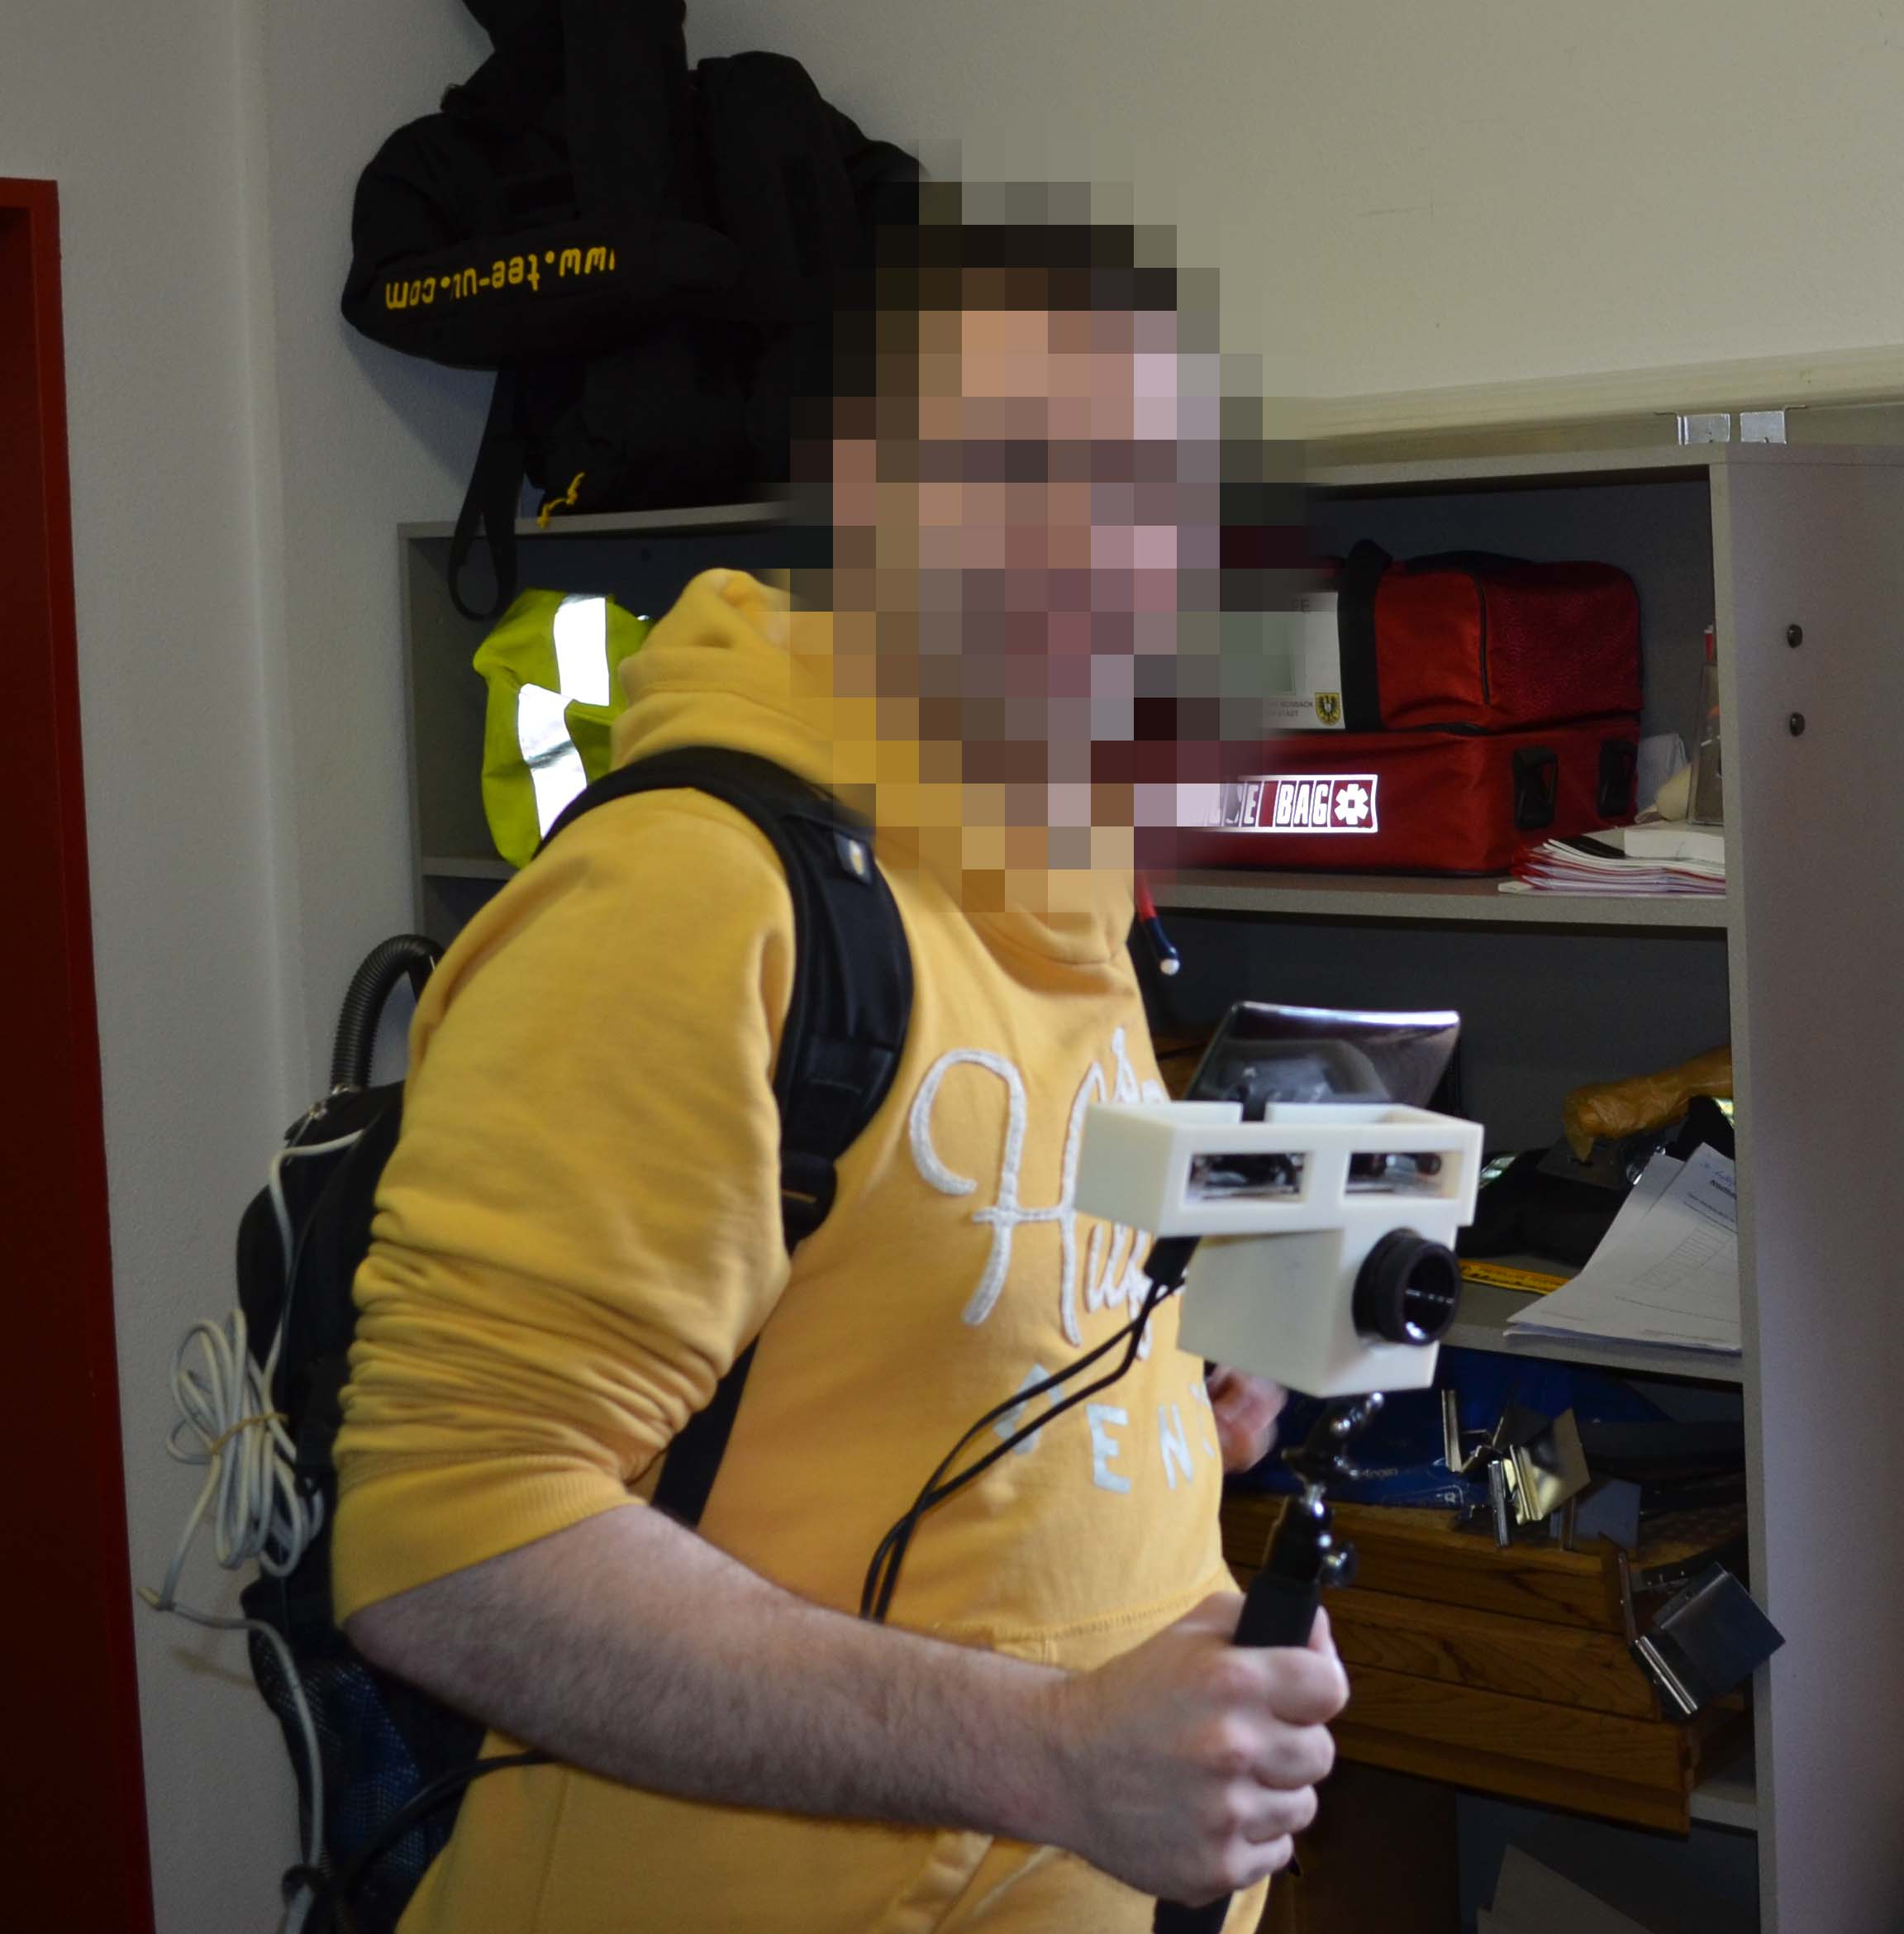
\includegraphics[width=\textwidth]{Spezi/handheld.jpg}}{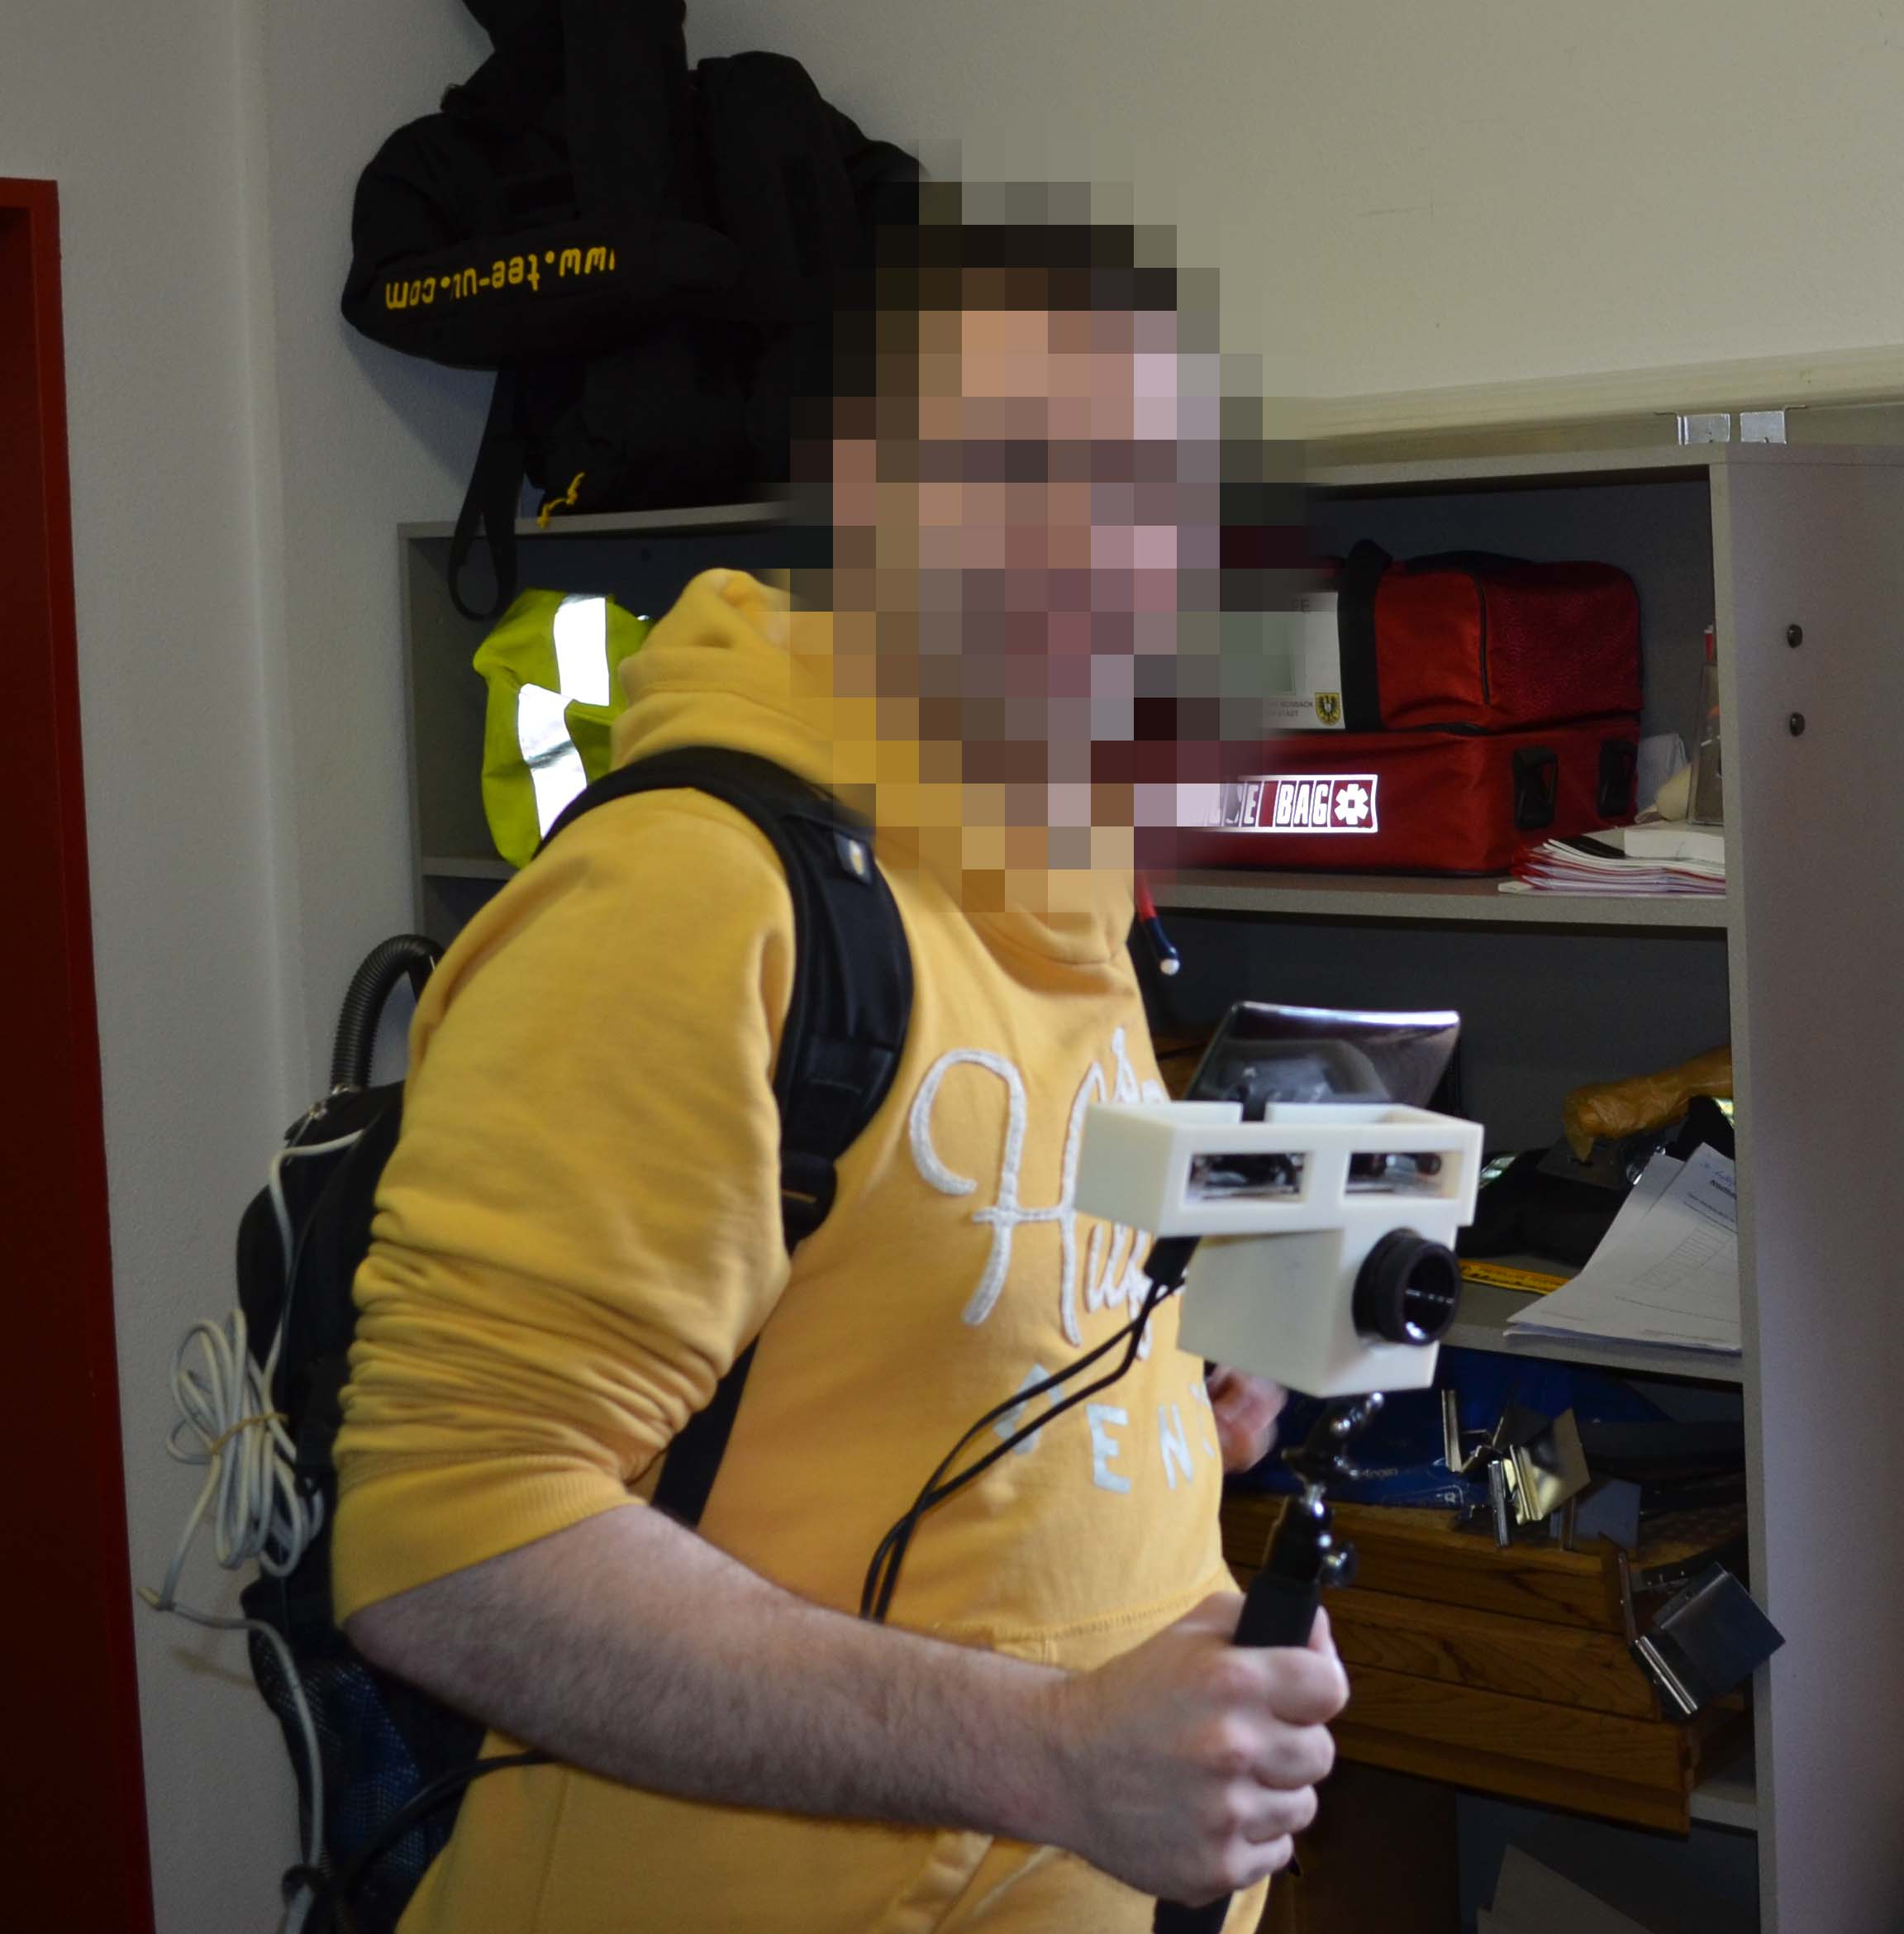
\includegraphics[width=\textwidth]{Spezi/handheld.png}}
		\caption{Handheld Prototyp}
		\label{fig:spezi_halterung_hand}
	\end{subfigure}
	~
	\begin{subfigure}[t]{0.45\textwidth}
		\centering
		\ifthenelse{\boolean{jpg}}{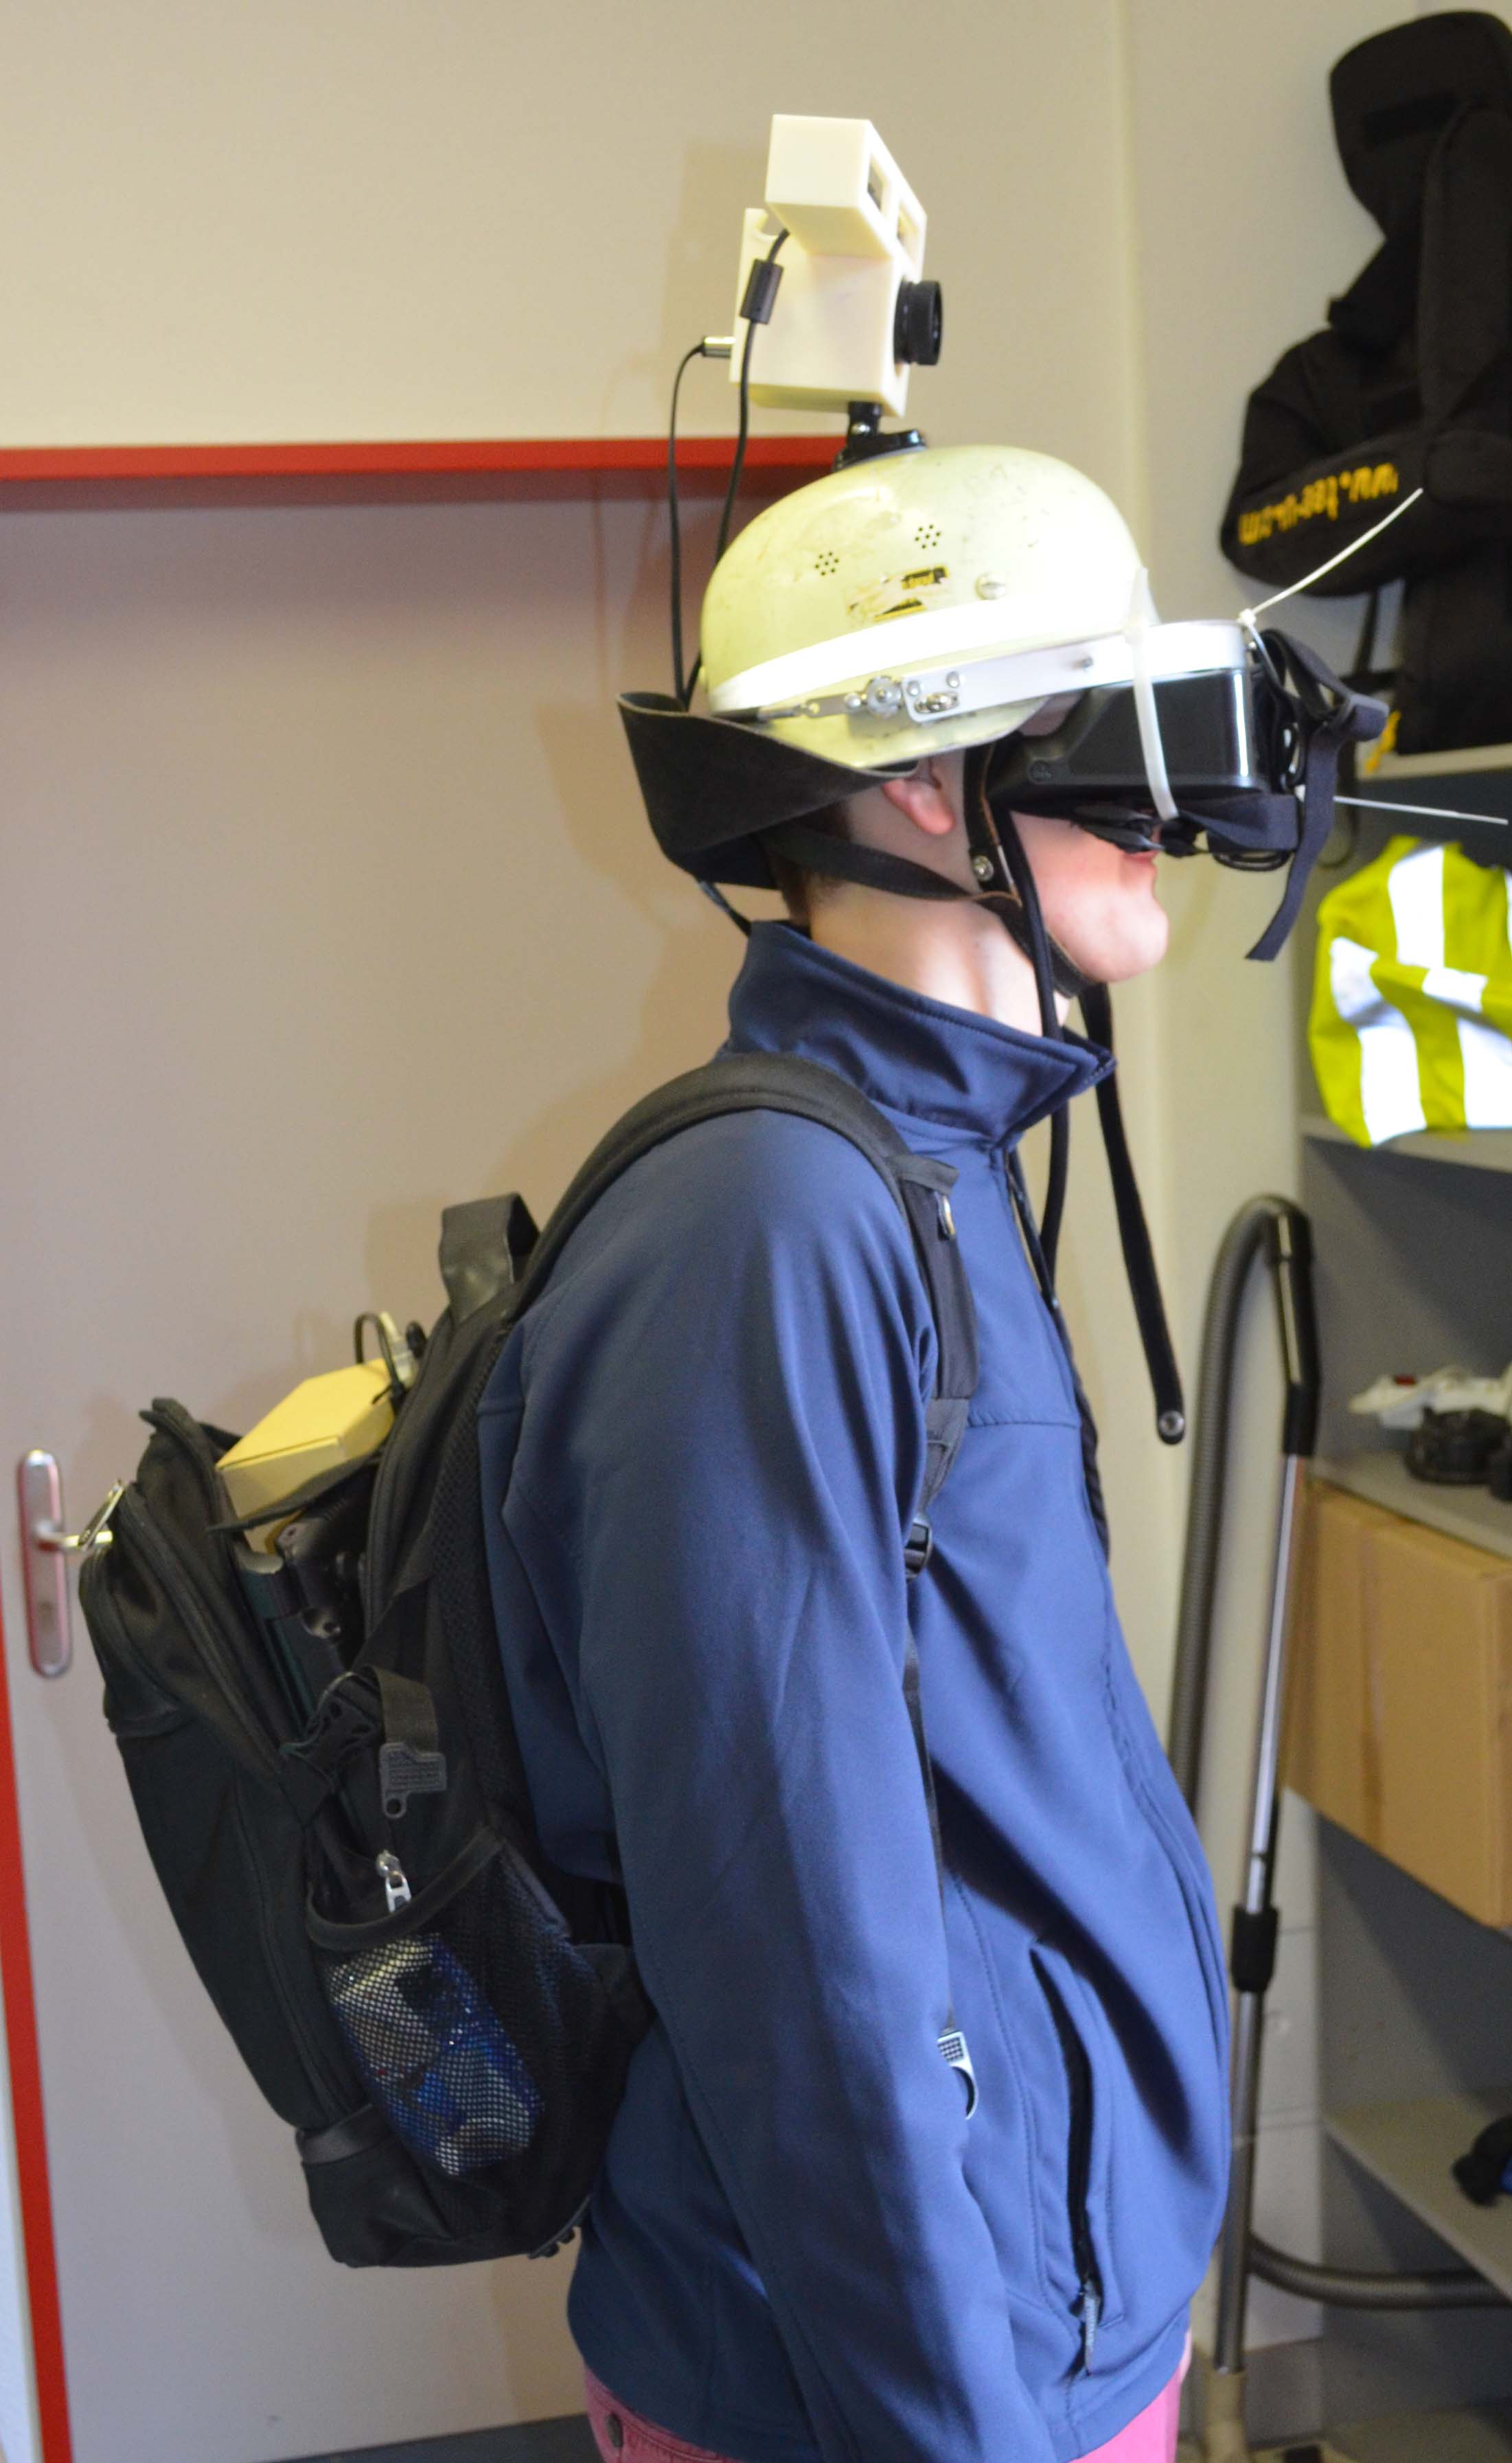
\includegraphics[scale=0.25]{Spezi/hmd.jpg}}{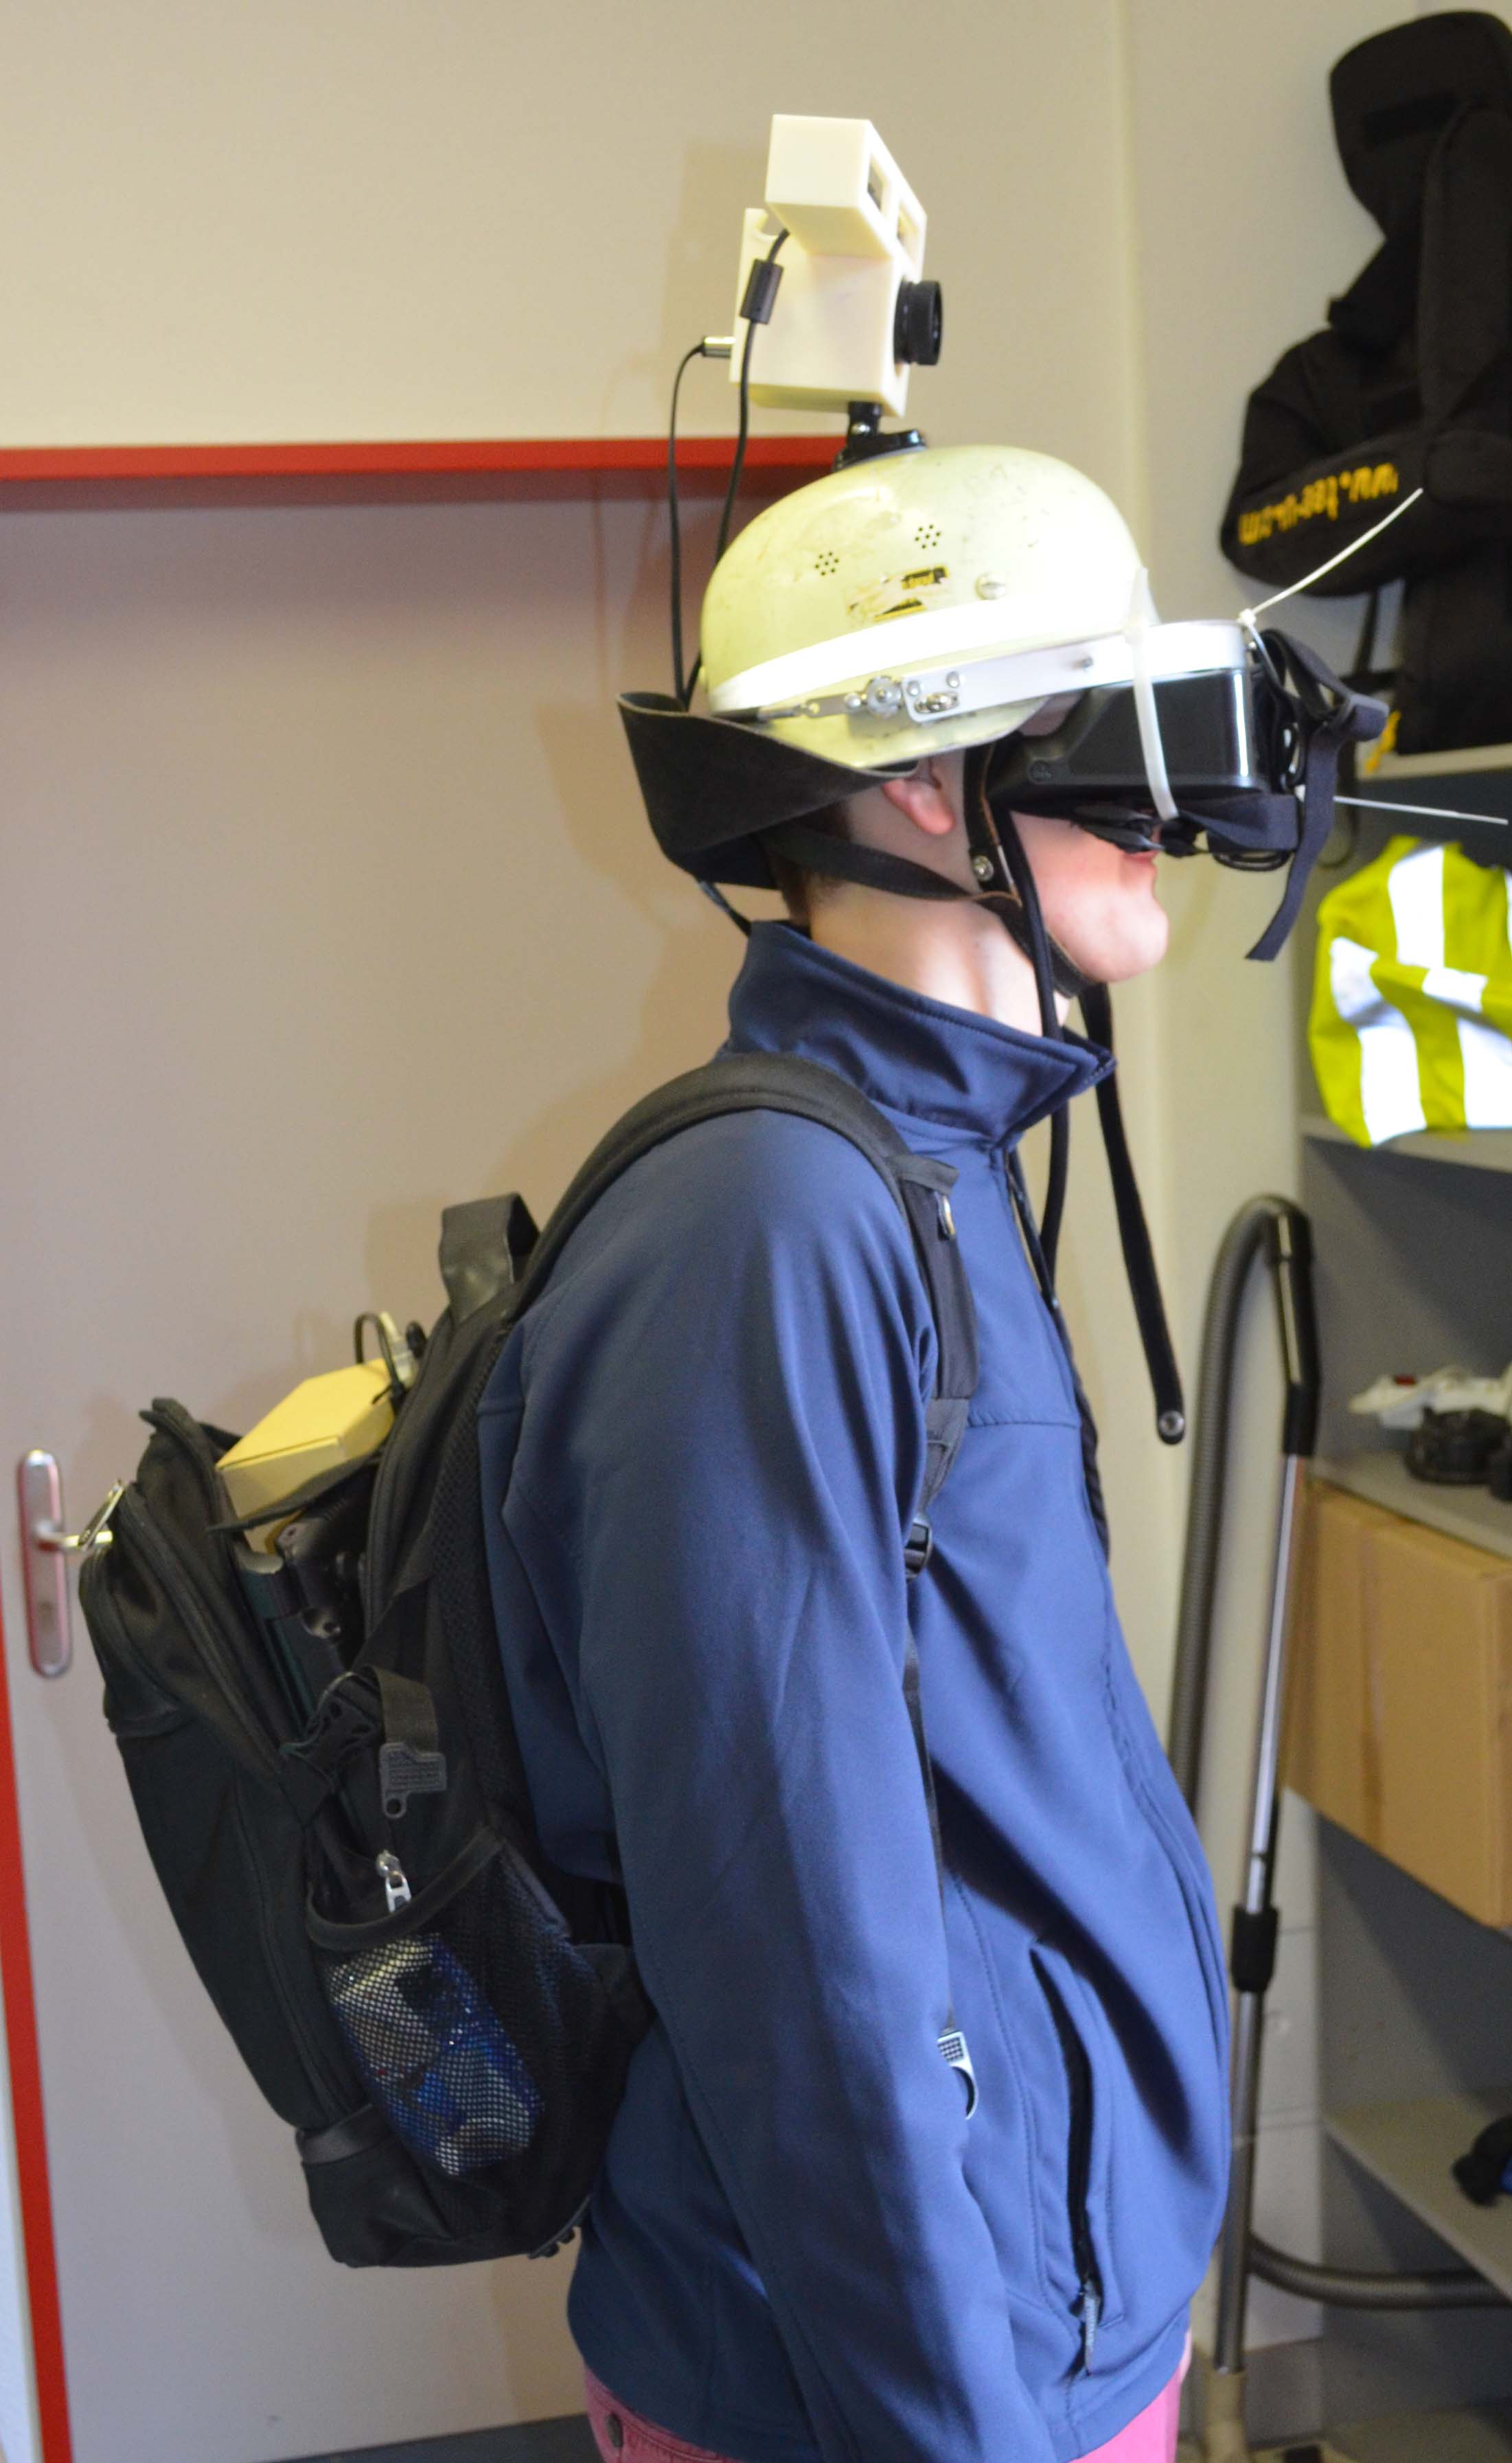
\includegraphics[scale=0.25]{Spezi/hmd.png}}
		\caption{Prototyp in Kombination mit einem Head Mounted Display}
		\label{fig:spezi_halterung_hmd}
	\end{subfigure}
	\caption{Halterungsaufbau}
	\label{fig:spezi_halterung}
\end{figure}

Die Wärmebildkamera und der \hyperlink{tab:tiefe}{Tiefenbild}sensor werden in einer gemeinsamen Halterung montiert.
Diese Halterung verfügt über ein Gewinde, welches eine Montage auf einem Standard GoPro-Handstativ ermöglicht.
Der Benutzer trägt die Halterung, über diesen Stick, per Hand.
Zusätzlich existiert die Möglichkeit, die Halterung an einem Feuerwehrhelm zu befestigen.

Die Programmsteuerung erfolgt über eine Maus oder ein mausähnliches Gerät, welches \ggf an der Halterung montiert ist.
Dabei werden lediglich die Maustasten zum Steuern benötigt.

Es sind zwei Ausgabemöglichkeiten vorgesehen, welche sich in ihrer Funktionalität nicht unterscheiden:
Erstere sieht so aus, dass der Benutzer eine Augmented Reality Brille (\meta) auf hat, welche am Laptop angeschlossen ist.
Hierbei kann der Benutzer über die AR Brille die verschiedenen Ausgabemethoden, wie Wärmebild, \hyperlink{tab:tiefe}{Tiefenbild} und beide fusioniert, direkt vor seinem Auge sehen.
Die zweite Variante funktioniert ähnlich wie die Erste.
Hierbei trägt der Benutzer ein mobiles Ausgabegerät (in unserem Fall ein Smartphone), welches \ggf sichtbar am Rücken der Halterung angebracht ist.
Das Ausgabegerät muss dafür im selben WLAN-Netz wie der Laptop sein.

Die GUI-Skizzen aus \cref{fig:spezi_mockup} geben einen Ausblick auf die anzustrebenden Ausgabemöglichkeiten:
\begin{figure}[t]
	\centering
	\begin{subfigure}[t]{0.45\textwidth}
		\centering
		\ifthenelse{\boolean{jpg}}{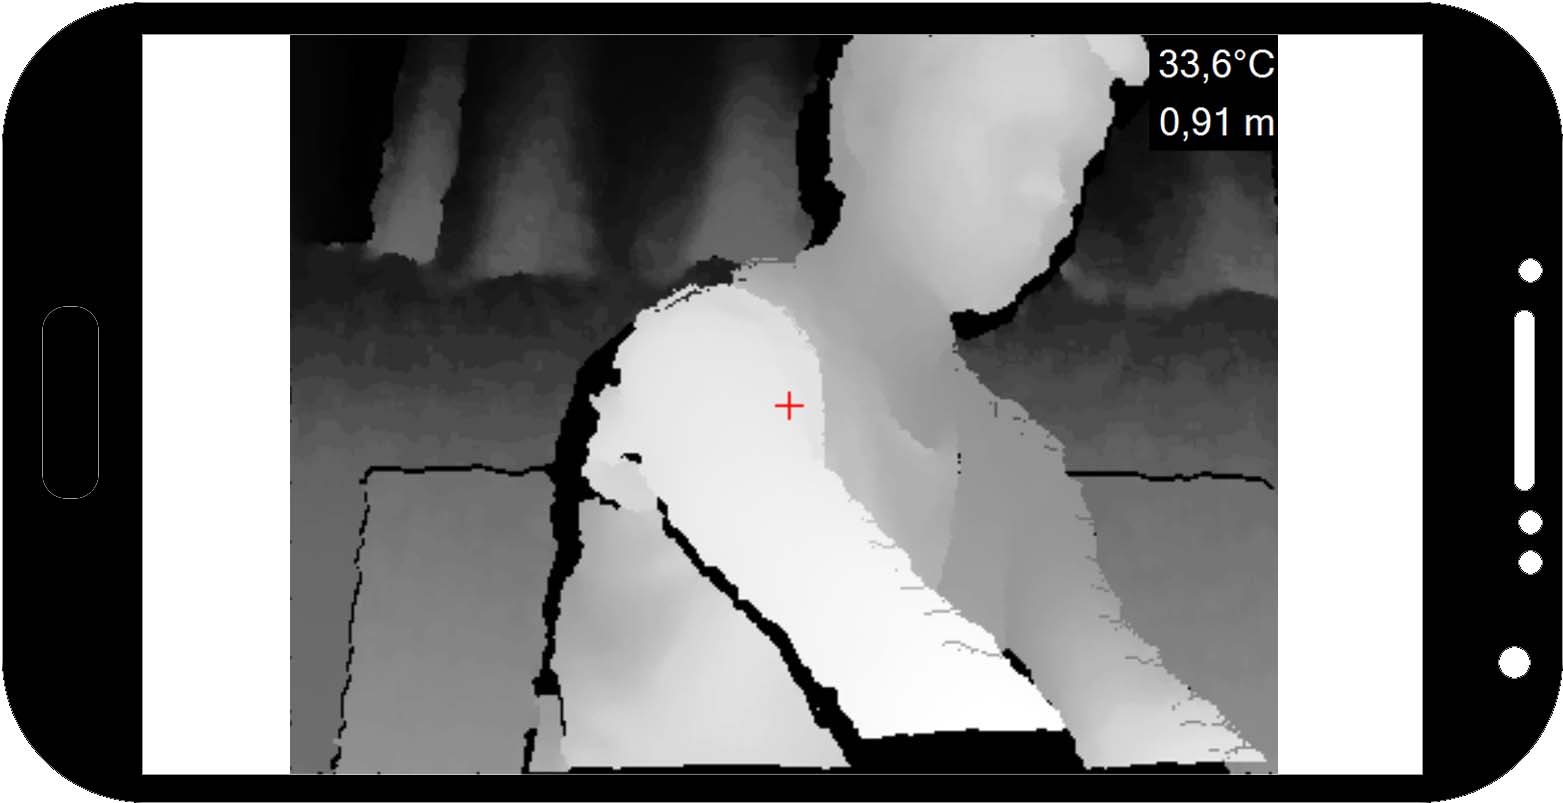
\includegraphics[width=\textwidth]{Spezi/depth_phone_mockup.jpg}}{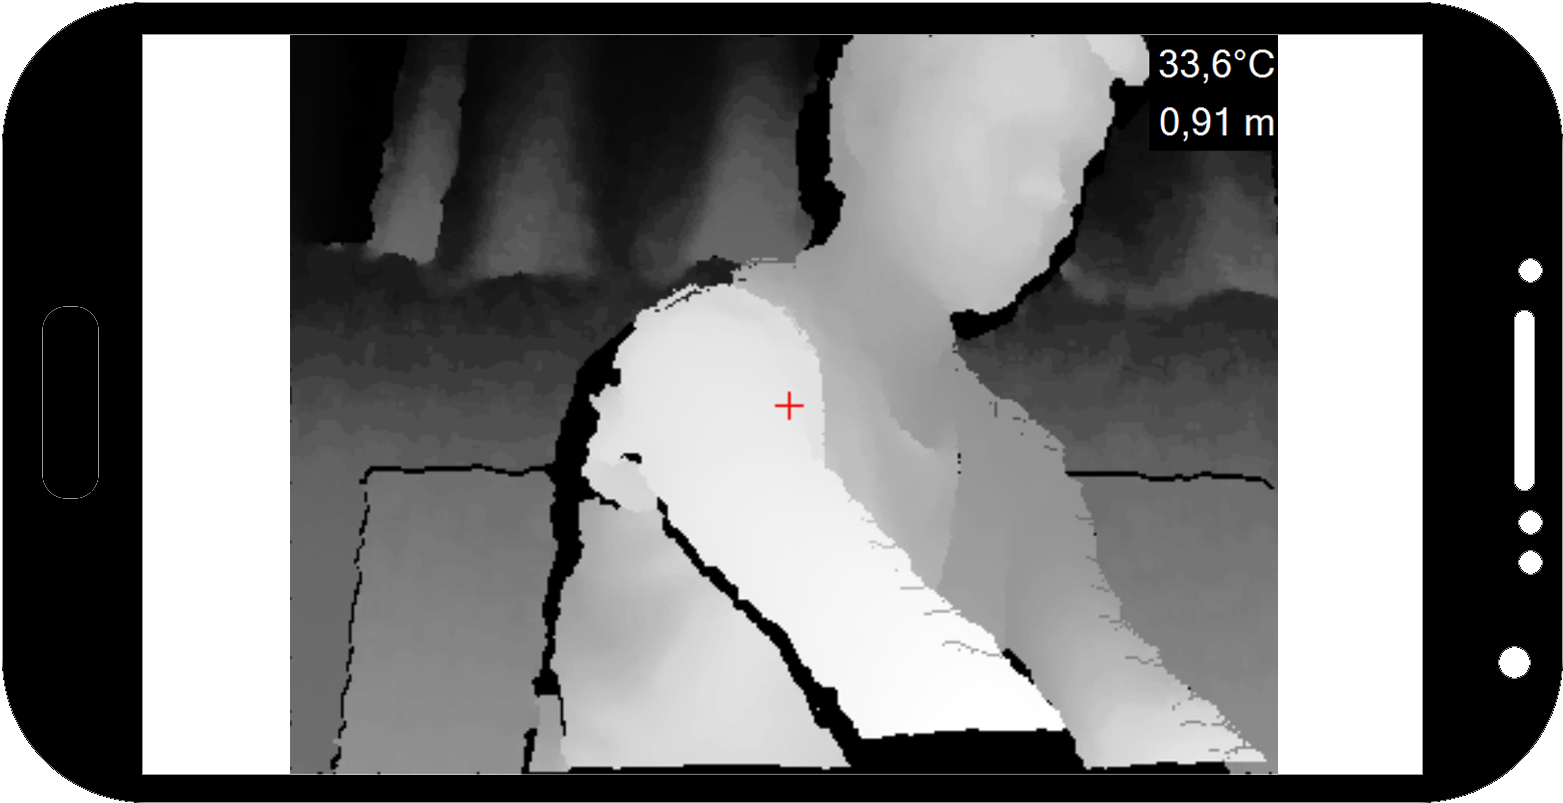
\includegraphics[width=\textwidth]{Spezi/depth_phone_mockup.png}}
		\caption{\hyperlink{tab:tiefe}{Tiefenbild}ausgabe auf mobilen Anzeigegerät}
		\label{fig:spezi_deepth_mockup}
	\end{subfigure}
	~
	\begin{subfigure}[t]{0.45\textwidth}
		\centering
		\ifthenelse{\boolean{jpg}}{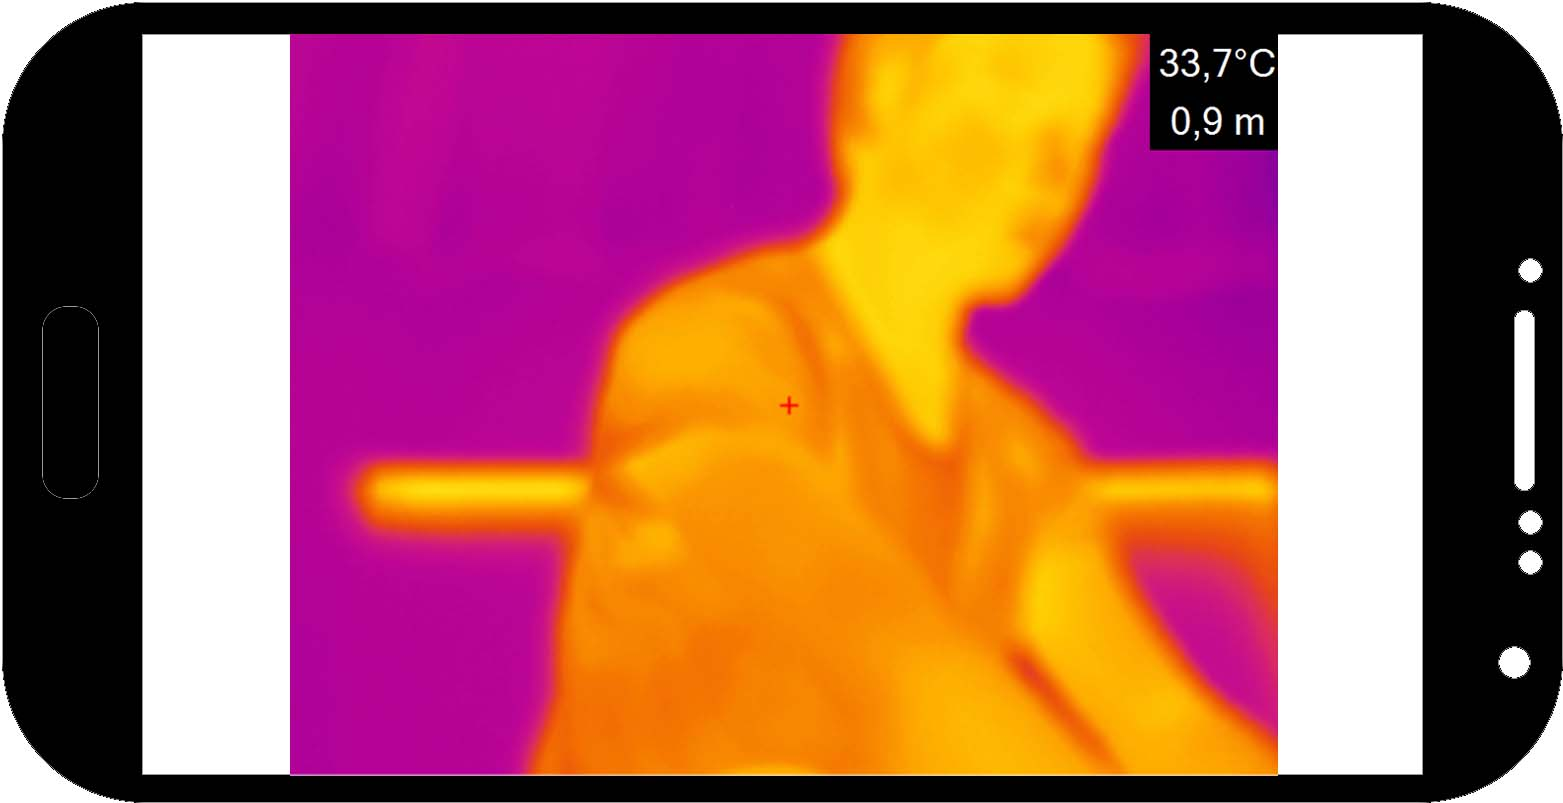
\includegraphics[width=\textwidth]{Spezi/heat_phone_mockup.jpg}}{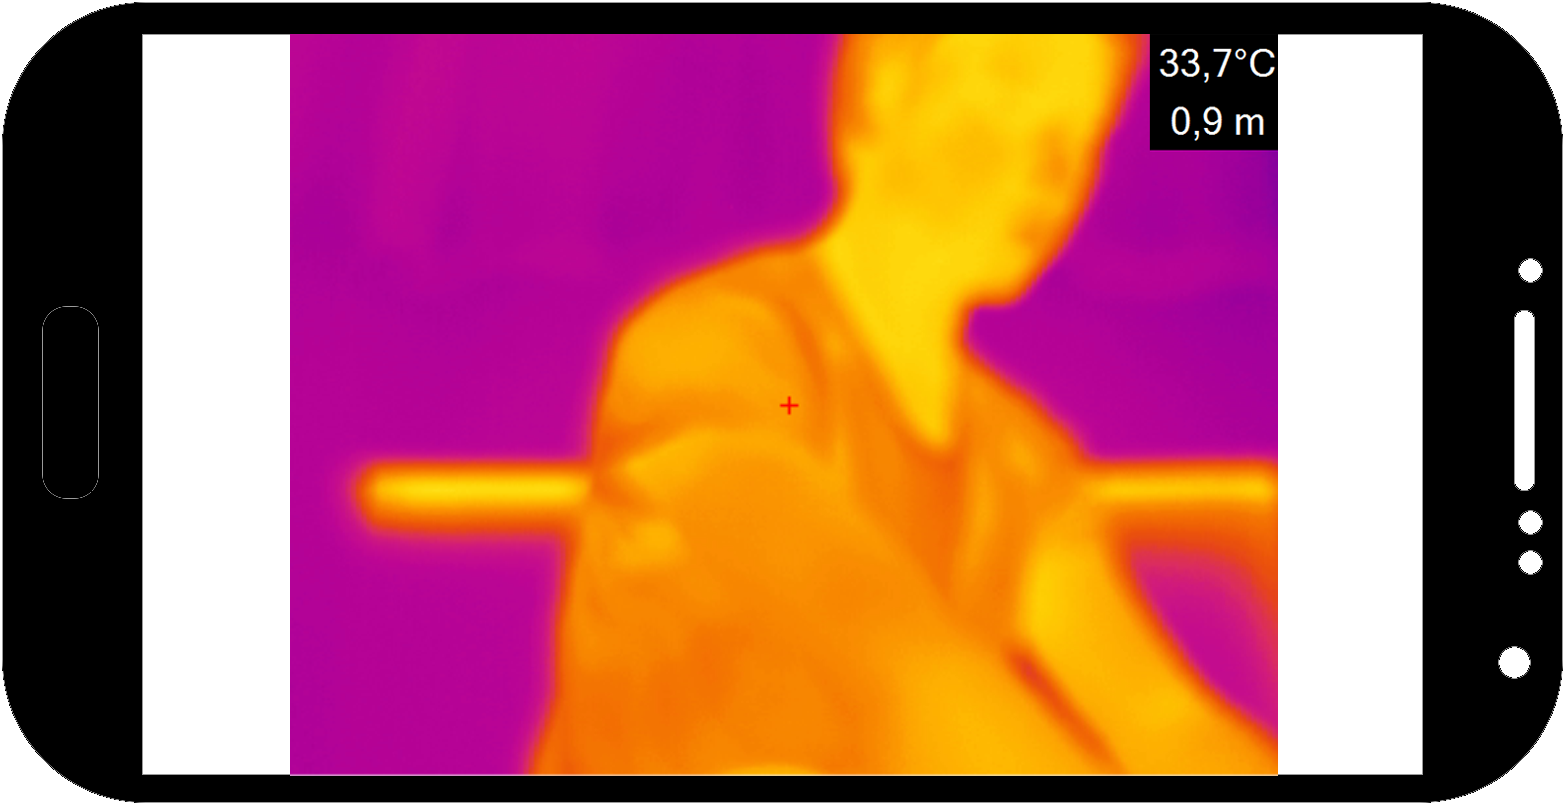
\includegraphics[width=\textwidth]{Spezi/heat_phone_mockup.png}}
		\caption{Wärmebildausgabe auf mobilen Anzeigegerät}
		\label{fig:spezi_heat_mockup}
	\end{subfigure}
	~
	\begin{subfigure}[t]{0.45\textwidth}
		\centering
		\ifthenelse{\boolean{jpg}}{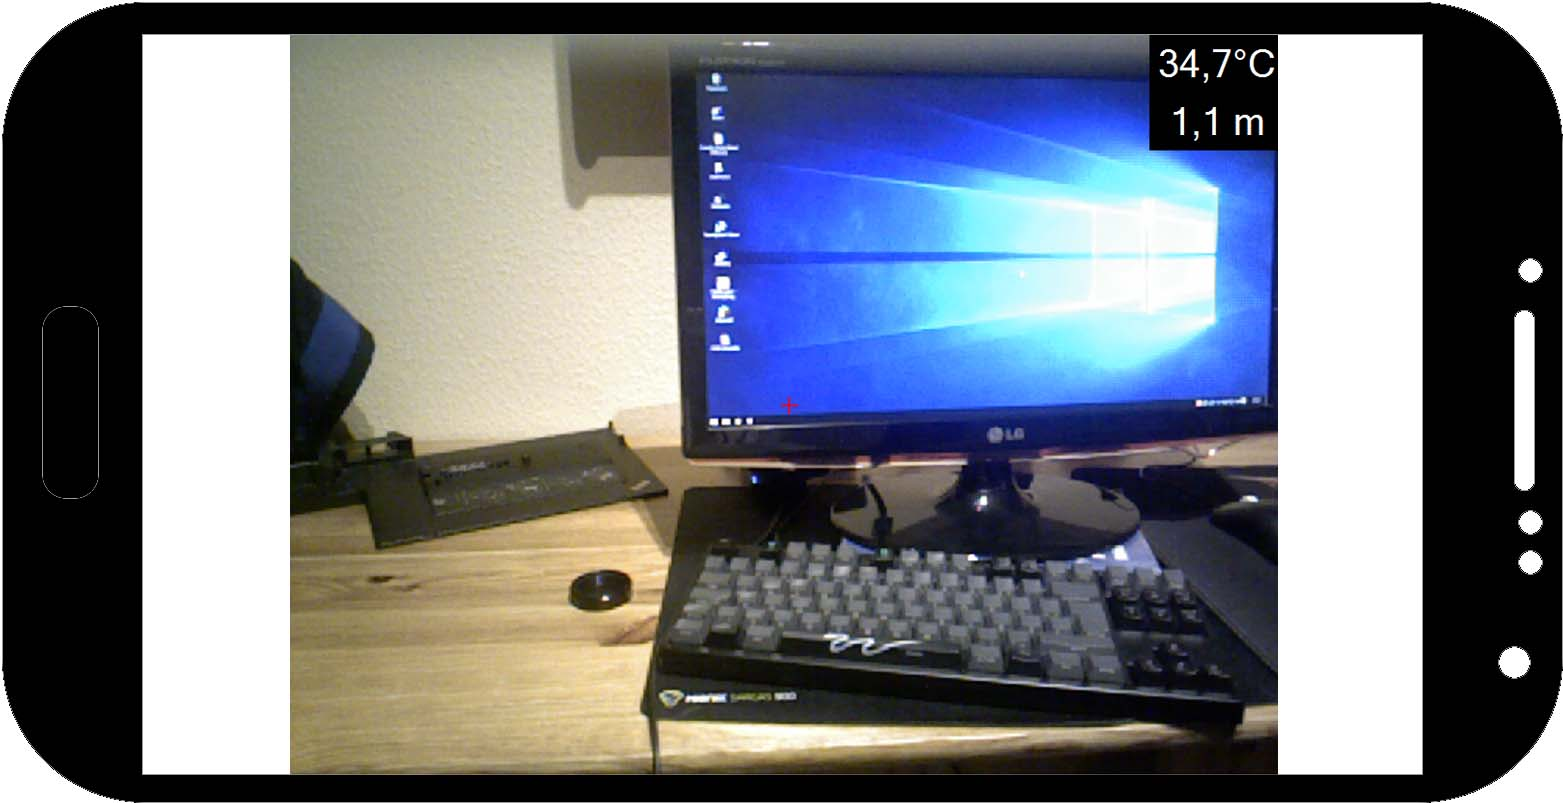
\includegraphics[width=\textwidth]{Spezi/rgb_phone_mockup.jpg}}{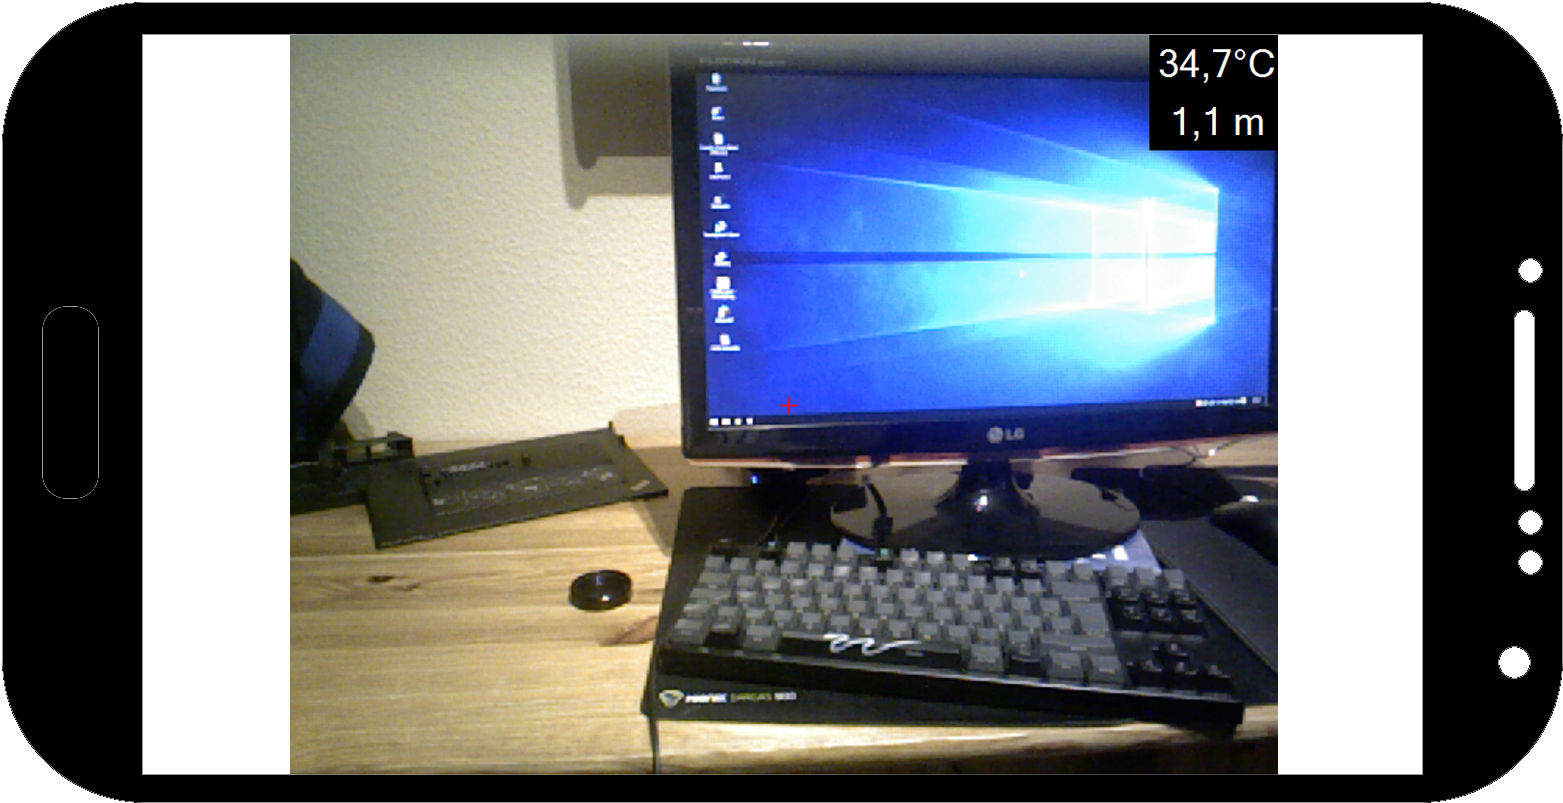
\includegraphics[width=\textwidth]{Spezi/rgb_phone_mockup.png}}
		\caption{RBG-Bildausgabe auf mobilen Anzeigegerät}
		\label{fig:spezi_rgb_mockup}
	\end{subfigure}
	~
	\begin{subfigure}[t]{0.45\textwidth}
		\centering
		\ifthenelse{\boolean{jpg}}{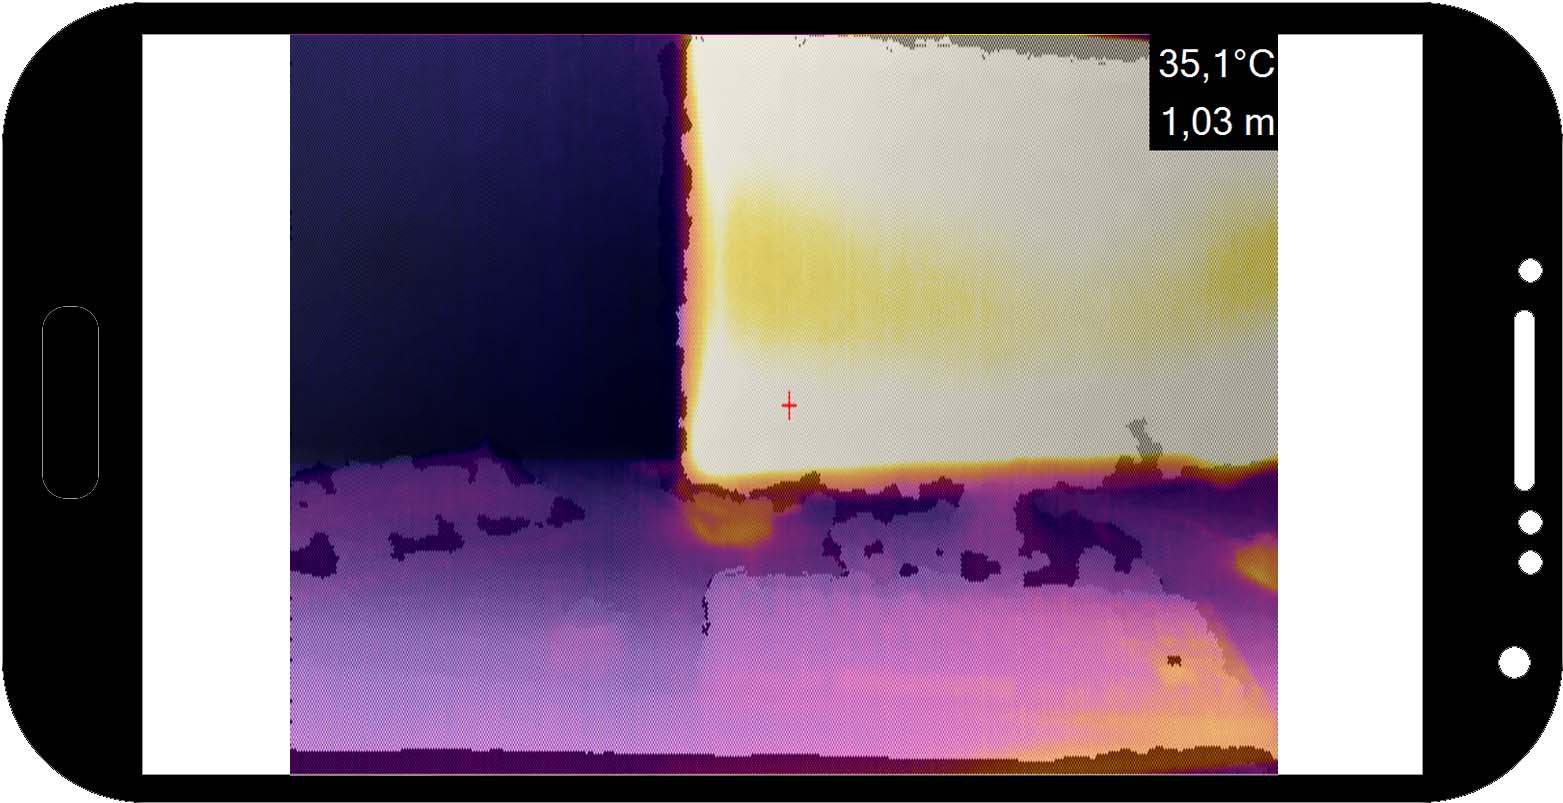
\includegraphics[width=\textwidth]{Spezi/fus_phone_mockup.jpg}}{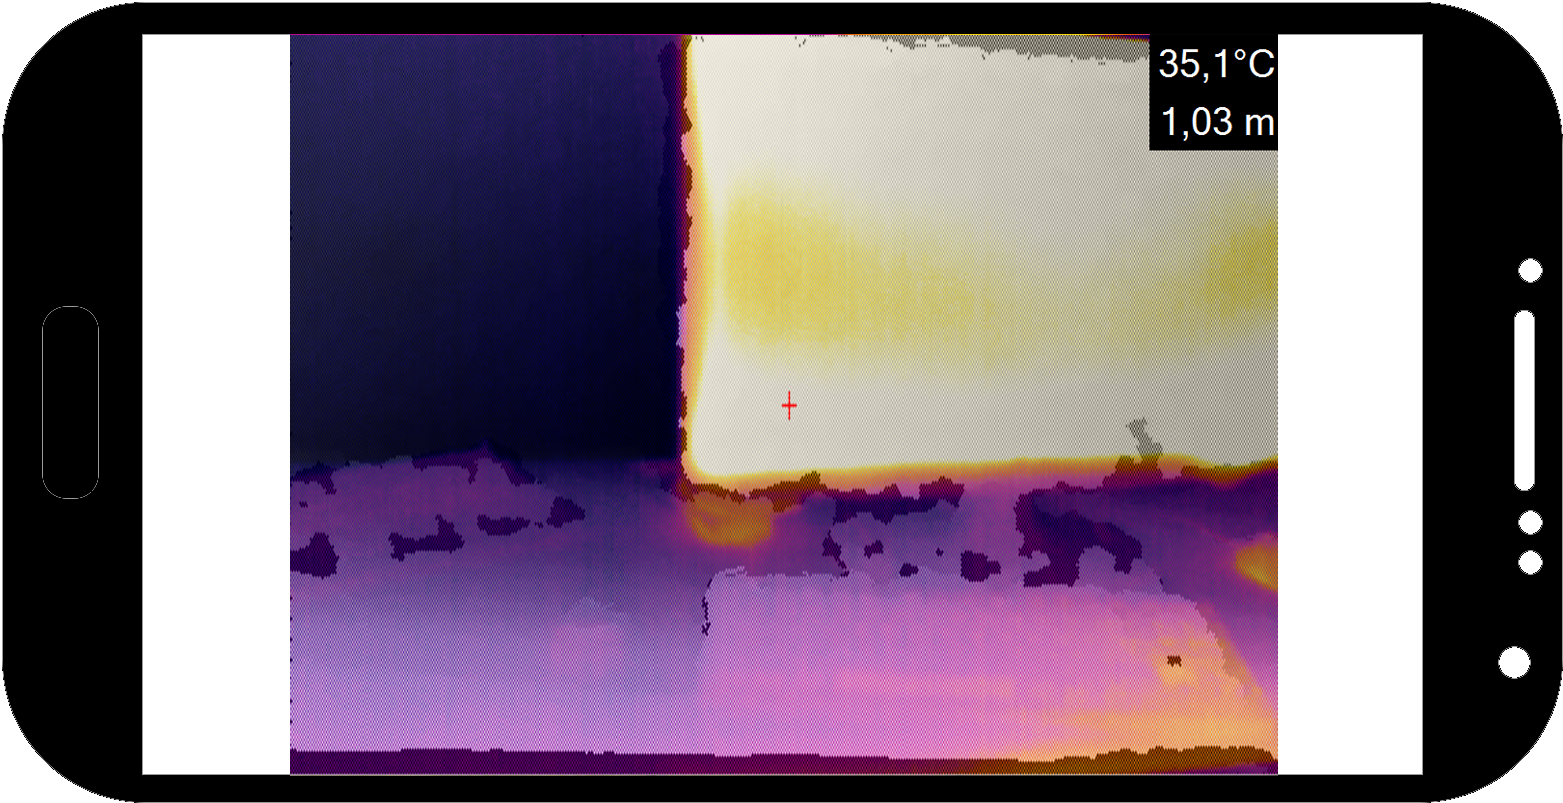
\includegraphics[width=\textwidth]{Spezi/fus_phone_mockup.png}}
		\caption{Erstellte Fusionsausgabe auf mobilen Anzeigegerät}
		\label{fig:spezi_fus_mockup}
	\end{subfigure}
	\caption{Mock-Ups der Ausgabe auf einem mobilen Anzeigegerät}
	\label{fig:spezi_mockup}
\end{figure}

\section{Anwendungsfälle}
\label{chap:spezi_usecases}

\subsection{Anwendungsfalldiagramm}
\begin{figure}[H]
	\centering
	\ifthenelse{\boolean{jpg}}{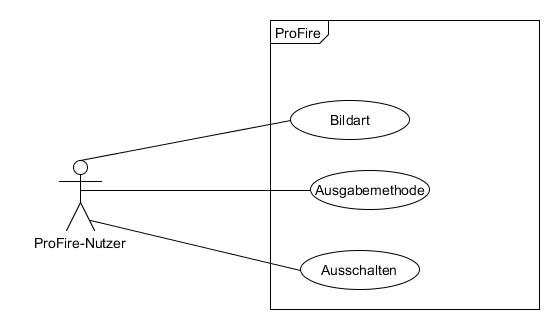
\includegraphics[width=0.8\textwidth]{Spezi/profire.jpg}}{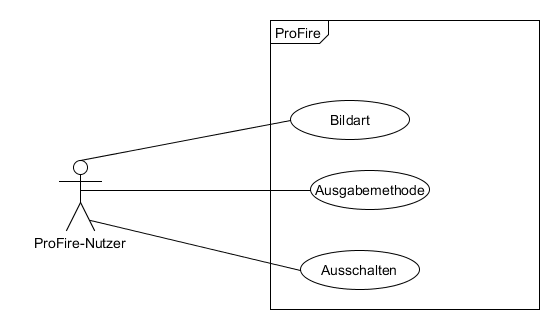
\includegraphics[width=0.8\textwidth]{Spezi/profire.png}}
	\caption{Zeigt die Funktionen von \profire}
	\label{fig:spezi_profire}
\end{figure}
\begin{figure}[H]
	\centering
	\ifthenelse{\boolean{jpg}}{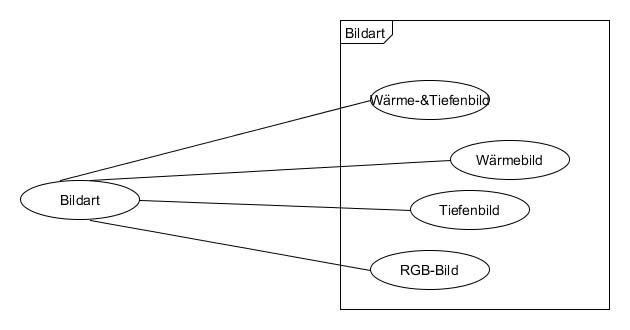
\includegraphics[width=0.8\textwidth]{Spezi/pic.jpg}}{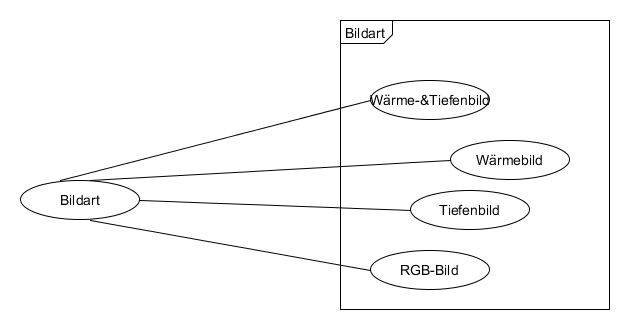
\includegraphics[width=0.8\textwidth]{Spezi/pic.png}}
	\caption{Zeigt die genauen Funktionen von Bildart}
	\label{fig:spezi_pic}
\end{figure}
\begin{figure}[H]
	\centering
	\ifthenelse{\boolean{jpg}}{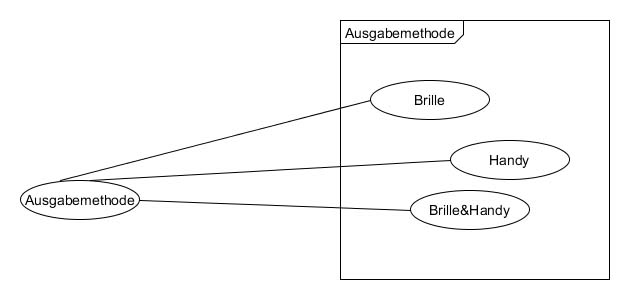
\includegraphics[width=0.8\textwidth]{Spezi/output.jpg}}{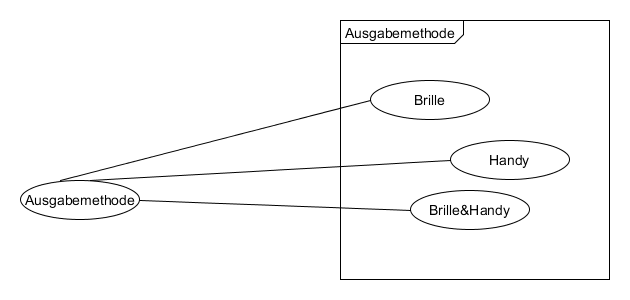
\includegraphics[width=0.8\textwidth]{Spezi/output.png}}
	\caption{Zeigt die genauen Funktionen von Ausgabemethode}
	\label{fig:spezi_output}
\end{figure}

\subsection{Beschreibung der Anwendungsfälle}
In den folgenden Anwendungsfälle wird davon ausgegangen, dass sowohl die Brille aus auch das mobile Anzeigegerät zur Bildausgabe genutzt wird.

\subsubsection{Das Tiefebild anzeigen}
\begin{center}
	\begin{longtable}{| p{3cm} | p{12cm} |}
		\hline
		\goal & Der Nutzer kann das \hyperlink{tab:tiefe}{Tiefenbild} sehen. \\ \hline
		
		\precondition & \begin{itemize}
			\item Die \hyperlink{tab:anwendung}{Software} wurde ordnungsgemäß gestartet.
			\item Die \hyperlink{tab:anwendung}{Software} zeigt nicht das \hyperlink{tab:tiefe}{Tiefenbild} an.
		\end{itemize} \\ \hline
		
		\postcondition & \begin{itemize}
			\item Das \hyperlink{tab:tiefe}{Tiefenbild} wird auf der Brille und auf dem mobilen Anzeigegerät angezeigt.
		\end{itemize} \\ \hline
		
		\postexception & --- \\ \hline
		
		\flow & \begin{enumerate}
			\item Der Nutzer betätigt den Linksklick der Maus.
			\item Es werden für jeden Klick nacheinander die verschiedenen Bildmodi angezeigt.
			\item Der Nutzer betätigt den Linksklick der Maus bis das \hyperlink{tab:tiefe}{Tiefenbild} angezeigt wird.
			\item Das \hyperlink{tab:tiefe}{Tiefenbild} wird angezeigt.			
		\end{enumerate} \\ \hline
		
		\exception & --- \\ \hline
		
		\player & Der Nutzer \\
		\hline
	\end{longtable}
\end{center}

\subsubsection{Das Wärmebild anzeigen}
\begin{center}
	\begin{longtable}{| p{3cm} | p{12cm} |}
		\hline
		\goal & Der Nutzer kann das Wärmebild sehen. \\ \hline
		
		\precondition & \begin{itemize}
			\item Die \hyperlink{tab:anwendung}{Software} wurde ordnungsgemäß gestartet.
			\item Die \hyperlink{tab:anwendung}{Software} zeigt nicht das Wärmebild an.
		\end{itemize} \\ \hline
		
		\postcondition & \begin{itemize}
			\item Das Wärmebild wird auf der Brille und auf dem mobilen Anzeigegerät angezeigt.
		\end{itemize} \\ \hline
		
		\postexception & --- \\ \hline
		
		\flow & \begin{enumerate}
			\item Der Nutzer betätigt den Linksklick der Maus.
			\item Es werden für jeden Klick nacheinander die verschiedenen Bildmodi angezeigt.
			\item Der Nutzer betätigt den Linksklick der Maus bis das Wärmebild angezeigt wird.
			\item Das Wärmebild wird angezeigt.			
		\end{enumerate} \\ \hline
		
		\exception & --- \\ \hline
		
		\player & Der Nutzer \\
		\hline
	\end{longtable}
\end{center}

\subsubsection{Das verbesserte Wärmebild anzeigen}
\begin{center}
	\begin{longtable}{| p{3cm} | p{12cm} |}
		\hline
		\goal & Der Nutzer kann das verbesserte Wärmebild sehen. \\ \hline
		
		\precondition & \begin{itemize}
			\item Die \hyperlink{tab:anwendung}{Software} wurde ordnungsgemäß gestartet.
			\item Die \hyperlink{tab:anwendung}{Software} zeigt nicht das verbesserte Wärmebild an.
		\end{itemize} \\ \hline
		
		\postcondition & \begin{itemize}
			\item Das verbesserte Wärmebild wird auf der Brille und auf dem mobilen Anzeigegerät angezeigt.
		\end{itemize} \\ \hline
		
		\postexception & --- \\ \hline
		
		\flow & \begin{enumerate}
			\item Der Nutzer betätigt den Linksklick der Maus.
			\item Es werden für jeden Klick nacheinander die verschiedenen Bildmodi angezeigt.
			\item Der Nutzer betätigt den Linksklick der Maus bis das verbesserte Wärmebild angezeigt wird.
			\item Das verbesserte Wärmebild wird angezeigt.			
		\end{enumerate} \\ \hline
		
		\exception & --- \\ \hline
		
		\player & Der Nutzer \\
		\hline
	\end{longtable}
\end{center}

\subsubsection{Das RGB-Bild anzeigen}
\begin{center}
	\begin{longtable}{| p{3cm} | p{12cm} |}
		\hline
		\goal & Der Nutzer kann das RGB-Bild sehen. \\ \hline
		
		\precondition & \begin{itemize}
			\item Die \hyperlink{tab:anwendung}{Software} wurde ordnungsgemäß gestartet.
			\item Die \hyperlink{tab:anwendung}{Software} zeigt nicht das RGB-Bild an.
		\end{itemize} \\ \hline
		
		\postcondition & \begin{itemize}
			\item Das RGB-Bild wird auf der Brille und auf dem mobilen Anzeigegerät angezeigt.
		\end{itemize} \\ \hline
		
		\postexception & --- \\ \hline
		
		\flow & \begin{enumerate}
			\item Der Nutzer betätigt den Linksklick der Maus.
			\item Es werden für jeden Klick nacheinander die verschiedenen Bildmodi angezeigt.
			\item Der Nutzer betätigt den Linksklick der Maus bis das RGB-Bild angezeigt wird.
			\item Das RGB-Bild wird angezeigt.			
		\end{enumerate} \\ \hline
		
		\exception & --- \\ \hline
		
		\player & Der Nutzer \\
		\hline
	\end{longtable}
\end{center}

\subsubsection{Ausgabe auf der Brille deaktivieren}
\begin{center}
	\begin{longtable}{| p{3cm} | p{12cm} |}
		\hline
		\goal & Es findet keine Ausgabe auf der Brille statt. \\ \hline
		
		\precondition & \begin{itemize}
			\item Die \hyperlink{tab:anwendung}{Software} wurde ordnungsgemäß gestartet.
			\item Das Bild wird auf der Brille und dem mobilen Anzeigegerät angezeigt.
		\end{itemize} \\ \hline
		
		\postcondition & \begin{itemize}
			\item Der gleiche Bildmodus wird nur auf dem mobilen Anzeigegerät angezeigt.
		\end{itemize} \\ \hline
		
		\postexception & --- \\ \hline
		
		\flow & \begin{enumerate}
			\item Der Nutzer betätigt den Rechtsklick der Maus.
			\item Auf der Brille wird angezeigt ein schwarzes Overlay angezeigt, um eine Transparenz zu simulieren.			
		\end{enumerate} \\ \hline
		
		\exception & --- \\ \hline
		
		\player & Der Nutzer \\
		\hline
	\end{longtable}
\end{center}

\subsubsection{Ausgabe auf der Brille aktivieren}
\begin{center}
	\begin{longtable}{| p{3cm} | p{12cm} |}
		\hline
		\goal & Es findet eine Ausgabe auf der Brille und dem mobilen Anzeigegerät statt. \\ \hline
		
		\precondition & \begin{itemize}
			\item Die \hyperlink{tab:anwendung}{Software} wurde ordnungsgemäß gestartet.
			\item Das Bild wird nur auf dem mobilen Anzeigegerät angezeigt.
		\end{itemize} \\ \hline
		
		\postcondition & \begin{itemize}
			\item Der gleiche Bildmodus wird auf der Brille und dem mobilen Anzeigegerät angezeigt.
		\end{itemize} \\ \hline
		
		\postexception & --- \\ \hline
		
		\flow & \begin{enumerate}
			\item Der Nutzer betätigt den Rechtsklick der Maus.
			\item Auf der Brille wird der ausgewählte Bildmodus angezeigt.
		\end{enumerate} \\ \hline
		
		\exception & --- \\ \hline
		
		\player & Der Nutzer \\
		\hline
	\end{longtable}
\end{center}

\subsubsection{Das Programm starten}
\begin{center}
	\begin{longtable}{| p{3cm} | p{12cm} |}
		\hline
		\goal & Das Programm läuft und der Nutzer kann das Programm benutzen. \\ \hline
		
		\precondition & \begin{itemize}
			\item Der PC, auf dem die \hyperlink{tab:anwendung}{Software} ausgeführt werden soll, läuft.
			\item Das Setup ist fertig aufgebaut
			\begin{itemize}
				\item Die Brille ist eingeschaltet.
				\item Alle Kabel sind eingesteckt.
				\item Das Gerät für die Mobile Ausgabe ist mit dem PC verbunden.
			\end{itemize}
			\item Der Nutzer hat den Ordner geöffnet, indem sich die Anwendung zum Starten des Programms befindet.
		\end{itemize} \\ \hline
		
		\postcondition & \begin{itemize}
			\item Der Benutzer kann das Programm bedienen.
			\item Das verbesserte Wärmebild wird auf der Brille und auf dem mobilen Anzeigegerät angezeigt
		\end{itemize} \\ \hline
		
		\postexception & --- \\ \hline
		
		\flow & \begin{enumerate}
			\item Der Nutzer betätigt einen Doppelklick auf die Anwendung, die das Programm startet.
			\item Das Programm startet und es wird ein schwarzer Bildschirm angezeigt.
			\item Der Nutzer betätigt den Linksklick der Maus.
			\item Das verbesserte Wärmebild wird angezeigt.			
		\end{enumerate} \\ \hline
		
		\exception & --- \\ \hline
		
		\player & Der Nutzer \\
		\hline
	\end{longtable}
\end{center}

\subsubsection{Das Programm beenden}
\begin{center}
	\begin{longtable}{| p{3cm} | p{12cm} |}
		\hline
		\goal & Das Programm ist geschlossen. \\ \hline
		
		\precondition & \begin{itemize}
			\item Das Programm läuft und einer der Bildmodi wird angezeigt.
		\end{itemize} \\ \hline
		
		\postcondition & \begin{itemize}
			\item Das Programm ist geschlossen.
			\item Der Nutzer hat den Ordner geöffnet, indem sich die Anwendung zum Starten des Programms befindet.
		\end{itemize} \\ \hline
		
		\postexception & --- \\ \hline
		
		\flow & \begin{enumerate}
			\item Der Nutzer drückt die \enquote{ESC}-Taste.
			\item Das Programm schließt sich.
			\item Der Nutzer hat den Ordner geöffnet, indem sich die Anwendung zum Starten des Programms befindet.			
		\end{enumerate} \\ \hline
		
		\exception & --- \\ \hline
		
		\player & Der Nutzer \\
		\hline
	\end{longtable}
\end{center}

\subsubsection{Das Tiefebild anzeigen}
\begin{center}
	\begin{longtable}{| p{3cm} | p{12cm} |}
		\hline
		\goal & Der Nutzer kann das \hyperlink{tab:tiefe}{Tiefenbild} sehen. \\ \hline
		
		\precondition & \begin{itemize}
			\item Die \hyperlink{tab:anwendung}{Software} wurde ordnungsgemäß gestartet.
			\item Die \hyperlink{tab:anwendung}{Software} zeigt nicht das \hyperlink{tab:tiefe}{Tiefenbild} an.
		\end{itemize} \\ \hline
		
		\postcondition & \begin{itemize}
			\item Das \hyperlink{tab:tiefe}{Tiefenbild} wird auf der Brille und auf dem mobilen Anzeigegerät angezeigt.
		\end{itemize} \\ \hline
		
		\postexception & --- \\ \hline
		
		\flow & \begin{enumerate}
			\item Der Nutzer betätigt den Linksklick der Maus.
			\item Es werden für jeden Klick nacheinander die verschiedenen Bildmodi angezeigt.
			\item Der Nutzer betätigt den Linksklick der Maus bis das \hyperlink{tab:tiefe}{Tiefenbild} angezeigt wird.
			\item Das \hyperlink{tab:tiefe}{Tiefenbild} wird angezeigt.			
		\end{enumerate} \\ \hline
		
		\exception & --- \\ \hline
		
		\player & Der Nutzer \\
		\hline
	\end{longtable}
\end{center}

\section{Anhang}
\label{chap:spezi_append}

\subsection{Begriffslexikon}
\begin{center}
	\hypertarget{tab:tiefe}{}
	\begin{tabular}{| p{4cm} | p{11cm} |}
		\hline
		\term & Tiefe, Tiefenbild \\ \hline
		
		\intent & Darstellung der Distanz von Objekten durch unterschiedliche Farbabstufungen \\ \hline
		
		\bound & --- \\ \hline
		
		\validity & --- \\ \hline
		
		\identifier & --- \\ \hline
		
		\blur & --- \\ \hline
		
		\crossref & --- \\
		\hline
	\end{tabular}
\end{center}

\begin{center}
	\hypertarget{tab:sonne}{}
	\begin{tabular}{| p{4cm} | p{11cm} |}
		\hline
		\term & direktes Sonnenlicht  \\ \hline
		
		\intent & Sonnenlicht das direkt auf Objekte strahlt und zuvor nicht durch Glasfenster gefiltert wurde \\ \hline
		
		\bound & --- \\ \hline
		
		\validity & --- \\ \hline
		
		\identifier & --- \\ \hline
		
		\blur & --- \\ \hline
		
		\crossref & --- \\
		\hline
	\end{tabular}
\end{center}

\begin{center}
	\hypertarget{tab:strahlung}{}
	\begin{tabular}{| p{4cm} | p{11cm} |}
		\hline
		\term & Überstrahlung, abstrahlen \\ \hline
		
		\intent & Objekt, welches so heiß ist, sodass es die herumliegende Umgebung mit erwärmt \\ \hline
		
		\bound & --- \\ \hline
		
		\validity & --- \\ \hline
		
		\identifier & --- \\ \hline
		
		\blur & --- \\ \hline
		
		\crossref & --- \\
		\hline
	\end{tabular}
\end{center}

\begin{center}
	\hypertarget{tab:system}{}
	\begin{tabular}{| p{4cm} | p{11cm} |}
		\hline
		\term & System, Programm, \profire \\ \hline
		
		\intent & Das System ist die \hyperlink{tab:anwendung}{Software} wie sie in diesem Dokument spezifiziert ist, mit all ihren geplanten bzw. schon realisierten Funktionen. \\ \hline
		
		\bound & Der Begriff System ist insbesondere nicht gleich zu verstehen mit dem Begriff \hyperlink{tab:anwendung}{Anwendung}, auch wenn eine \hyperlink{tab:anwendung}{Anwendung} immer ein System ist. \\ \hline
		
		\validity & --- \\ \hline
		
		\identifier & --- \\ \hline
		
		\blur & --- \\ \hline
		
		\crossref & \hyperlink{tab:anwendung}{Anwendung} \\
		\hline
	\end{tabular}
\end{center}

\begin{center}
	\hypertarget{tab:anwendung}{}
	\begin{tabular}{| p{4cm} | p{11cm} |}
		\hline
		\term & Anwendung, Software \\ \hline
		
		\intent & Die Anwendung ist eine voll ausführbare Version des \hyperlink{tab:system}{System}. \\ \hline
		
		\bound & Entwicklungsprototypen oder Testversionen sind keine Anwendung \\ \hline
		
		\validity & Sobald die Anwendung stabil läuft ist sie eine gültige Anwendung. \\ \hline
		
		\identifier & Die Anwendung ist durch die Funktionen und durch die Versionsnummer gekennzeichnet. \\ \hline
		
		\blur & --- \\ \hline
		
		\crossref & \hyperlink{tab:system}{System} \\
		\hline
	\end{tabular}
	\label{tab:anwendung}
\end{center}

\section{Versionhistorie}
\label{chap:spezi_version}

\begin{description}
	\item [Version 0.1 (28.06.2015 )] Erstellung des Dokuments
	\item [Version 1.0 (7.07.2015)] Überarbeitung Setup
	\item [Version 1.1 (18.7.2015)] Genauere Spezifizierung der Nicht-funktionalen Anforderungen \& Programmsteuerung
	\item [Version 1.2 (3.3.2016)] Aktualisierung \& Korrektur des Dokuments
\end{description}
% !TeX spellcheck = de_DE

\chapter{Entwurf}
\label{chap:entwurf}

Während in der Spezifikation noch auf den zu erstellenden Prototypen eingegangen wurde, protokolliert der Entwurf die Designentscheidungen und Struktur der zu erstellenden Software.

\section{Einleitung}

\subsection{Zweck des Entwurfs}
Der Entwurf bietet den Entwicklern ein Grundgerüst, das als Orientierung der Software dienen soll.
Es werden alle grundlegenden Entscheidungen \bzgl der Struktur der Software festgehalten.
Hierbei werden das Gesamtsystem, sowie einzelne Komponenten detailliert mit Hilfe von UML-Diagrammen beschrieben.
Durch das Dokument soll auch den zukünftigen Software-Entwicklern die Wartung der Software erleichtert werden.

\subsection{Lesekreis des Entwurfs}
Folgende Personen gehören zum Leserkreis dieses Dokuments:
\begin{itemize}
	\item Der Kunde
	\item Das gesamte Entwicklerteam
	\item Die universitären Betreuer
\end{itemize}

\subsection{Überblick über das Entwurfsdokument}
Zunächst werde in Kapitel 2 die grundsätzliche Entwurfsentscheidungen beschrieben.

In Kapitel 3 werden die einzelnen Komponente detailliert beschrieben.

\subsection{Schreibweisen und Abkürzungen}
Paketnamen werden im Dokument \textbf{fett} hervorgehoben. Klassennamen werden \textit{kursiv} dargestellt.

Bei eventuell unklaren Fachbegriffen und Abkürzungen, ist im Begriffslexikon der Spezifikation \bzw der Spezifikation selbst eine Erklärung zu selbigen zu finden.

\subsection{Aufbau dieses Dokuments}
Zunächst sollen allgemeine Entwurfsentscheidungen, wie verwendete Entwurfs- und Architekturmuster erläutert werden.
Dies soll ein Überblick über die grundsätzliche Struktur und Vorgehensweise im Entwurf verschaffen.
Im darauffolgenden Kapitel werden die Komponenten mit ihren Paketen und Klassen detailliert beschrieben.

\subsection{Einschränkungen in der Technik}
Die Implementierung muss in C\# 5 erfolgen.
Zusätzlich müssen die SDKs der Kameras bestmöglich benutzt werden.

\section{Grundsätzliche Entwurfsentscheidungen}

\subsection{Entworfene Software und Anforderung an den Entwurf}
Die Software soll die Bilder einer Wärmebildkamera oder Tiefenbildkamera anzeigen und in beiden Bildern soll zusätzlich die Distanz zum Objekt im Mittelpunkt des Bildes angezeigt werden.
Außerdem soll die Software bei Kamerabilder überlagern, sodass man Kanten des überstrahlten Objektes nachzeichnen kann und die Entfernungen bestimmen kann.

Die zu entwickelnde Systemsoftware ist ein Einbenutzersystem, welches dementsprechend mehrmals parallel ausgeführt werden kann, aber jeweils immer nur von einem Nutzer bedient werden kann.

Alle in diesem Dokument getroffenen Entwurfsentscheidungen orientieren sich an den oben genannten Funktionen der Software, die in der Spezifikation genauer beschrieben sind.

Der Entwurf berücksichtigt im Besonderen die nicht-funktionalen Anforderungen, wie Test-, Wart-, Portier- und Erweiterbarkeit des Systems.

\subsection{Entwurfsmuster und allgemeine Prinzipien}
Es werden folgende Entwurfsmuster verwendet:
\begin{description}
	\item [Adapter] --- Übersetzung einer Schnittstelle zu einer anderen.
\end{description}

Allgemein soll eine möglichst lose Kopplung zwischen den Modulen und ein hoher Zusammenhalt innerhalb von Klassen und Paketen herrschen.

\subsection{Hardwareansicht}
Im folgenden soll eine Übersicht über die beteiligten Geräte und deren Verbindungen untereinander gegeben werden.

Die Kameras und die Brille sind über einen USB-Port an dem Laptop angeschlossen, während der Laptop via WLAN mit dem Smartphone kommuniziert.
\begin{figure}[H]
		\centering
		\ifthenelse{\boolean{jpg}}{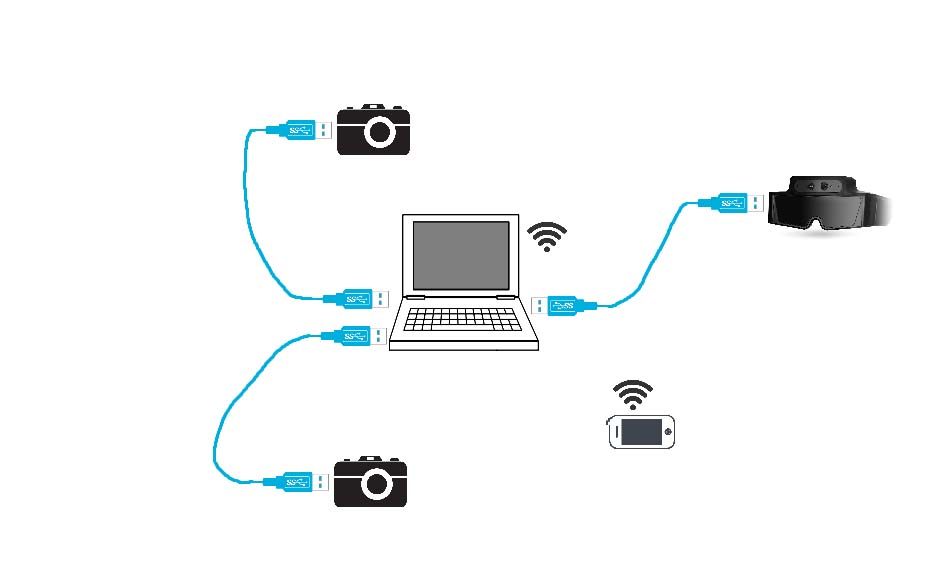
\includegraphics[width=\textwidth]{Entwurf/Hardware_Entwurf.jpg}}{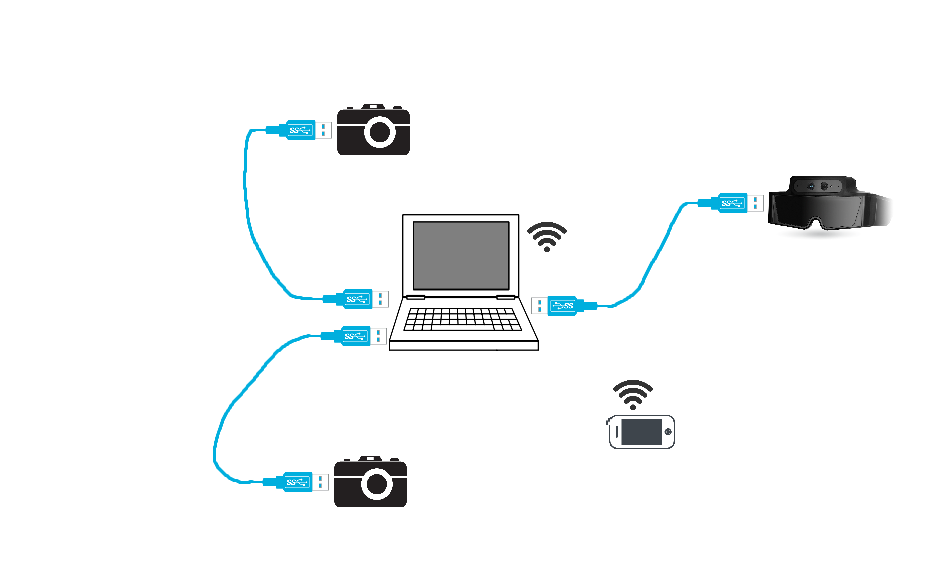
\includegraphics[width=\textwidth]{Entwurf/Hardware_Entwurf.png}}
		\caption{Hardwareaufbau}
		\label{fig:entwurf_hardware}
\end{figure}

\subsection{Komponentendiagramm}
Das Komponentendiagramm bietet eine grobe Übersicht, über die geplanten Interaktionen der Komponenten untereinander.
Eine genauere Beschreibung der einzelnen Komponenten erfolgt im Paketdiagramm.
\begin{figure}[H]
	\centering
	\ifthenelse{\boolean{jpg}}{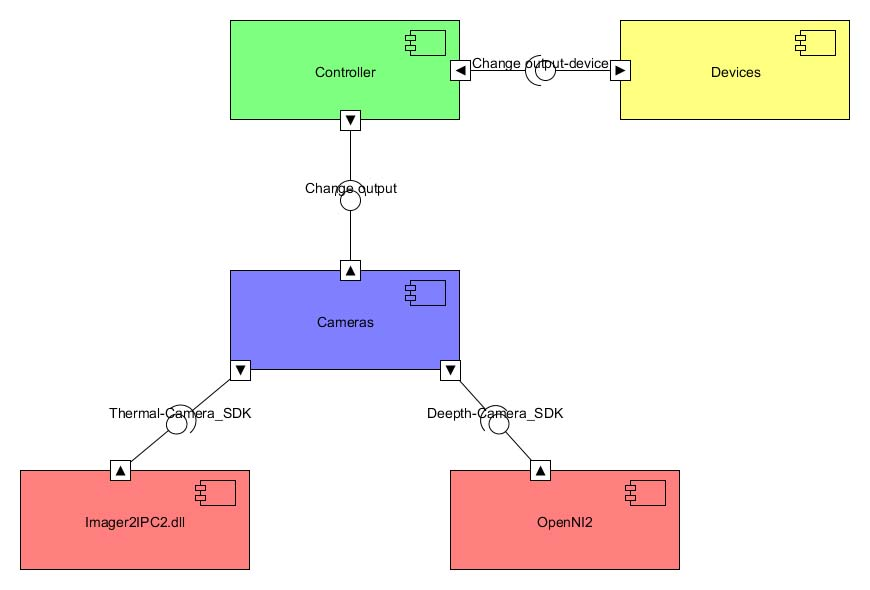
\includegraphics[width=\textwidth]{Entwurf/Komponenten.jpg}}{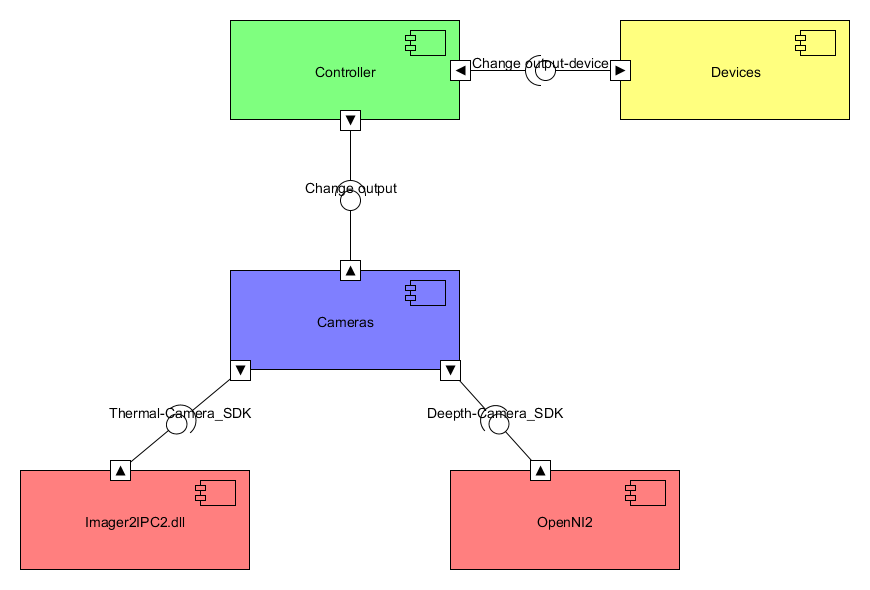
\includegraphics[width=\textwidth]{Entwurf/Komponenten.png}}
	\caption{Komponentendiagramm}
	\label{fig:entwurf_komponenten}
\end{figure}

\section{Beschreibung der einzelnen Komponenten}
Die Komponente Controller ist für den Programmfluss und das Benutzermenü mitsamt Interaktion zuständig.

Die Cameras-Komponente ist der Adapter für die externen Bibliotheken.
Alle bilderstellende und informationsgenerierende Bestandteile sind in dieser Komponente enthalten.

Die Devices-Komponente ist für den Umgang mit allen Ausgabegeräten verantwortlich.
Sämtliche Hardware-Interaktion mit nicht bilderstellenden Geräten wird hier geregelt.

Sowohl die Imager2IPC2 als auch die OpenNI2 Komponente sind externe Bibliotheken, die zur Bilderstellung benötigt werden.

\subsection{Die Komponenten Cameras, Controller und Devices}
\subsubsection{Paketdiagramm}
Das Paketdiagramm verschafft einen Überblick über die in den Komponenten vorkommenden Pakete.
Die einzelnen Pakete werden durch ihre Klassen und deren Methoden spezifiziert.

Während das \textbf{Controller}-Paket Zugriff auf ausgewählte Teile von \textbf{Devices} und \textbf{Camera.net} hat, können diese nicht auf Teile von Controller zugreifen.
Zwischen \textbf{Devices} und \textbf{Camera.net} stehen in keiner Beziehung zueinander.

\textbf{Camera.net} importiert zusätzlich allerdings Funktionen aus den gegebenen Bibliotheken \textbf{Camera SDK}.
Logischerweise ist dies eine einseitige Beziehung.

Damit ist eine hierarchische Ordnung gegebenen.
\begin{figure}[H]
	\centering
	\ifthenelse{\boolean{jpg}}{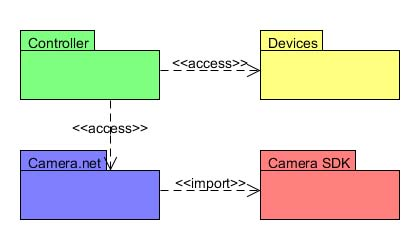
\includegraphics[width=0.6\textwidth]{Entwurf/Paket.jpg}}{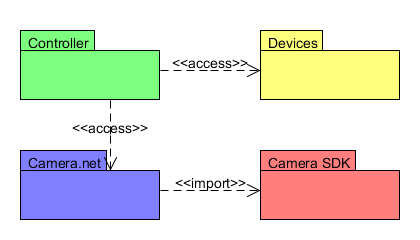
\includegraphics[width=0.6\textwidth]{Entwurf/Paket.png}}
	\caption{Paketdiagramm}
	\label{fig:entwurf_paket}
\end{figure}

\subsubsection{Klassendiagramm}
Das Klassendiagramm dient zur Veranschaulichung der einzelnen Beziehungen zwischen den Paketen und ihren Klassen.
\begin{figure}[H]
	\centering
	\ifthenelse{\boolean{jpg}}{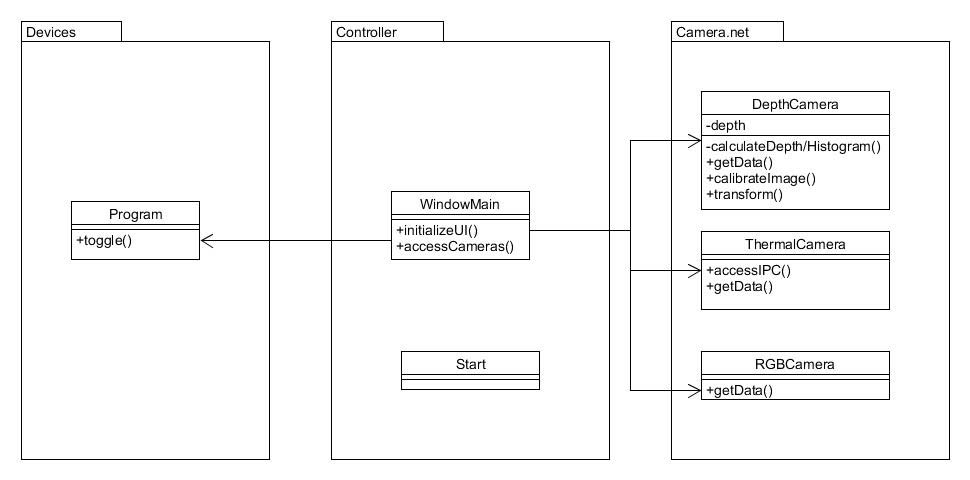
\includegraphics[width=\textwidth]{Entwurf/Klassen.jpg}}{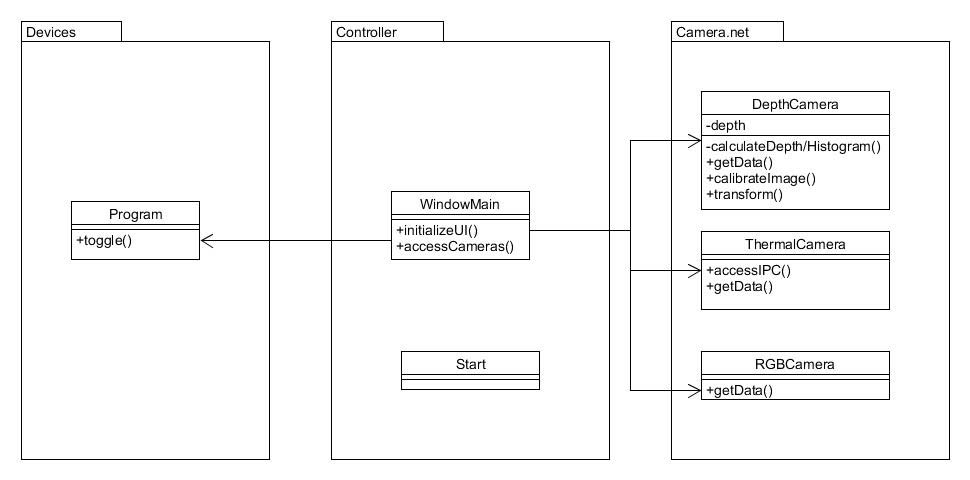
\includegraphics[width=\textwidth]{Entwurf/Klassen.jpg}}
	\caption{Klassendiagramm}
	\label{fig:entwurf_class}
\end{figure}

\subsubsection{Beschreibung}
Die Komponente \textbf{Cameras} besteht aus den Klassen \textit{DepthCamera}, \textit{ThermalCamera}, \textit{RGBCamera}.
Die Klasse \textit{DepthCamera} ist für die Generierung der Tiefenbilder zuständig.
Die Klasse \textit{ThermalCamera} für die Generierung der Wärmebilder verantwortlich.
Zusätzlich wird die Temperatur des Bildmittelpunktes gemessen und der \textit{Viewer}-Klasse zu Verfügung gestellt.
In diesen beiden Klassen können auf die jeweiligen Informationen zugegriffen werden.

Die Klasse \textit{RGBCamera} ist für die Generierung des RGB-Bilds zuständig.

Das Paket \textbf{Controller} besteht aus den Klassen \textit{Form} und \textit{Start}.

Die Klasse \textit{WindowMain} ist zuständig für die Erstellung, Anzeige und Bedienung der Benutzeroberfläche.
Alle auswählbaren Optionen werden von hier aus an die zuständigen Objekte weitergereicht.

Die Klasse \textit{Start} ist zuständig für die Ausführung des Programms und dafür verantwortlich, dass zum Programmstart die gewünschten Windows-Einstellungen gesetzt, sowie zum Programmende die alten wiederhergestellt werden.

Die Klasse \textit{Monitor} ist eine abstrakte Klasse, die die Grundfunktionen jedes Ausgabegerätes enthält.
Dazu gehört das Aktivieren und Deaktivieren eines Ausgabegeräts.

\subsection{Externe Komponenten}
Für die Generierung der Tiefenbilder wird das SDK OpenNI verwendet.
Für die Generierung der Wärmebilder wird die Bibliothek Imager2IPC.dll verwendet.

\section{Versionhistorie}
\begin{description}
	\item [Version 1.0 (27.7.2015)] Erstellung des Dokuments
	\item [Version 1.1 (9.8.2015)] Spezifizierung der Klassen
	\item [Version 1.2 (20.3.2016)] Korrektur des Klassendiagramms
\end{description}
% !TeX spellcheck = de_DE

\chapter{Dilatation}
\label{chap:dilat}

Nach der theoretischen Beschreibung der zu entwickelnden Software, besteht das Problem, dass das Tiefenbild an manchen Stellen flimmert oder auf Grund von Reflexionen teilweise nicht dargestellt werden kann.
Um diesem Problem zu begegnen und ein hochwertigeres Tiefenbild zu erhalten, wurde die Dilatation eingesetzt.

\section{Einleitung}
In der digitalen Bildverarbeitung werden viele Verfahren zur Bildmanipulation verwendet.
Darunter auch die morphologische Bildverarbeitung.
Sie wird unter anderem zur Veränderung der Form von Bildstrukturen eingesetzt.
Im genaueren handelt es sich hierbei also um Operationen auf der Gestalt von Objekten, um diese zu verändern und Störungen zu beseitigen.

\section{Motivation}
Durch das Auftreten von Löchern in der Bildstruktur der Tiefenbildkamera ist es nötig, Bildmanipulationen durchzuführen um die Qualität zu verbessern.
Die Basis hierfür bildet die Erosion und Dilatation, welche die Basisoperationen der Bildverarbeitung darstellen.
Für unser Projekt haben wir die Dilatation verwendet, um die bestmöglichen Ergebnisse zu erzielen.
Hierbei wurde die Dilatation modifiziert, um diese auf ein Tiefenbild anwenden zu können.

\section{Dilatation}
Die Dilatation ermöglicht eine Vergrößerung von Objekten sowie das Schließen von Löchern als auch das Verbinden von Strukturen.
Durch die Verwendung eines Strukturelements wird die Formveränderung erzeugt.
Dieses Strukturelement wird nun schrittweise über das Bild gesetzt.

Hierbei wird, wie in \cref{fig:dilat_dilat} dargestellt, im Tiefenbild ein Tiefenwert gesetzt, wenn letztendlich ein Tiefenwert im Bereich des Strukturelements enthalten ist.
Der gesetzte Tiefenwert ergibt sich aus den Tiefenwerten der Nachbarschaftspixel.
\begin{figure}[H]
	\centering
	\ifthenelse{\boolean{jpg}}{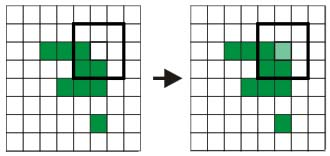
\includegraphics[width=0.5\textwidth]{dilat/dilatation.jpg}}{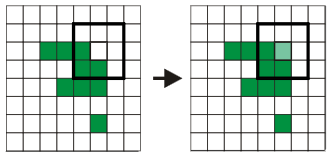
\includegraphics[width=0.5\textwidth]{dilat/dilatation.png}}
	\caption{Dilatationsoperation}
	\label{fig:dilat_dilat}
\end{figure}

\cref{fig:dilat_dilat-change} zeigt die hiermit erreichten Erfolge.

\begin{figure}[H]
	\centering
	\begin{subfigure}[t]{0.45\textwidth}
		\centering
		\ifthenelse{\boolean{jpg}}{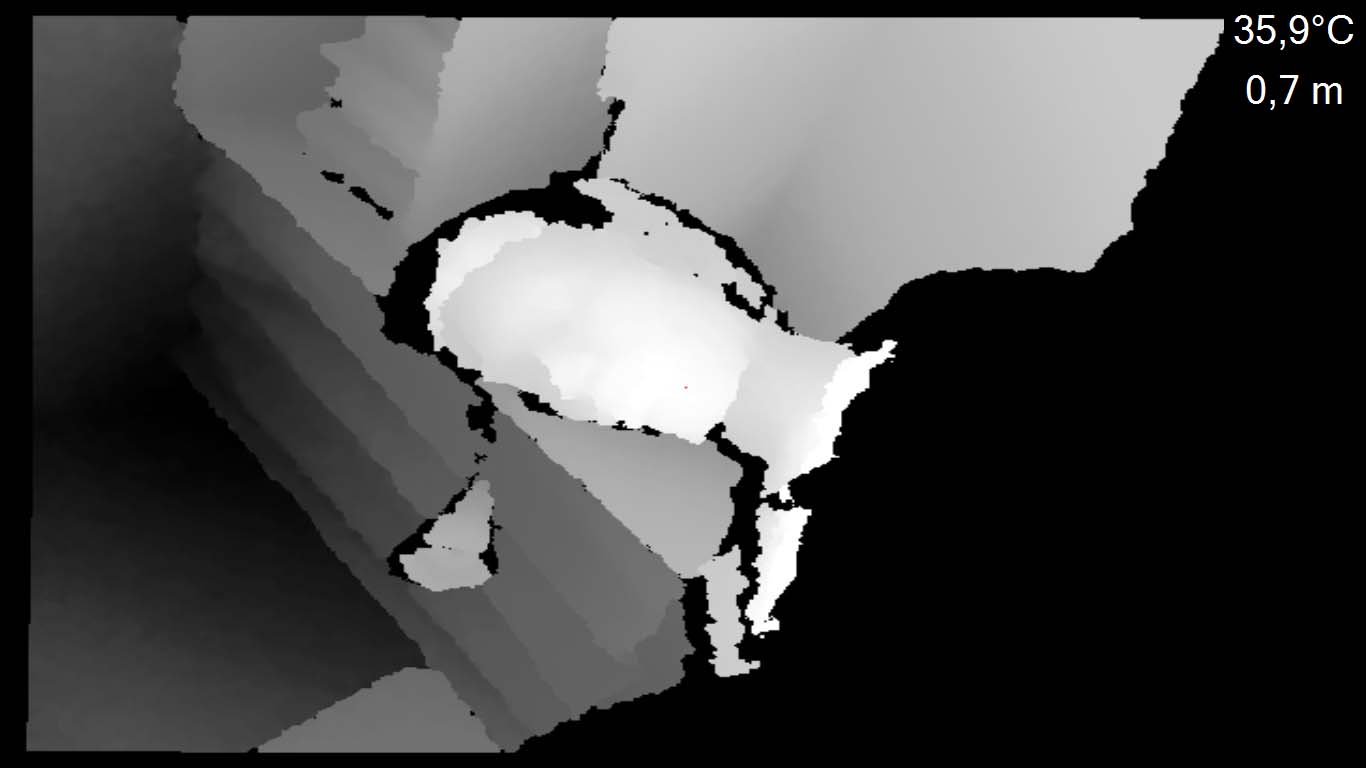
\includegraphics[width=\textwidth]{dilat/ohne-Dilatation.jpg}}{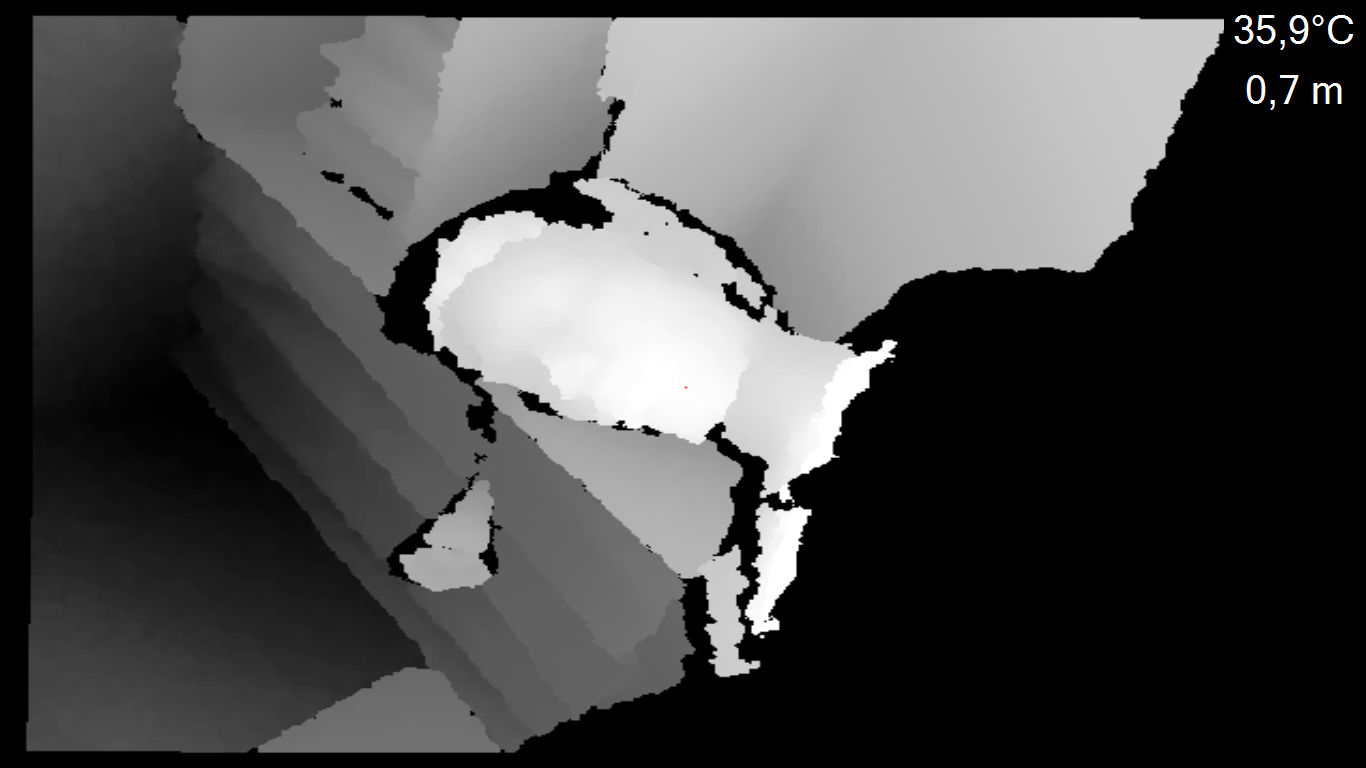
\includegraphics[width=\textwidth]{dilat/ohne-Dilatation.png}}
		\caption{Vor der Dilatation}
		\label{fig:dilat_pre}
	\end{subfigure}
	~
	\begin{subfigure}[t]{0.45\textwidth}
		\centering
		\ifthenelse{\boolean{jpg}}{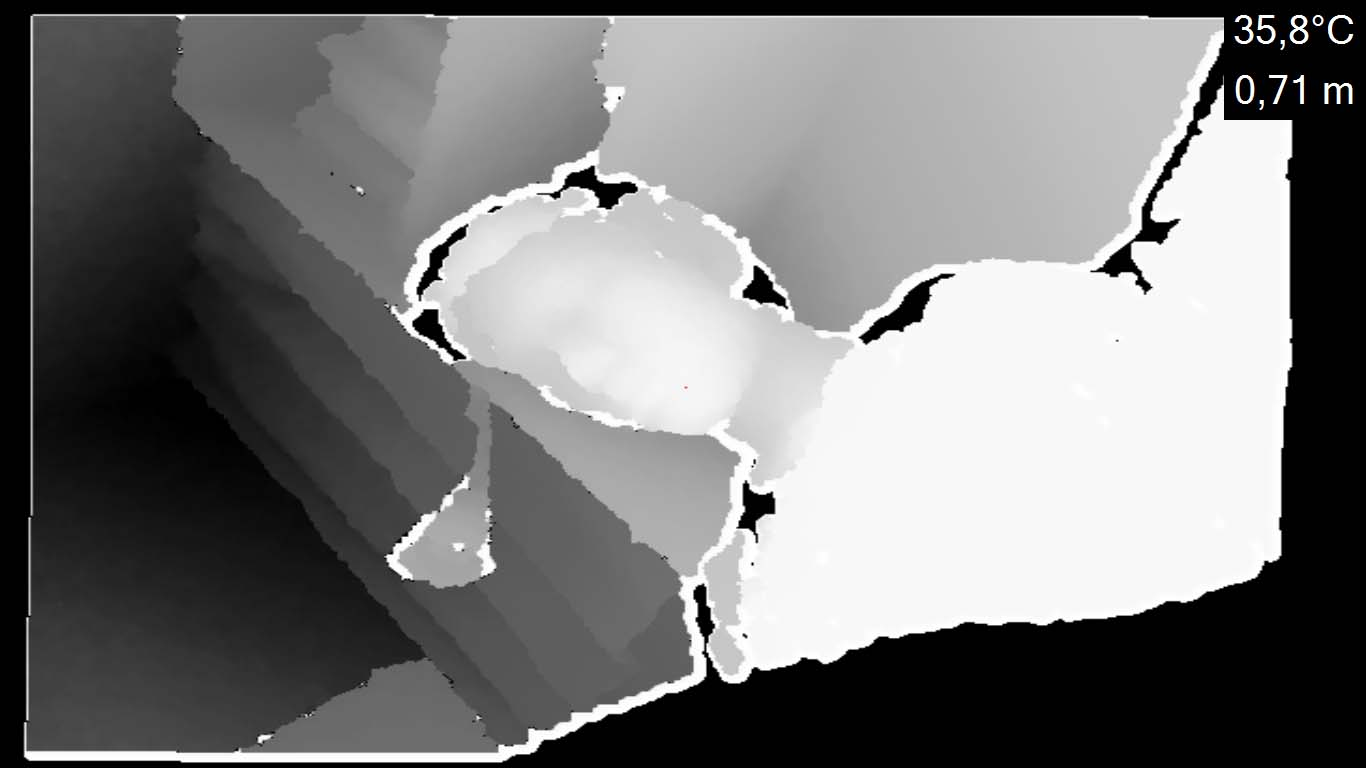
\includegraphics[width=\textwidth]{dilat/mit-Dilatation.jpg}}{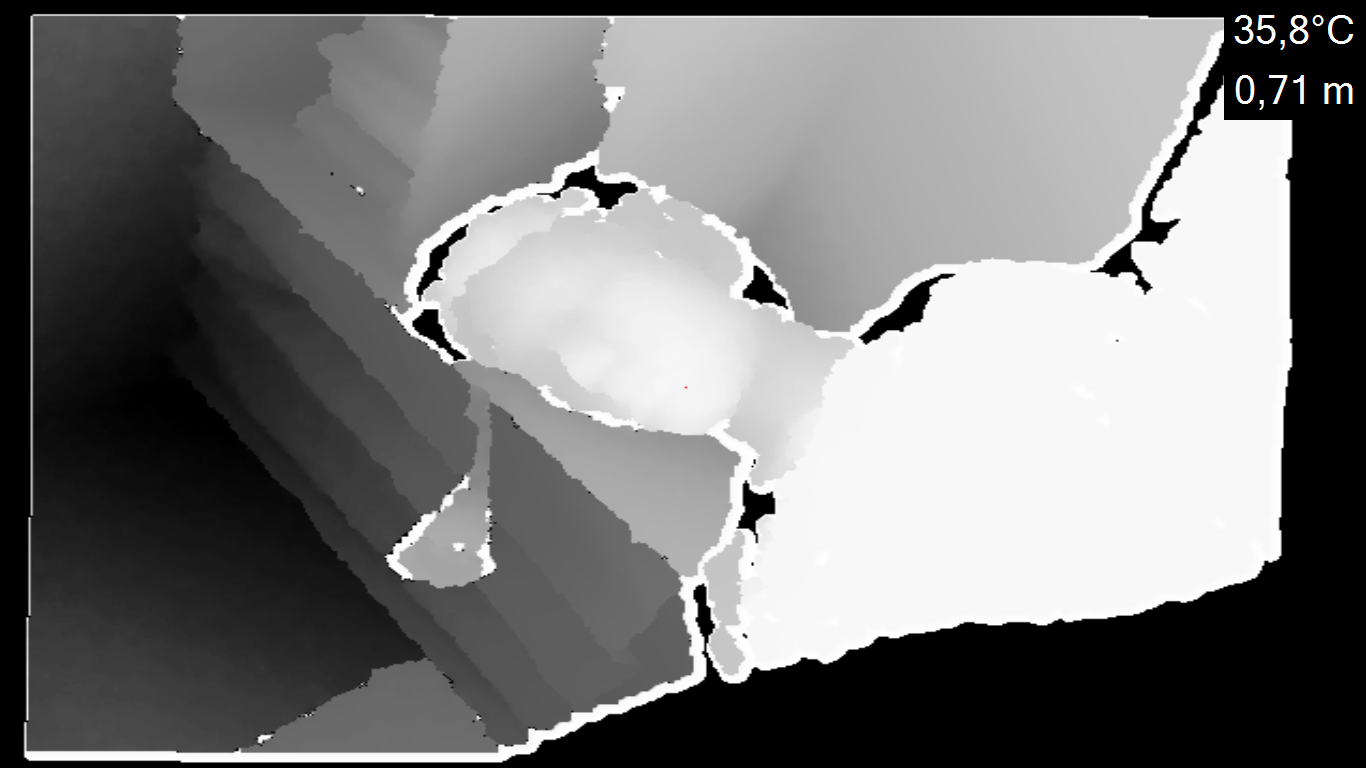
\includegraphics[width=\textwidth]{dilat/mit-Dilatation.png}}
		\caption{Nach der Dilatation}
		\label{fig:dilat_post}
	\end{subfigure}
	\caption{Effekte der Dilatation}
	\label{fig:dilat_dilat-change}
\end{figure}
% !TeX spellcheck = de_DE

\chapter{Kalibrierung}
\label{chap:calibration}

Nachdem im vorherigen Kapitel auf die Methode der Dilatation zur Verbesserung des erstellten Tiefenbildes eingegangen wurde, wird in diesem Kapitel der Vorgang der Kalibrierung beschrieben.

\section{Ziele der Kalibrierung}
Das Ziel bei unserer Kalibrierung ist es die Bilder zweier verschiedener Kameras aufeinander anzupassen, sodass in beiden Kameras das gleiche Bild angezeigt wird.

\begin{figure}[h]
	\centering
	\begin{subfigure}[t]{0.45\textwidth}
		\centering
		\ifthenelse{\boolean{jpg}}{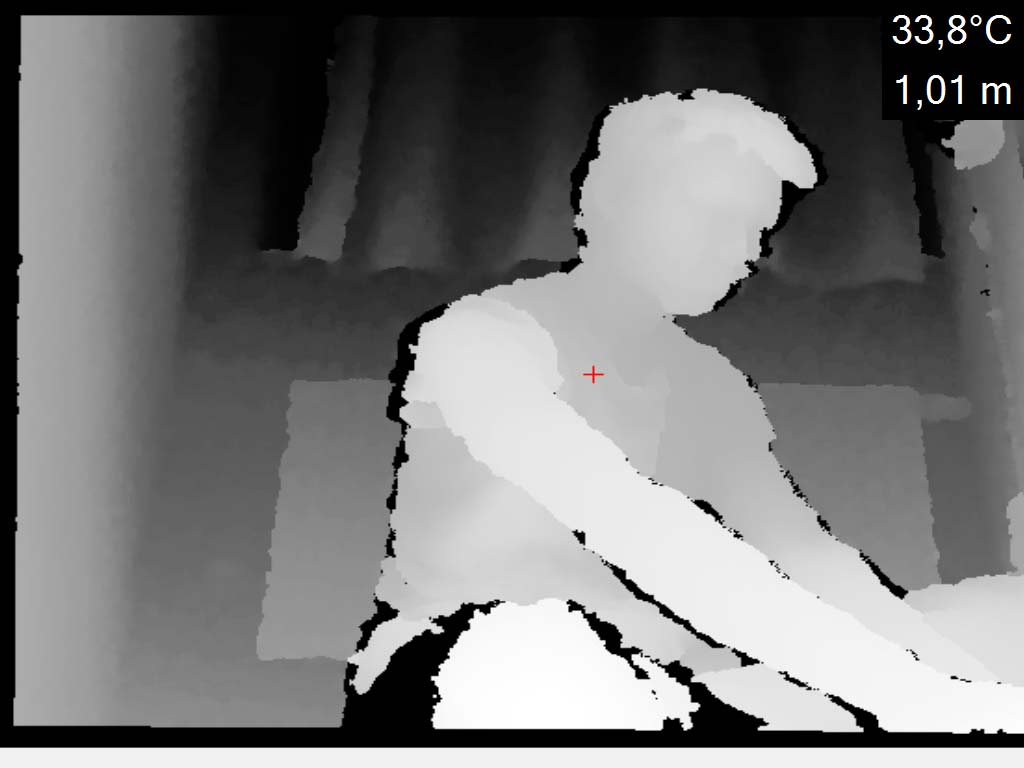
\includegraphics[width=\textwidth]{Kalibrierung/pre_depth.jpg}}{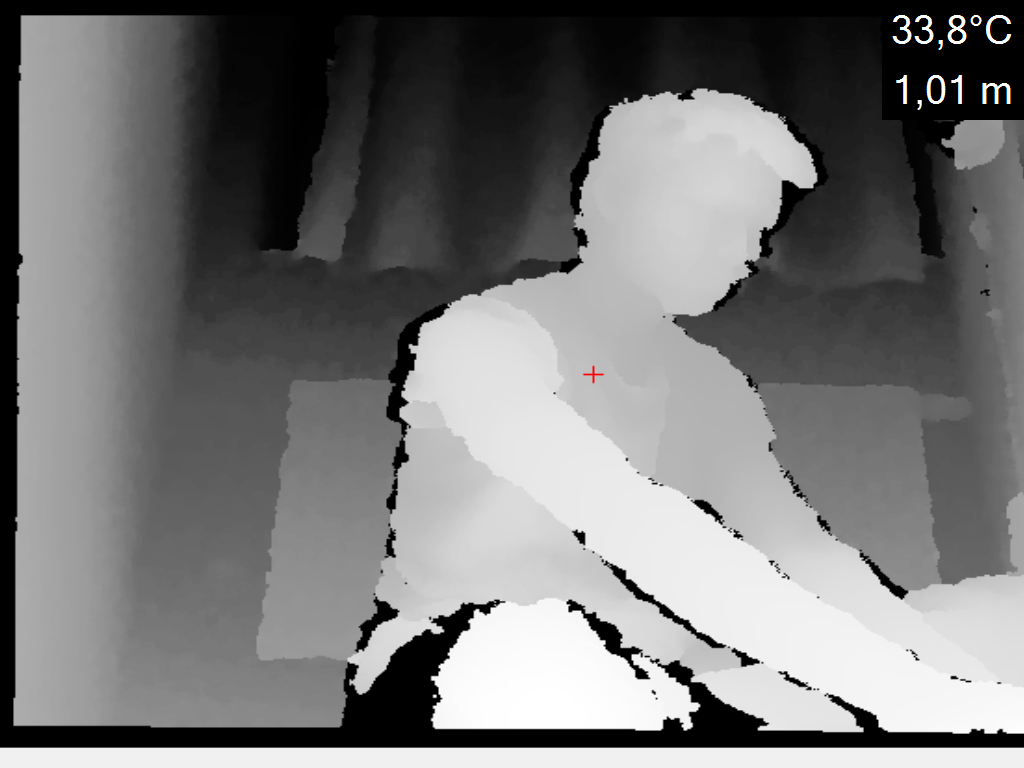
\includegraphics[width=\textwidth]{Kalibrierung/pre_depth.png}}
		\caption{Tiefenbild}
		\label{fig:calib_pre_deepth}
	\end{subfigure}
	~
	\begin{subfigure}[t]{0.45\textwidth}
		\centering
		\ifthenelse{\boolean{jpg}}{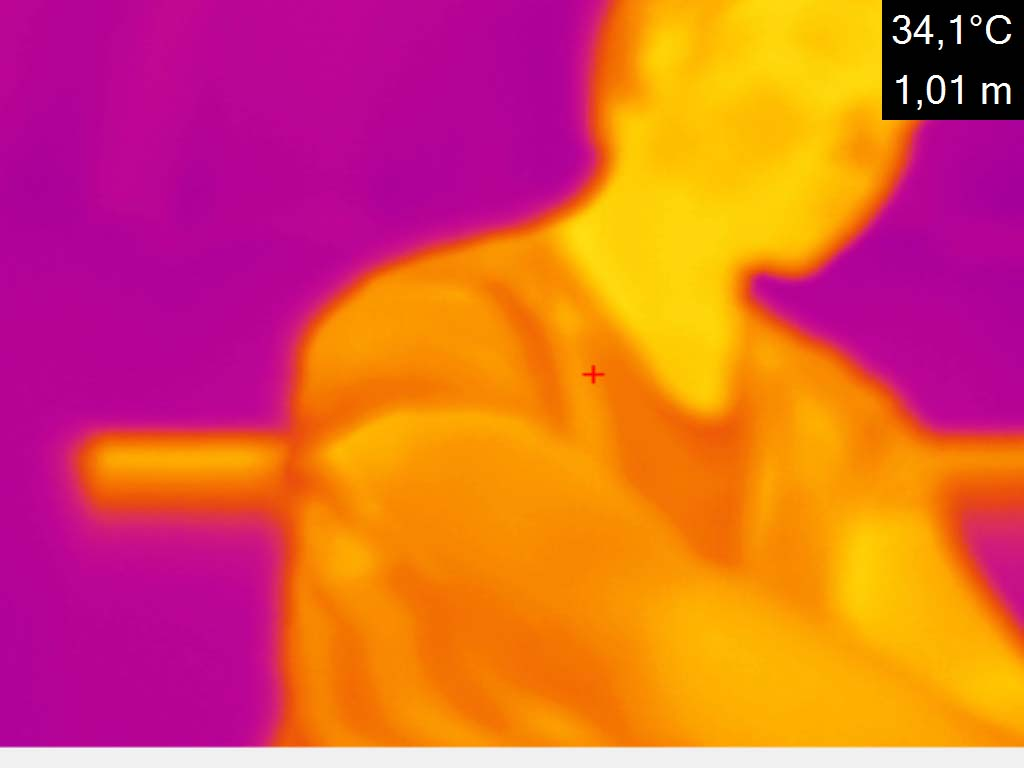
\includegraphics[width=\textwidth]{Kalibrierung/pre_heat.jpg}}{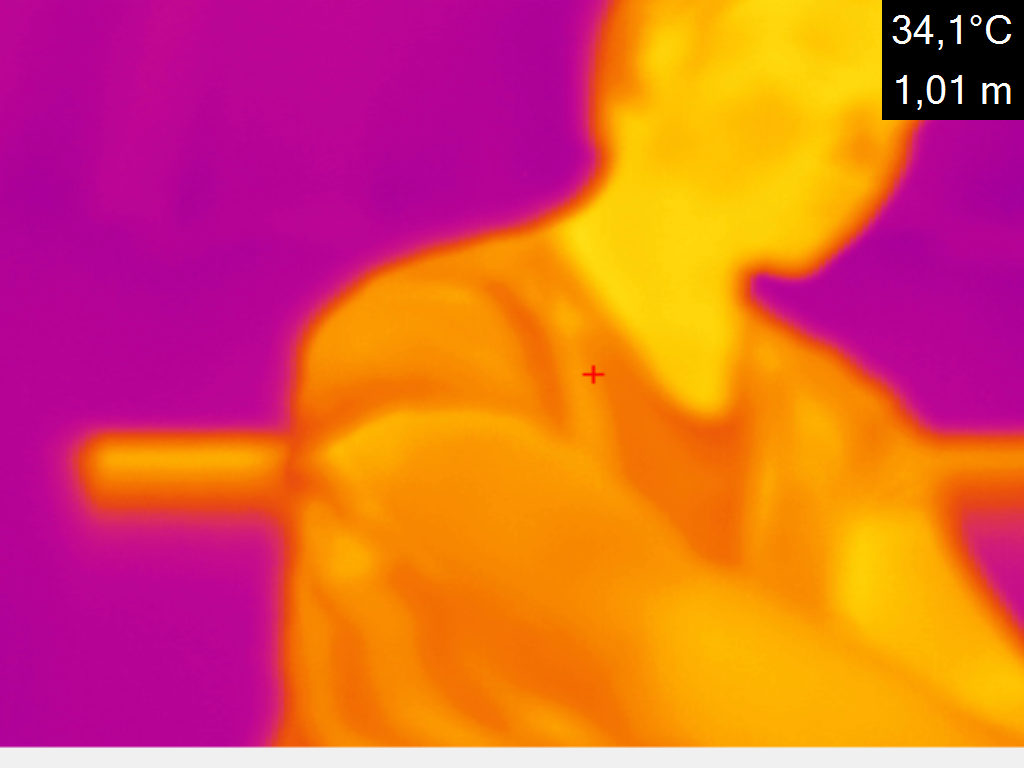
\includegraphics[width=\textwidth]{Kalibrierung/pre_heat.png}}
		\caption{Wärmebild}
		\label{fig:calib_pre_heat}
	\end{subfigure}
	\caption{Kamerabilder vor der Kalibrierung}
	\label{fig:calib_pre}
\end{figure}

\begin{figure}[h]
	\centering
	\begin{subfigure}[t]{0.45\textwidth}
		\centering
		\ifthenelse{\boolean{jpg}}{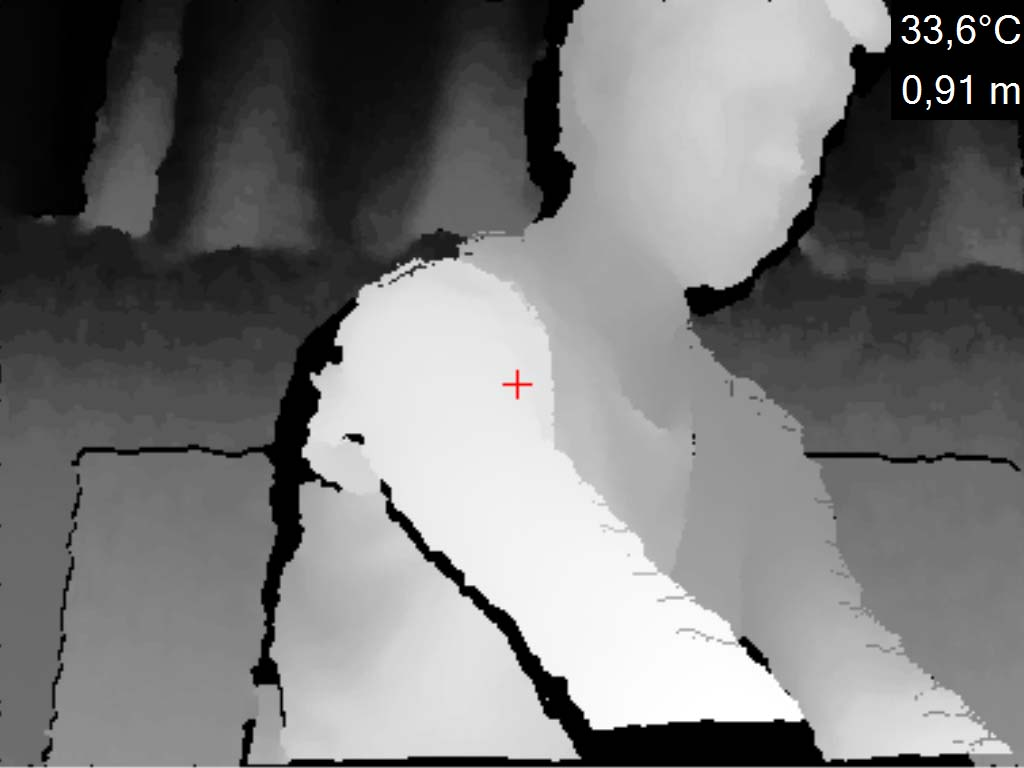
\includegraphics[width=\textwidth]{Kalibrierung/post_depth.jpg}}{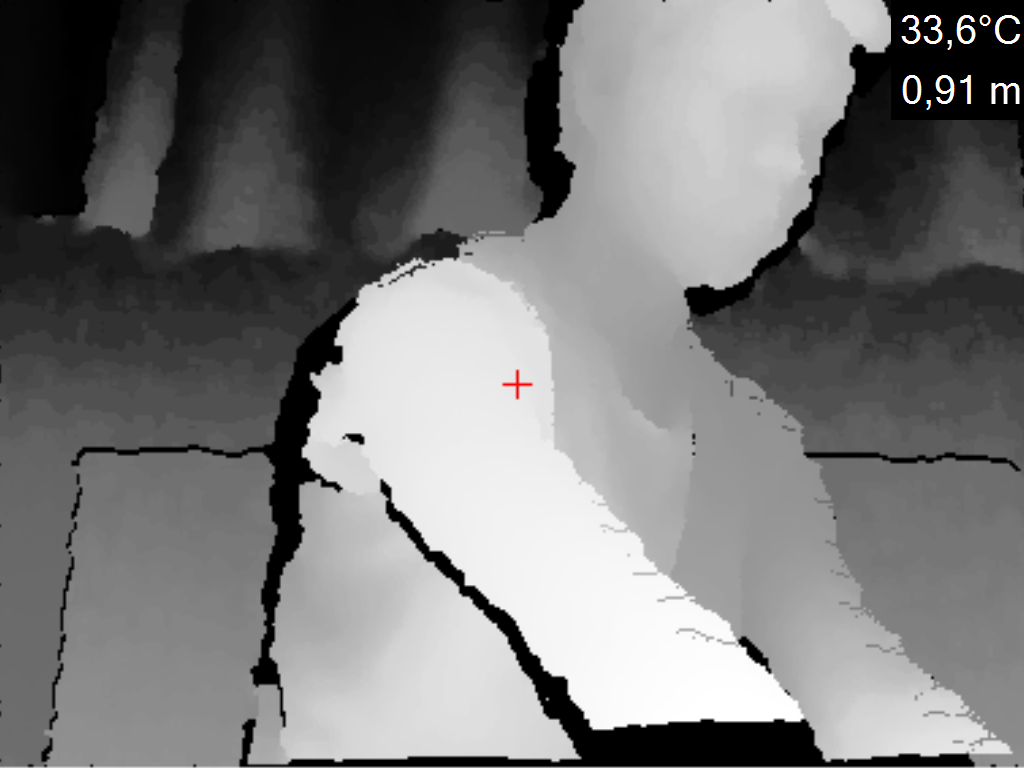
\includegraphics[width=\textwidth]{Kalibrierung/post_depth.png}}
		\caption{Tiefenbild}
		\label{fig:calib_post_deepth}
	\end{subfigure}
	~
	\begin{subfigure}[t]{0.45\textwidth}
		\centering
		\ifthenelse{\boolean{jpg}}{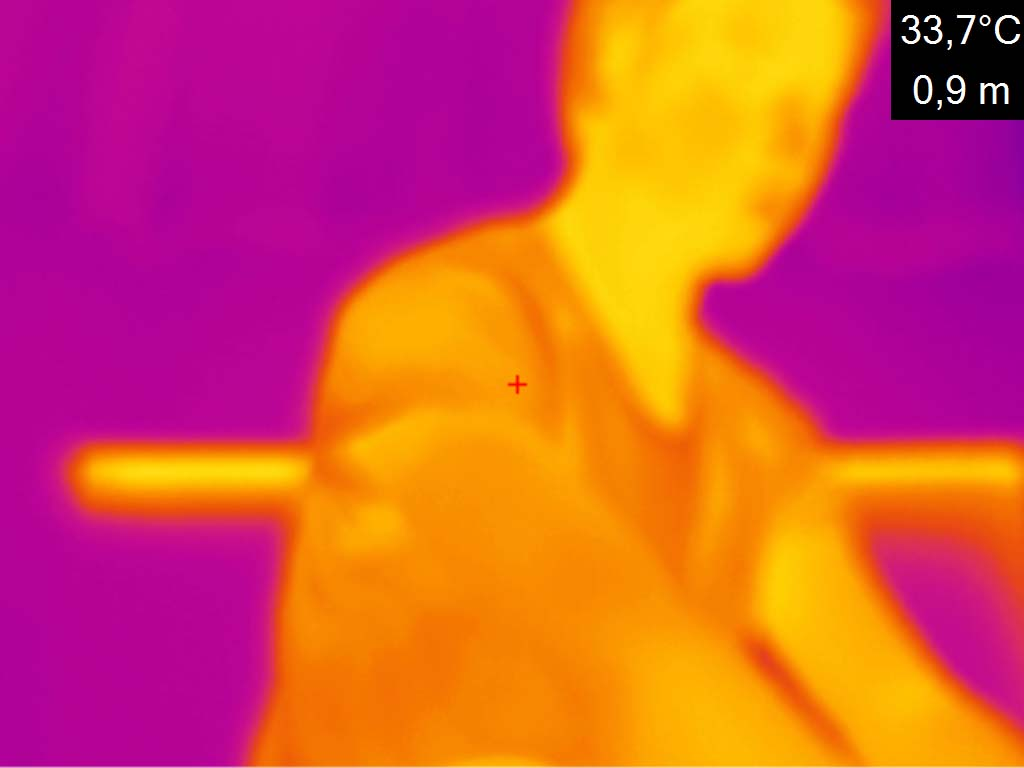
\includegraphics[width=\textwidth]{Kalibrierung/post_heat.jpg}}{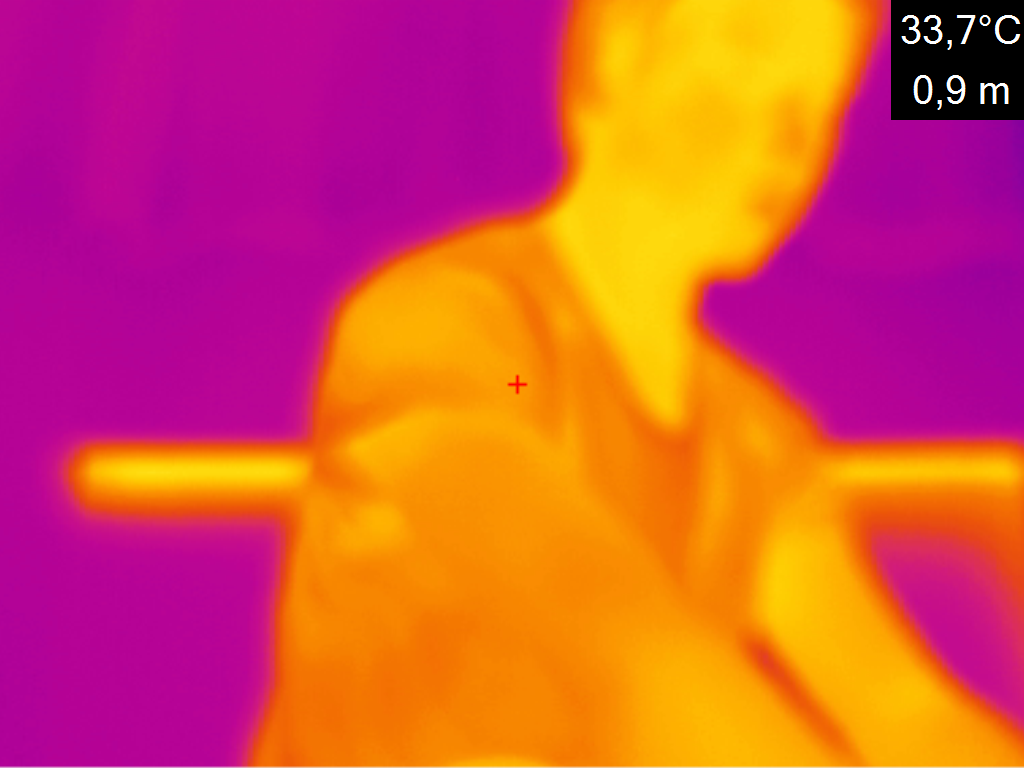
\includegraphics[width=\textwidth]{Kalibrierung/post_heat.png}}
		\caption{Wärmebild}
		\label{fig:calib_post_heat}
	\end{subfigure}
	\caption{Kamerabilder nach der Kalibrierung}
	\label{fig:calib_ost}
\end{figure}

Dafür werden benötigt:
\begin{description}
	\item[intrinsischer Kameraparameter] Bestehend aus:
	\begin{itemize}
		\item Fokallänge (focal length) 
		\item Bildmittelpunkt (principal point)
	\end{itemize}
	\item[extrinsischer Kameraparameter] Bestehend aus:
	\begin{itemize}
		\item Rotationsmatrix
		\item Translationsmatrix
	\end{itemize}
\end{description}

\section{Berechnung der intrinsischen und extrinsischen Kameraparameter}
Diese intrinsischen und extrinsischen Kameraparameter wurden für uns in MATLAB mithilfe der Computer Vision Toolbox berechnet.
\begin{figure}[h]
	\centering
	\ifthenelse{\boolean{jpg}}{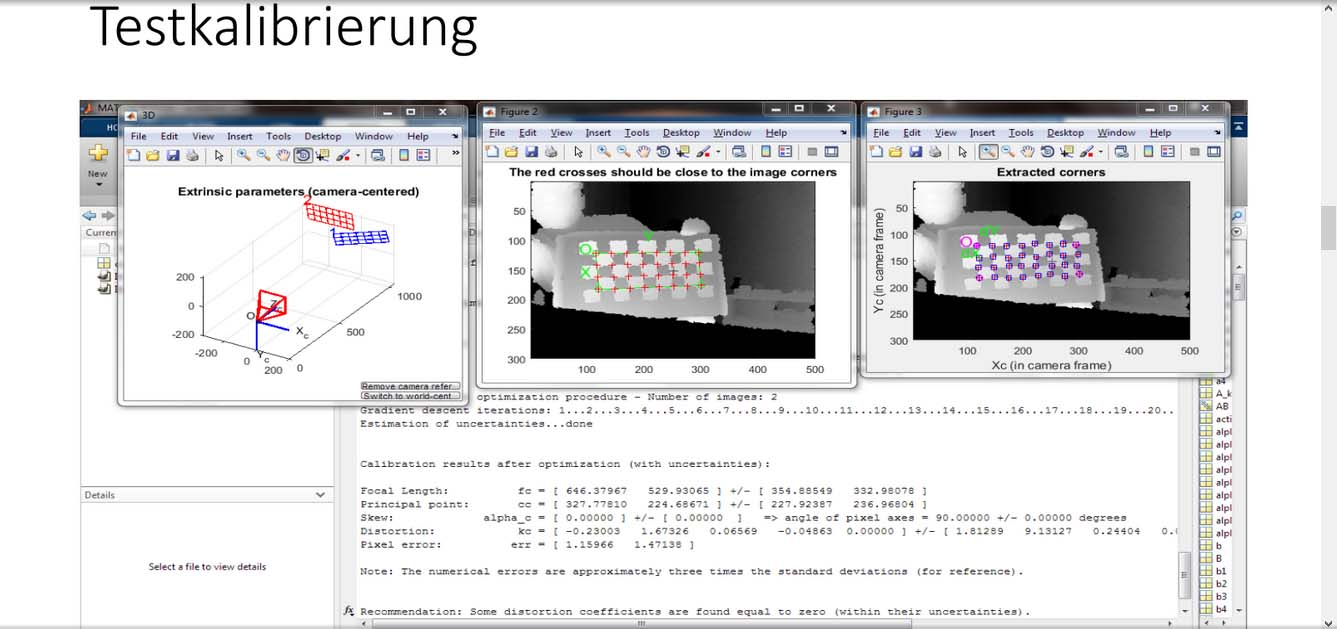
\includegraphics[width=\textwidth]{Kalibrierung/MatLab.jpg}}{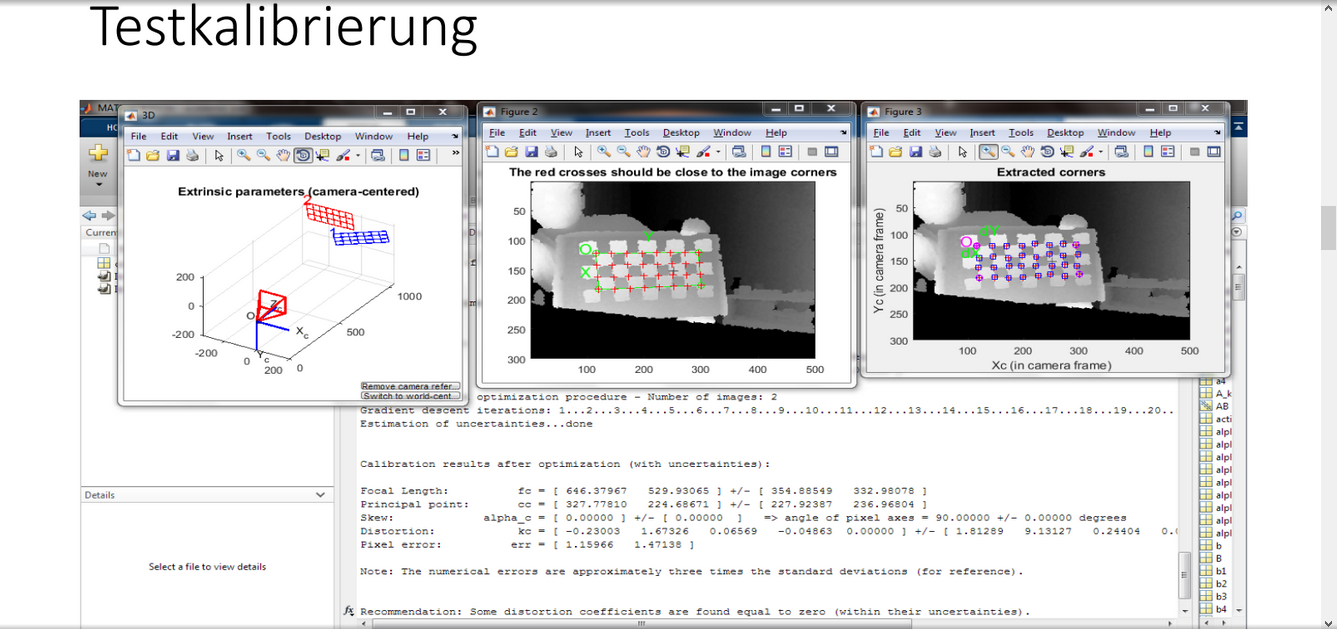
\includegraphics[width=\textwidth]{Kalibrierung/MatLab.png}}
	\caption{Testkalibrierung mit MATLAB}
	\label{fig:calib_matlab}
\end{figure}

\subsection{Vorgehen}
Es werden von den beiden zu kalibrierenden Sensoren Bilder von einem Schachbrett gemacht.
Dabei sollten diese Bilder möglichst aus verschiedene Positionen und und Winkeln erstellt werden.
Mithilfe von MATLAB kann dann durch diese Bilder die intrischen Kameraparameter und extrinsischen Kameraparameter, welche die Position zwischen den beiden Sensoren beschreibt berechnet werden.
\begin{figure}[h]
	\centering
	\ifthenelse{\boolean{jpg}}{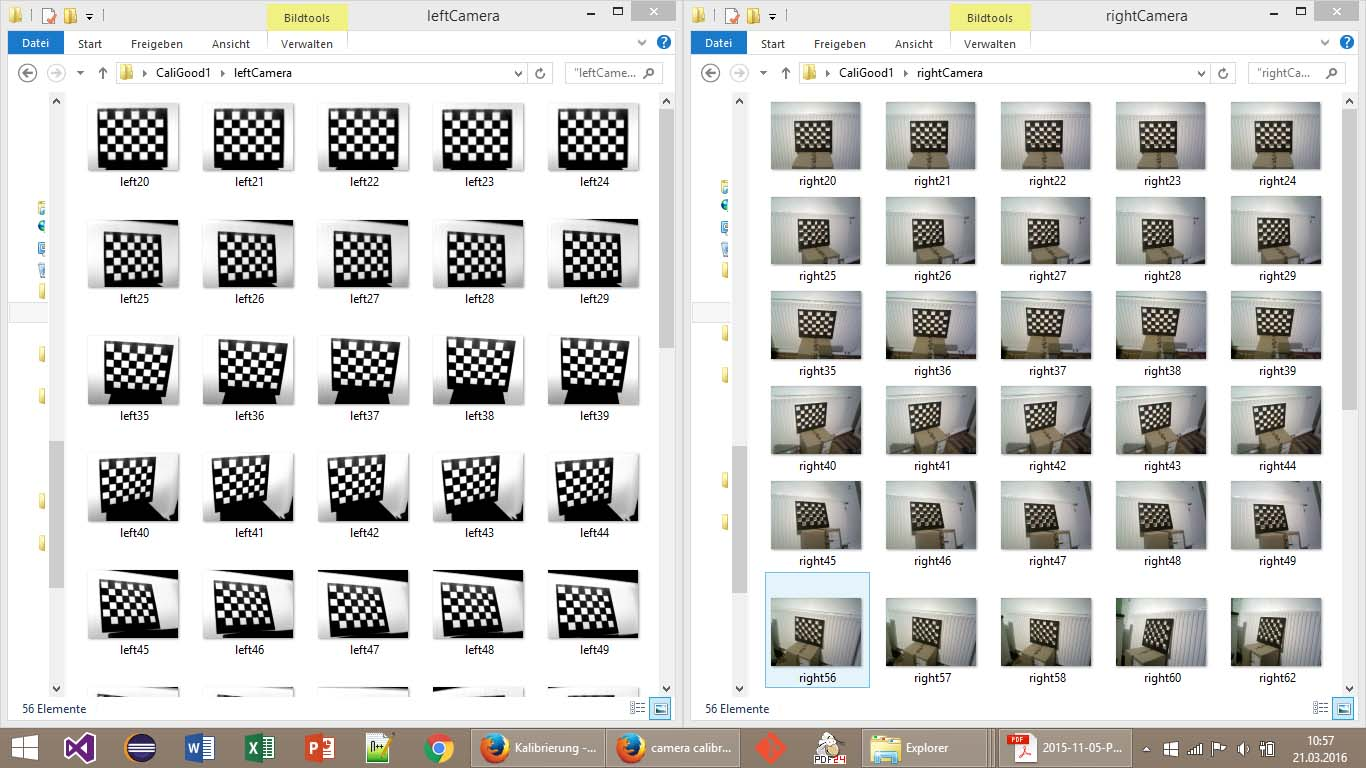
\includegraphics[width=\textwidth]{Kalibrierung/pics.jpg}}{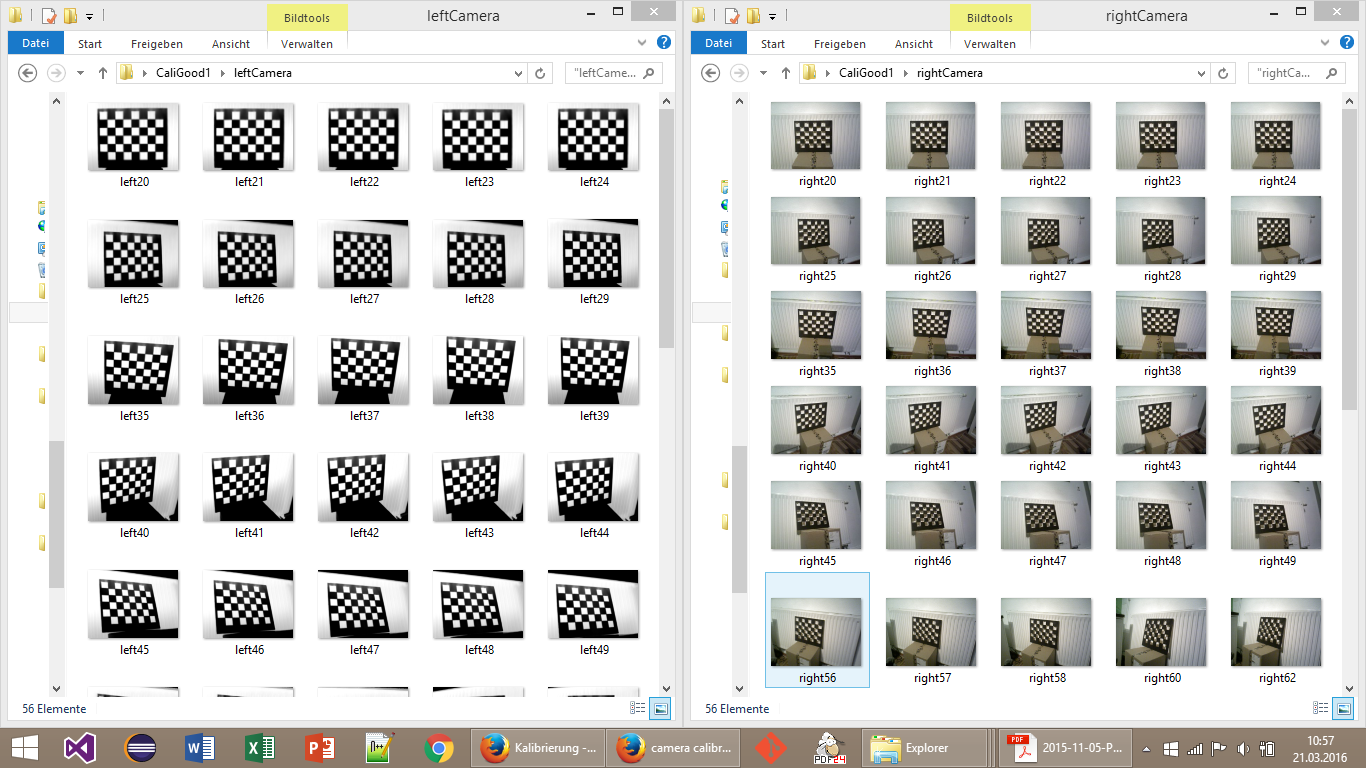
\includegraphics[width=\textwidth]{Kalibrierung/pics.png}}
	\caption{Auszug der für die Kalibrierung erstellten Bilder}
	\label{fig:calib_pics}
\end{figure}
Mithilfe der oben genannten Werten konnten wir jedes Pixel im Tiefenbild seinem zugehörigen Pixel im Wärmebild zuweisen.

\section{Kalibrierung Tiefenbild auf Wärmebild Technischer Vorgang}

\subsection{Vorgang}
\begin{enumerate}
	\item \textbf{Umwandlung Bildkoordinaten (\bzgl Tiefenbildsensor) zu Weltkoordinaten(\bzgl Tiefensensor)}
	
	Dazu wurde jedes Pixel mit den Bildkoordinaten unseres Bitmapbildes (\textbf{x},\textbf{y}) und seiner zugehörigen Distanz \textbf{z} (durch den Tiefensensor ermittelt) mithilfe der intrinsischen Kameraparameter des Tiefensensors in Weltkoordinaten(\bzgl Tiefensensor) umgewandelt.
	
	\item \textbf{Umwandlung Weltkoodinaten (\bzgl Tiefensensor) zu Weltkoordinaten (\bzgl Wärmesensor)}
	
	Diese Weltkoordinaten (\bzgl Tiefensensor) wurde dann mithilfe der extrinsischen Kameraparameter (Rotation und Translation) in die Weltkoordinaten (\bzgl Wärmesensors) umgewandelt.
	
	\item \textbf{Umwandlung Weltkoordinaten (\bzgl Wärmesensor) zu Bildkoordinaten(\bzgl Tiefenbildsensor)}
	
	Diese Weltkoordinaten (\bzgl Wärmesensor) werden dann mithilfe der intrinsischen Kameraparameter des Wärmesensors in die Bildkoordinaten (\bzgl Tiefenbildsensor) umgewandelt.
	
	Durch diese 3 Schritte können wir herausfinden, wo ein eingezeichnetes Pixel des Tiefenbildsensor sich im Bild des Wärmesensors befinden würde.
	Dadurch können wir diese Pixel dann an ihren neuen Ort verschieben.
\end{enumerate}

\subsection{Technische Details}
In unserem Projekt konnten wir die Objekte welche zwischen 1.7m und 3.7m vom Tiefenbildsensor entfernt sind genau zwischen Tiefenbildsensor und Wärmesensor kalibrieren.
Objekte zwischen 0.6m und 1.7m oder 3.7m und 8m werden, nachträglich mithilfe einer Funktion welche abhängig von der Entfernung ist, manuell nach verschoben.

Außerdem wurde bei uns bei der Berechnung der intrinsischen und extrinsischen Kameraparameter nicht Bilder des Tiefenbildsensors verwendet sondern einer RGB-Kamera welche bereits zuvor vom Hersteller aufeinander kalibriert wurde.
Grund für dies war die schlechte Erkennung des Schachbretts durch den Tiefenbildsensor.
% !TeX spellcheck = de_DE

\chapter{Bildmodifusion}
\label{chap:fusion}

Nachdem im vorherigen Kapitel auf die Methode der Dilatation zur Verbesserung des erstellten Tiefenbildes eingegangen wurde, wird in diesem Kapitel der Vorgang der Kalibrierung beschrieben.
Dabei werden zuerst Problematiken der einzelnen Kameras beschrieben, um ein Verständnis für die auszugleichenden Schwächen zu schaffen.
Danach werden die betrachteten Fusionsmöglichkeiten und der Grund für ihr Verwerfen genannt, sowie die letztendlich gewählte Fusionsart beschrieben.

\section{Vor- und Nachteile der Kameras}
Um eine qualitative Fusion zu erreichen, muss ein Verständnis für die Stärken und Schwächen der jeweilig verwendeten Systeme vorhanden sein.
Im folgenden werden die für relevant erachteten Einschränkungen aufgelistet.

\subsection{Wärmebildkamera}
%\subsubsection{Wärmebildkamera}
\begin{center}
	\begin{tabular}{| p{7.5cm} | p{7.5cm} |}
		\hline
		Vorteile & Nachteile \\ \hline
		
		\begin{itemize}
			\item Kann Temperaturunterschiede darstellen
			\item Zeichnet sehr gute Konturen bei geringen Temperaturunterschieden
			\item Große Reichweite
			\item Ermöglicht Sicht durch diverse Materialien
		\end{itemize} & \begin{itemize}
			\item Wärmereflexion an vielen Materialien
			\item Schlechte Bildqualität bei nahezu nicht vorhandenem Temperaturunterschied
			\item \enquote{Wärmeflecken} an Orten, wo zuvor ein warmes Objekt war
			\item Geringere Auflösung / Kleinerer Blickwinkel
		\end{itemize} \\ 
		\hline
	\end{tabular}
\end{center}

\subsection{Tiefenbildkamera}
%\subsubsection{Tiefenbildkamera}
\begin{center}
	\begin{tabular}{| p{7.5cm} | p{7.5cm} |}
		\hline
		Vorteile & Nachteile \\ \hline
		
		\begin{itemize}
			\item Gute Darstellung von Konturen größerer Objekte
			\item Größere Auflösung / Größerer Blickwinkel
		\end{itemize} & \begin{itemize}
			\item Eingeschränkte Reichweite (\ca 0,5m - 7,5m)
			\item Flimmerndes Bild
			\item Teilweise werden kurze Distanzen nicht gut dargestellt
			\item Einige Materialien reflektieren
			\item Reflexion bei gewissem Haltungswinkel
			\item Einzelne Objektdetails schwerer zu erkennen
		\end{itemize} \\ 
		\hline
	\end{tabular}
\end{center}

\section{Explorierte Fusionsmöglichkeiten}
In diesem Abschnitt werden die genauer betrachteten Fusionsmöglichkeiten und der Grund für ihr verwerfen diskutiert.
Dabei sind in einigen der Abbildungen nicht die optimierten Bildarten integriert, da diese Möglichkeiten bereits früher verworfen wurden.

\subsection{Parallele Anzeige beider Modi}
Das Tiefenbild und das Wärmebild werden wie in \cref{fig:fusion_both} entweder nebeneinander oder übereinander angezeigt.
Dadurch könnten beide Bildmodi verlustfrei angezeigt werden, allerdings würden die Probleme nur begrenzt verringert werden.
\begin{figure}[H]
	\centering
	\begin{subfigure}[t]{0.25\textwidth}
		\centering
		\ifthenelse{\boolean{jpg}}{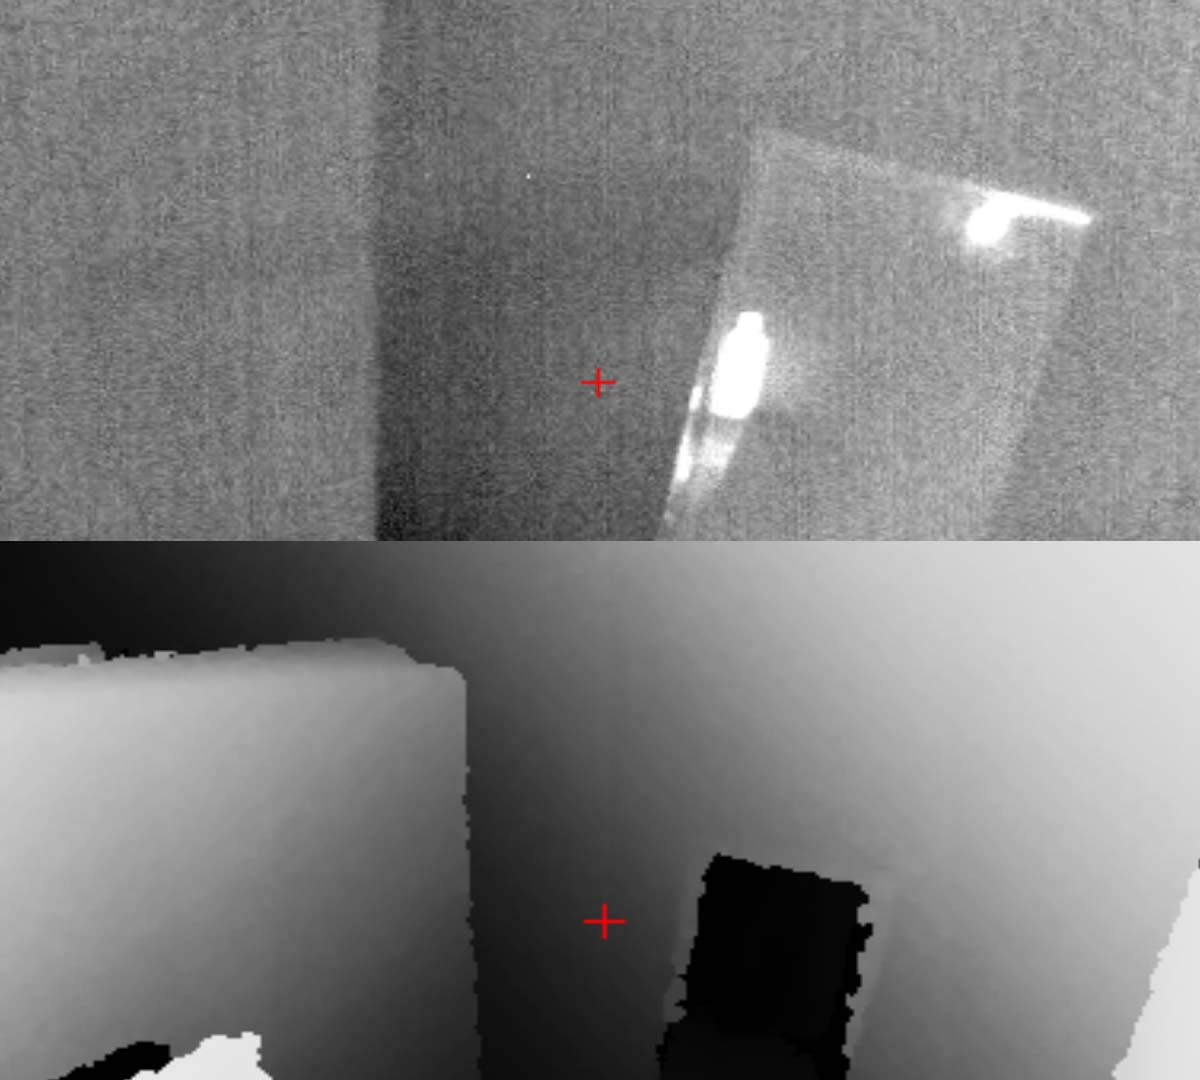
\includegraphics[width=\textwidth]{Fusion/over.jpg}}{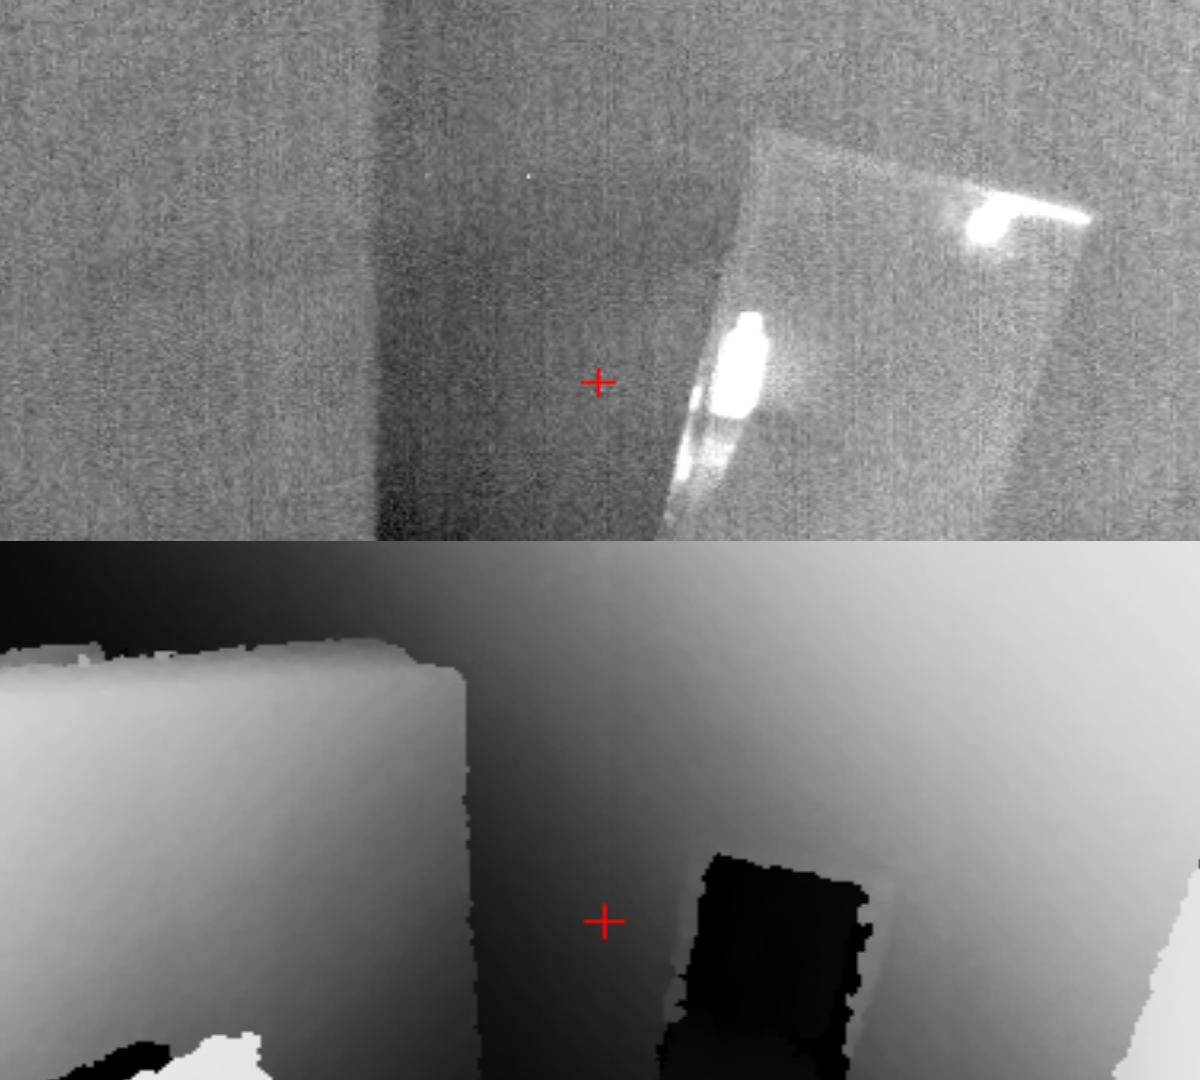
\includegraphics[width=\textwidth]{Fusion/over.png}}
		\caption{Anzeige beider Modi übereinander}
		\label{fig:fusion_both_over}
	\end{subfigure}
	~
	\begin{subfigure}[t]{0.65\textwidth}
		\centering
		\ifthenelse{\boolean{jpg}}{
\includegraphics[width=\textwidth]{Fusion/besides.jpg}}{
\includegraphics[width=\textwidth]{Fusion/besides.png}}
		\caption{Anzeige beider Modi nebeneinander}
		\label{fig:fusion_both_besides}
	\end{subfigure}
	\caption{Parallele Anzeige von beiden Kameramodi}
	\label{fig:fusion_both}
\end{figure}

Dieser Ansatz wurde verworfen, da dieser Ansatz keine wirkliche Fusion darstellt und bei internen Tests einige Teilnehmer noch Schwierigkeiten hatten, Objekte auf beiden Teilen zu lokalisieren.
Auch wirkte sich dieser Ansatz negativ auf das mobile Anzeigegerät, da die Anzeige bereits aus kurzer Entfernung für zu klein befunden wurde.

\subsection{Ersetzen des Tiefenbild mit Wärmebild}
\label{sec:fusion_overwrite}
\cref{fig:fusion_overwrite} zeigt, dass das Wärmebild über den Bildteil des normalen Tiefenbildes gelegt wird.
Problematisch hierbei ist, dass lediglich der Vorteil des größeren Bildausschnitts der Tiefenbildkamera genutzt wird.
Alle anderen Probleme bestehen weiterhin.
Zudem wurde, in Abstimmung mit den Projektbetreuern, entschieden, dass der unterschiedlich große Bildausschnitt, beider Kameras nicht beachtet und durch verkleinern der Auflösung der Tiefenbildkamera eliminiert wird, da dies durch ein anderes Objektiv der Wärmebild gelöst werden könnte.
\begin{figure}[H]
	\centering
	\ifthenelse{\boolean{jpg}}{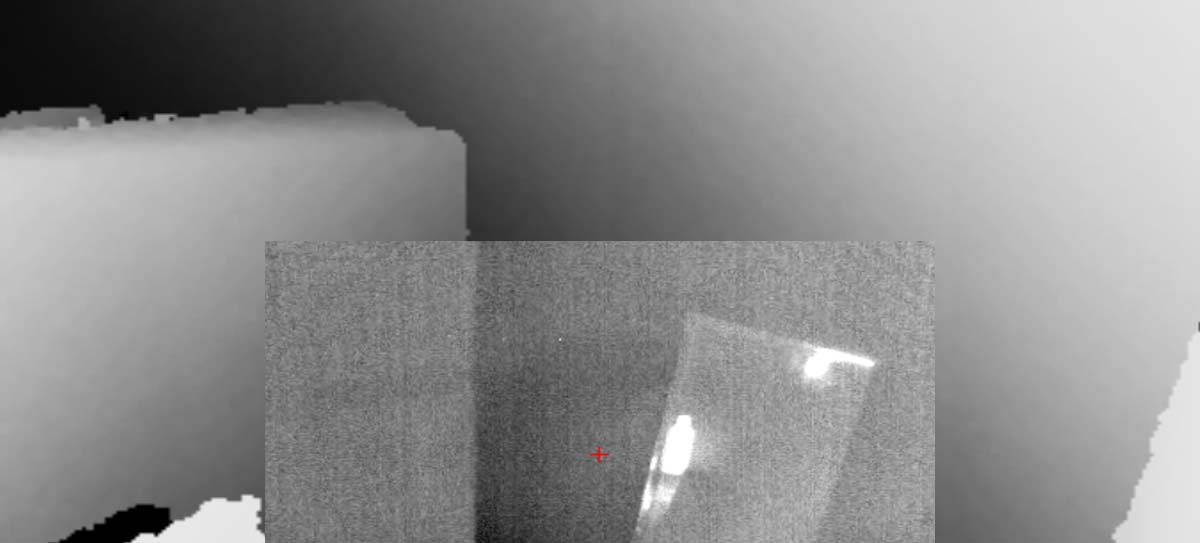
\includegraphics[width=0.9\textwidth]{Fusion/overwrite.jpg}}{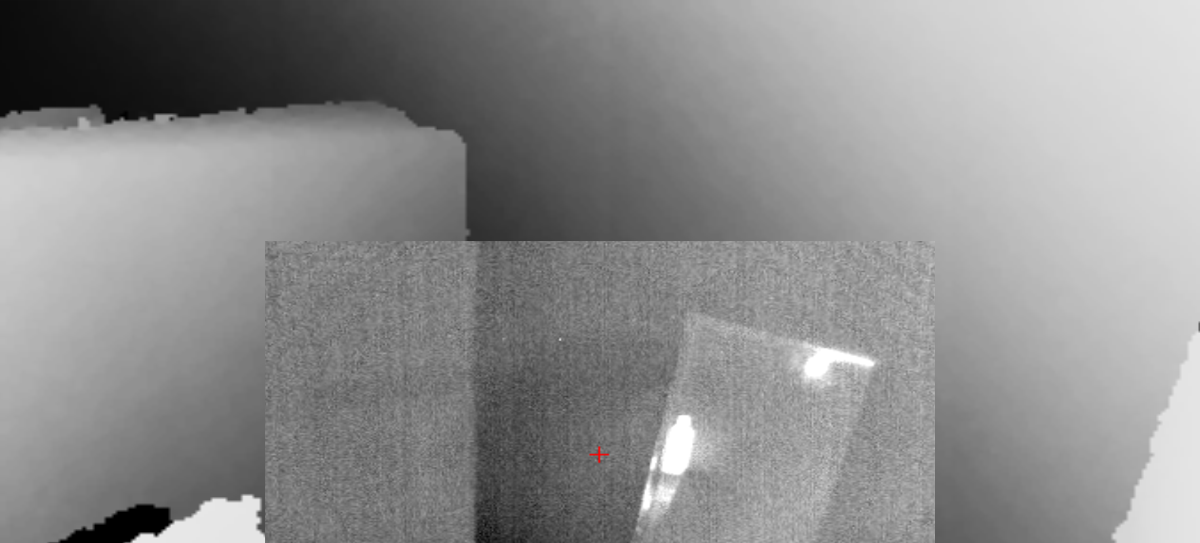
\includegraphics[width=0.9\textwidth]{Fusion/overwrite.png}}
	\caption{Ersetzung eines Teiles des Tiefenbildes mit Wärmebild}
	\label{fig:fusion_overwrite}
\end{figure}

\subsection{Semi-Transparenz des Wärmebilds über dem Tiefenbild}
Dieser Ansatz ist ähnlich der in \ref{sec:fusion_overwrite} beschriebenen Möglichkeit.
Der Unterschied besteht darin, dass anstelle das Tiefenbild mit dem Wärmebild zu ersetzen, das Wärmebild mit einem geringen Transparenzwert überlagert wird.
\begin{figure}[H]
	\centering
	\ifthenelse{\boolean{jpg}}{\includegraphics[width=\textwidth]{Fusion/transparenz.jpg}}{\includegraphics[width=\textwidth]{Fusion/transparenz.png}}
	\caption{Überlagerung eines Teiles des Tiefenbildes mit semitransparenten Wärmebild}
	\label{fig:fusion_transparenz}
\end{figure}

Gegen diesen Ansatz sprach, die oben beschriebene Entscheidung, das Tiefenbild auf die gleiche Größe, wie das Wärmebild zu regulieren.
Zudem sorgte, diese Überlagerung in bestimmten Kombinationen, wie heißer Gegenstand in mehr als 10m Entfernung, für ein unangenehmes Bild.
Letztendlich waren Reflexionen nicht besser zu erkennen.

\subsection{Konturen im Wärmebild nachzeichnen}
\label{sec:fusion_lines}
Diese Möglichkeit sieht das Nachzeichnen von Konturen im Wärmebild, mit den Informationen des Tiefenbildes vor.
\begin{figure}[H]
	\centering
	\begin{subfigure}[t]{0.45\textwidth}
		\centering
		\ifthenelse{\boolean{jpg}}{\includegraphics[width=\textwidth]{Fusion/lines3.jpg}}{\includegraphics[width=\textwidth]{Fusion/lines3.png}}
		\caption{Sehr gute Konturennachzeichnung}
		\label{fig:fusion_lines3}
	\end{subfigure}
	~
	\begin{subfigure}[t]{0.45\textwidth}
		\centering
		\ifthenelse{\boolean{jpg}}{\includegraphics[width=\textwidth]{Fusion/lines1.jpg}}{\includegraphics[width=\textwidth]{Fusion/lines1.png}}
		\caption{Gute Konturennachzeichnung}
		\label{fig:fusion_lines1}
	\end{subfigure}
	\caption{Konturenverbesserung mit Hilfe von Linien im Tiefenbild}
	\label{fig:fusion_lines_good}
\end{figure}
\begin{figure}[H]
	\centering
	\begin{subfigure}[t]{0.55\textwidth}
		\centering
		\ifthenelse{\boolean{jpg}}{\includegraphics[width=\textwidth]{Fusion/lines2.jpg}}{\includegraphics[width=\textwidth]{Fusion/lines2.png}}
		\caption{Konturennachzeichnung mit einigen Fehlern}
		\label{fig:fusion_lines2}
	\end{subfigure}
	~
	\begin{subfigure}[t]{0.35\textwidth}
		\centering
		\ifthenelse{\boolean{jpg}}{\includegraphics[width=\textwidth]{Fusion/lines.jpg}}{\includegraphics[width=\textwidth]{Fusion/lines.png}}
		\caption{Konturennachzeichnung mit vielen Fehlern im RGB-Bild}
		\label{fig:fusion_lines}
	\end{subfigure}
	\caption{Konturenverbesserung mit Hilfe von Linien im Tiefenbild}
	\label{fig:fusion_lines_bad}
\end{figure}

Obwohl dieser Ansatz, wie in \cref{fig:fusion_lines_good} zu sehen, gute Ergebnisse im Tiefenbild produziert, sorgt er in anderen Bildmodi, wie in \cref{fig:fusion_lines_bad}, zu der fehlerhaften Anzeige von vielen zusätzlichen Konturen.
Zusätzlich zu dem häufig fehlerhaften Ergebnis, kommt ein Performanceverlust, welcher selten Verzögerungen im Bild oder Standbilder zur Folge hatte.
Da dies in einer sicherheitskritischen Real-Time Anwendung nicht tragbar ist, wurde dieser Ansatz verworfen.

\subsection{Temperaturunterschiede im Tiefenbild nachzeichnen}
\label{sec:fusion_post-render}
Bei dieser Möglichkeit wird nur das Tiefenbild gezeichnet.
Falls die Wärmebildkamera nun einen Gegenstand erfasst, welcher eine andere Temperatur hat, wird dieser Bereich im Tiefenbild mit den Informationen der Wärmebild überschrieben.
Diskutierte Metriken waren eine lokale Temperaturabweichung um einem zu bestimmenden Prozentsatz von der Durchschnittstemperatur oder eine lokale Temperaturabweichung von der unmittelbaren Umgebung.
\cref{fig:fusion_post-render} zeigt, das gewünschte Ergebnis, allerdings wurde in der Realität häufig die Umgebung des zu zeichnenden Objekts mit übernommen.
Dies führte zu dem Verlust der Möglichkeit, Reflexionen zuverlässig zu erkennen.
Außerdem war eine zuverlässige Kalibrierung hier nur schwer zu erreichen.
Zusätzlich hatte diese Methode eine spürbar negative Wirkung auf die Performance.
\begin{figure}[H]
	\centering
	\ifthenelse{\boolean{jpg}}{\includegraphics[width=\textwidth]{Fusion/post-render.jpg}}{\includegraphics[width=\textwidth]{Fusion/post-render.png}}
	\caption{Nachträgliches Überschreiben des Tiefenbildes mit ausgewählten Wärmebildinformation}
	\label{fig:fusion_post-render}
\end{figure}

\subsection{Dynamischer Bildmodiwechsel}
Dieser Ansatz war als Mischung aus \cref{sec:fusion_lines} und \cref{sec:fusion_post-render} geplant.
Dabei würde hauptsächlich das Tiefenbild angezeigt werden, allerdings mit den nachgezeichneten Linien, für eine bessere Konturendarstellung.
In \cref{fig:fusion_dyn_depth} ist schematisch das identifizieren von Objekten anhand dieser Linien dargestellt.
Wenn nun ein bestimmtes Kriterium getroffen wird, wird automatisch auf das Tiefenbild gewechselt.
Sobald das Kriterium nicht mehr eingehalten wird, wird wieder das Tiefenbild angezeigt.
Angedachte Kriterien waren unter anderem die Metriken aus \cref{sec:fusion_post-render}, aber auch Eigenschaften wie ein Prozentsatz an nicht vorhandenen Tiefenbildinformationen, welcher nicht überschritten werden darf oder ein festgelegter Temperaturunterschied der einen automatischen Wechsel auslöst.
Ebenso wie das automatische Wechseln, falls ein warmes Objekt in der Nähe des Bildmittelpunktes erkannt wird.
\begin{figure}[H]
	\centering
	\begin{subfigure}[t]{0.45\textwidth}
		\centering
		\ifthenelse{\boolean{jpg}}{\includegraphics[width=\textwidth]{Fusion/dyn_depth.jpg}}{\includegraphics[width=\textwidth]{Fusion/dyn_depth.png}}
		\caption{Objekterkennung im Tiefenbild mittels Konturennachzeichnung}
		\label{fig:fusion_dyn_depth}
	\end{subfigure}
	~
	\begin{subfigure}[t]{0.45\textwidth}
		\centering
		\ifthenelse{\boolean{jpg}}{\includegraphics[width=\textwidth]{Fusion/dyn_heat.jpg}}{\includegraphics[width=\textwidth]{Fusion/dyn_heat.png}}
		\caption{Entfernung von Reflexionen mittels kontextbezogener Temperatur}
		\label{fig:fusion_dyn_heat}
	\end{subfigure}
	\caption{Dynamischer Kamerawechsel}
	\label{fig:fusion_dyn}
\end{figure}

Das Wärmebild wird nun mit den aus dem Tiefenbild erhaltenen Informationen, über die enthaltenen Objekte, verbessert.
Dabei wird die wärmste und kälteste Temperatur in diesem Objekt gesucht.
Wird dabei ein Unterschied festgestellt, wird das komplette Objekt mit der Durchschnittstemperatur dieses Objekts belegt.
Durch diese Maßnahme könnten nahezu alle Reflexionen und \enquote{fehlerhafte} Wärmeflecke eliminiert werden.
\cref{fig:fusion_dyn_heat} zeigt wie ein solches Wärmebild aussehen könnte.


Problematisch an diesem Ansatz ist, zum einen der enorme Performanceverlust, der mit der mehrmaligen Überprüfung jedes gelieferten Bildes einhergeht.
Selbst eine Reduktion der Bildüberprüfungsfrequenz führte zu keiner akzeptablen Laufzeit.
Zum weiterhin würden auch warme Objekte, wie \zB ein Induktionskochfeld mit nur einer aktivierten Platte, ihre korrekte Information verlieren.
Auch ist es nicht mehr möglich, durch dünne Wände hindurch Wärmestrahlung anzuzeigen.
Ein weiteres Problem ist, die in \cref{sec:fusion_lines} angesprochene Fehleranfälligkeit der Konturennachzeichnung.
Ohne einen guten und zuverlässigen \enquote{Linienalgorithmus}, kann die Objekterkennung nicht verlässlich funktionieren.

\section{Gewählte Fusionsmöglichkeit}
Der Fusionsansatz, welcher letztendlich umgesetzt wurde, vervierfacht die ursprüngliche Auflösung.
Dies passiert, indem das Tiefenbild als Ausgangsbild verwendet wird und nun zwischen jeden Tiefenbildpixel der entsprechende Wärmebildpixel gelegt wird.
Darauf wird zwischen jede \enquote{normale} Spalte, eine weitere Spalte eingefügt, in welcher Tiefenbildpixel zwischen den entsprechenden Wärmebildpixel eingefügt werden.
\cref{fig:fusion_pixel} stellt das schematisch entstehende Gitter dar.
Dabei ist zu erkennen, dass jeder Pixel beider Kameras nun zweifach im Gitter enthalten ist.
\begin{figure}[t]
	\centering
	\ifthenelse{\boolean{jpg}}{\includegraphics[scale=3.5]{Fusion/pixel.jpg}}{\includegraphics[scale=3.5]{Fusion/pixel.png}}
	\caption{Position der alten Pixel im entstandenes Fusionsgitter}
	\label{fig:fusion_pixel}
\end{figure}

Durch diesen Ansatz, bekommt das Wärmebild eine weitere Schnitt.
Nahe Objekte schimmern nun heller, entfernte Gegenstände haben dagegen eine dunklere Farbe.
Auch Wärmereflexionen sind besser zu erkennen, da die überlagerte Schicht um das angezeigte Objekt, die gleiche \enquote{Dicke} hat.
Diese fehlende Konturverstärkung um Objekte, ist damit als Symptom einer Reflexion oder glatten Fläche zu deuten.

In \cref{fig:fusion_fus} kann man erkennen, dass das Wärmebild relativ originalgetreu dargestellt wird.
Das Tiefenbild sorgt auf kurze Distanzen für eine helle \enquote{Schattierung}, wogegen auf größere Distanzen das Bild dunkler wird.
Dies erzeugt einen \enquote{3D-Effekt}, der für die räumliche Wahrnehmung vorteilhaft sein sollte.
\begin{figure}[H]
	\centering
	\begin{subfigure}[t]{0.45\textwidth}
		\centering
		\ifthenelse{\boolean{jpg}}{\includegraphics[width=\textwidth]{Fusion/fus1.jpg}}{\includegraphics[width=\textwidth]{Fusion/fus1.png}}
		\caption{Objekterkennung im Tiefenbild mittels Konturennachzeichnung}
		\label{fig:fusion_fus1}
	\end{subfigure}
	~
	\begin{subfigure}[t]{0.45\textwidth}
		\centering
		\ifthenelse{\boolean{jpg}}{\includegraphics[width=\textwidth]{Fusion/fus2.jpg}}{\includegraphics[width=\textwidth]{Fusion/fus2.png}}
		\caption{Entfernung von Reflexionen mittels kontextbezogener Temperatur}
		\label{fig:fusion_fus2}
	\end{subfigure}
	\caption{Implementierer Fusionsansatz}
	\label{fig:fusion_fus}
\end{figure}
% !TeX spellcheck = de_DE

\chapter{Studie}
\label{chap:study}

Nachdem die vorherigen Kapiteln den Ablauf des Projekts, den zu erstellenden Prototypen und die dabei verwendeten Methoden beschrieben haben, dient dieses Kapitel nun der Evaluierung des Prototypen.

\section{Einführung}
In der Analyse, während den Gesprächen mit der Feuerwehr, wurde deutlich, dass das Wärmebild allein für ein fehlendes \bzw fehlerhaftes räumliches Verständnis sorgt.
Zusätzlich spiegeln eine Materialien, wie Glas oder Metall, die Wärmestrahlung.
Feine Unterschiede und Objektübergänge sind in der Nähe von warmen \bzw heißen Gegenständen kaum auszumachen.
Auch existieren \enquote{fehlerhafte Wärmeflecke} an Stellen, an welchen für eine längere Zeitperiode warme Gegenstände waren, welche zum aktuellen Zeitpunkt aber nicht mehr da sind.
Zudem ist die Navigation mit Hilfe einer Wärmebildkamera in Räumen ohne merkbaren Temperaturunterschied schwierig, da sich die dargestellten Farben kaum unterscheiden.
Objekte gehen damit ineinander über.

Um nun zu evaluieren, ob der erstellte Prototyp mit der Einbindung einer Tiefenbildkamera für eine Verbesserung dieser Problematiken sorgt, wurden zwei Studien durchgeführt.
Die erste Studie wurde mit 16 jungen Erwachsenen durchgeführt, welche größtenteils einen Hintergrund in der Informatik, und weder Erfahrung mit Wärme- noch Tiefenbildkameras hatten.
Die zweite Studie erfolgte mit 11 Mitgliedern einer Feuerwehr, welche bis dato nur Erfahrungen mit einer Wärmebildkamera hatten.
Um den Prototypen qualitativ bewerten zu können, wurden die Probanden in beiden Studien vor diverse Aufgaben in einem abgedunkelten Raum gestellt.
Zu den Aufgaben zählten das Lokalisieren eines bestimmten warmen Gegenstands und das Schätzen von Entfernungen.
Zusätzlich wurde das Navigationsverhalten und die Interaktion mit diversen Hindernissen beobachtet.
Außerdem wurde die Nutzungsdauer der verschiedenen Modi gemessen und Interviews mit den Probanden durchgeführt.

Dabei stellte sich heraus, dass der Großteil der Probanden einen der Modi, welcher Tiefenbildinformationen erhält, bevorzugt zum navigieren benutzt und die Wärmebildfunktion hauptsächlich zur Lokalisierung des warmen Objekts verwendet wurde.
Die Bewertung des Prototypen fiel in den Interviews überwiegend positiv aus.

\section{Studie 1}
Diese Studie wurde zu einem frühen Zeitpunkt im Projekt durchgeführt, weshalb sie zum Einen als Möglichkeit der Problemidentifikation des Prototypen und andererseits als Bildmodi-Test genutzt wurde.
\Dh dass die Nutzungsdauer beider Modi besonders interessant ist, um zu testen, welche Kamera hauptsächlich zum Navigieren genutzt wird.

\subsection{Methode}
Die Probanden wurden in einen komplett abgedunkelten Keller geführt und mussten zuerst die Länge und Breite eines Nebenraums abschätzen.
Darauf wurden sie in einen anderen Raum geführt, in welchem ein Labyrinth mit diversen Hindernissen aufgebaut war.
Hier mussten sie eine Wärmflasche finden und zurück zum Eingang bringen.
Der unterstützende Prototyp, den die Probanden erhielten, bestand aus lediglich einer tragbaren Form einer Wärme- und Tiefenbildkamera, mit angebrachtem Handy als Anzeigemöglichkeit.
Nutzer hatten nur Wärme- oder Tiefenbild zur Verfügung.

\subsection{Design}
Jeder Proband wurde nur einmal in den Keller geführt und hatte diesen noch nie zuvor betreten.
Dazu gab es keine Einschränkung in der Auswahl, welchen Bildmodus die Probanden nutzen dürfen.
Auch ihre Bewegungen wurden nicht eingeschränkt oder in eine Richtung geleitet.

\subsubsection{Probanden}
Zur Studiendurchführung wurden 16 Probanden zwischen 20 und 30 Jahren befragt.
Aus dieser Gruppe hat noch niemand bisherige Erfahrungen mit Wärmebild- oder Tiefenbildkameras gesammelt.
Die Probanden kamen dabei aus unterschiedlichen Berufsfeldern, wobei ein Großteil einen Hintergrund in der Informatik hatte.
25\% der Probanden waren weiblich.

\subsection{Vorgehen}

\subsubsection{Die Aufgabe}
Die Probanden wurden vor dem Keller empfangen, über ihre Rechte und den Zweck des Prototypen sowie der Studie aufgeklärt und in die Funktionsweise des Prototypen eingewiesen.
Der komplette Keller wurde bereits zuvor abgedunkelt, um die visuelle Wahrnehmung des Probanden möglichst stark einzuschränken und eine \enquote{normale} Navigation zu verhindern.
Damit ist der Prototyp die einzige visuelle Hilfe, auf die sich der Proband verlassen kann.
\cref{fig:study1_proto} stellt den Prototyp dar.
Es standen lediglich der Wärme- und Tiefenbildmodus, mit jeweils dem am Bildmittelpunkt gemessenen Wert, als Hilfe zur Verfügung.
Bilder beider Modi, welche unterschiedliche Stellen des Raumes zeigen, sind in \cref{fig:study1_modes} und \cref{fig:study1_modes1} aufgeführt.

\begin{figure}[t]
	\centering
	\begin{subfigure}[t]{0.55\textwidth}
		\centering
		\ifthenelse{\boolean{jpg}}{\includegraphics[width=\textwidth]{Study/study1_proto_model.jpg}}{\includegraphics[width=\textwidth]{Study/study1_proto_model.png}}
		\caption{Schematischer Aufbau des Prototyps}
		\label{fig:study1_proto_model}
	\end{subfigure}
	~
	\begin{subfigure}[t]{0.3\textwidth}
		\centering
		\ifthenelse{\boolean{jpg}}{\includegraphics[width=\textwidth]{Study/study1_proto.jpg}}{\includegraphics[width=\textwidth]{Study/study1_proto.png}}
		\caption{Realer Prototyp}
		\label{fig:study1_proto_real}
	\end{subfigure}
	\caption{Benutzte Halterung \& Prototypaufbau}
	\label{fig:study1_proto}
\end{figure}

\begin{figure}[t]
	\begin{subfigure}[t]{0.45\textwidth}
		\centering
		\ifthenelse{\boolean{jpg}}{\includegraphics[width=\textwidth]{Study/study1_heat.jpg}}{\includegraphics[width=\textwidth]{Study/study1_heat.png}}
		\caption{Wärmebild der Metallplatte}
		\label{fig:study1_heat0}
	\end{subfigure}
	~
	\begin{subfigure}[t]{0.45\textwidth}
		\centering
		\ifthenelse{\boolean{jpg}}{\includegraphics[width=\textwidth]{Study/study1_depth.jpg}}{\includegraphics[width=\textwidth]{Study/study1_depth.png}}
		\caption{Tiefenbild der Metallplatte}
		\label{fig:study1_depth0}
	\end{subfigure}
	~
	\begin{subfigure}[t]{0.45\textwidth}
		\centering
		\ifthenelse{\boolean{jpg}}{\includegraphics[width=\textwidth]{Study/study1_rgb.jpg}}{\includegraphics[width=\textwidth]{Study/study1_rgb.png}}
		\caption{RGB-Bild der Metallplatte}
		\label{fig:study1_rgb0}
	\end{subfigure}
	~
	\begin{subfigure}[t]{0.45\textwidth}
		\centering
		\ifthenelse{\boolean{jpg}}{\includegraphics[width=\textwidth]{Study/study1_heat1.jpg}}{\includegraphics[width=\textwidth]{Study/study1_heat1.png}}
		\caption{Wärmebild des Bodens}
		\label{fig:study1_heat1}
	\end{subfigure}
	~
	\begin{subfigure}[t]{0.45\textwidth}
		\centering
		\ifthenelse{\boolean{jpg}}{\includegraphics[width=\textwidth]{Study/study1_depth1.jpg}}{\includegraphics[width=\textwidth]{Study/study1_depth1.png}}
		\caption{Tiefenbild des Bodens}
		\label{fig:study1_depth1}
	\end{subfigure}
	~
	\begin{subfigure}[t]{0.45\textwidth}
		\centering
		\ifthenelse{\boolean{jpg}}{\includegraphics[width=\textwidth]{Study/study1_rgb1.jpg}}{\includegraphics[width=\textwidth]{Study/study1_rgb1.png}}
		\caption{RGB-Bild des Bodens}
		\label{fig:study1_rgb1}
	\end{subfigure}
	\caption{Wärme-, Tiefen- und RGB-Bilder des Aufbaus}
	\label{fig:study1_modes}
\end{figure}

\begin{figure}[t]
	\centering
	\begin{subfigure}[t]{0.45\textwidth}
		\centering
		\ifthenelse{\boolean{jpg}}{\includegraphics[width=\textwidth]{Study/study1_heat2.jpg}}{\includegraphics[width=\textwidth]{Study/study1_heat2.png}}
		\caption{Wärmebild des Spiegels}
		\label{fig:study1_heat2}
	\end{subfigure}
	~
	\begin{subfigure}[t]{0.45\textwidth}
		\centering
		\ifthenelse{\boolean{jpg}}{\includegraphics[width=\textwidth]{Study/study1_depth2.jpg}}{\includegraphics[width=\textwidth]{Study/study1_depth2.png}}
		\caption{Tiefenbild des Spiegels}
		\label{fig:study1_depth2}
	\end{subfigure}
	~
	\begin{subfigure}[t]{0.45\textwidth}
		\centering
		\ifthenelse{\boolean{jpg}}{\includegraphics[width=\textwidth]{Study/study1_heat3.jpg}}{\includegraphics[width=\textwidth]{Study/study1_heat3.png}}
		\caption{Wärmebild einer versteckten Flasche}
		\label{fig:study1_heat3}
	\end{subfigure}
	~
	\begin{subfigure}[t]{0.45\textwidth}
		\centering
		\ifthenelse{\boolean{jpg}}{\includegraphics[width=\textwidth]{Study/study1_depth3.jpg}}{\includegraphics[width=\textwidth]{Study/study1_depth3.png}}
		\caption{Tiefenbild einer versteckten Flasche}
		\label{fig:study1_depth3}
	\end{subfigure}
	~
	\begin{subfigure}[t]{0.45\textwidth}
		\centering
		\ifthenelse{\boolean{jpg}}{\includegraphics[width=\textwidth]{Study/study1_heat4.jpg}}{\includegraphics[width=\textwidth]{Study/study1_heat4.png}}
		\caption{Wärmebild des Bodens}
		\label{fig:study1_heat4}
	\end{subfigure}
	~
	\begin{subfigure}[t]{0.45\textwidth}
		\centering
		\ifthenelse{\boolean{jpg}}{\includegraphics[width=\textwidth]{Study/study1_depth4.jpg}}{\includegraphics[width=\textwidth]{Study/study1_depth4.png}}
		\caption{Tiefenbild des Raums}
		\label{fig:study1_depth4}
	\end{subfigure}
	~
	\begin{subfigure}[t]{0.45\textwidth}
		\centering
		\ifthenelse{\boolean{jpg}}{\includegraphics[width=\textwidth]{Study/study1_depth5.jpg}}{\includegraphics[width=\textwidth]{Study/study1_depth5.png}}
		\caption{Tiefenbild des Raums}
		\label{fig:study1_depth5}
	\end{subfigure}
	\caption{Wärme- und Tiefenbilder des Aufbaus der ersten Studie}
	\label{fig:study1_modes1}
\end{figure}
 
Als erstes wurden die Probanden in den, ihnen unbekannten, Nebenraum des abgedunkelten Kellers geführt.
In diesem, in \cref{fig:study1_room} dargestellten, Raum durften sie sich für maximal 30 Sekunden frei in der Nähe des Eingangs bewegen und mussten dann Angaben zu Länge und Breite machen.
Darauf wurden die Teilnehmer in einen anderen Raum geführt, in welchem das Labyrinth aus \cref{fig:study1_labyrinth} mit mehreren Hindernissen aufgebaut war.
Der Aufbau des Labyrinths bestand aus Stühlen, Tischen und Kartons, wobei die Teilnehmer darauf hingewiesen wurden, dass sie diese nicht verstellen oder überklettern dürfen.
Dabei war die Aufgabe eine mit heißem Wasser gefüllte Wärmeflasche zu finden und zum Eingang zu bringen.
Zu den Hindernissen zählten zwei spiegelnde Objekte, ein Spiegel und eine Metallplatte, und vier normale Flaschen, welche auch mit heißem Wasser gefühlt waren.
In \cref{fig:study1_lab} sind Bilder des Aufbaus enthalten.

Dabei wurde sowohl die benötigte Dauer, bis die Flasche zurückgebracht, sowie wie lange welcher Modus genutzt wurde gemessen.
Zusätzlich wurde die Ausgabe aufgenommen.
Der ganze Verlauf wurde von zwei Infrarotkameras aufgezeichnet und gleichzeitig darüber überwacht.

\subsubsection{Das Interview}
Nachdem der Proband die Wärmeflasche zurückgebracht hatte, wurde ein Interview mit selbigen durchgeführt.
Dabei wurden unter anderem diverse Metadaten, bisherige Erfahrung mit Wärme- wie Tiefenbildkameras, sowie Beurteilungen des Prototypen und Testlaufs festgehalten.

\begin{figure}[H]
	\centering
	\begin{subfigure}[t]{0.65\textwidth}
		\centering
		\ifthenelse{\boolean{jpg}}{\includegraphics[width=\textwidth]{Study/study1_labyrinth.jpg}}{\includegraphics[width=\textwidth]{Study/study1_labyrinth.png}}
		\caption{Schematischer Labyrinthaufbau}
		\label{fig:study1_labyrinth}
	\end{subfigure}
	~
	\begin{subfigure}[t]{0.3\textwidth}
		\centering
		\ifthenelse{\boolean{jpg}}{\includegraphics[width=\textwidth]{Study/study1_nebenraum.jpg}}{\includegraphics[width=\textwidth]{Study/study1_nebenraum.png}}
		\caption{Schematischer Nebenraum}
		\label{fig:study1_room}
	\end{subfigure}
	\caption{Studienorte}
	\label{fig:study1_keller}
\end{figure}

\begin{figure}[t]
	\begin{subfigure}[t]{0.3\textwidth}
		\centering
		\ifthenelse{\boolean{jpg}}{\includegraphics[width=\textwidth]{Study/study1_1_Walkin_In.jpg}}{\includegraphics[width=\textwidth]{Study/study1_1_Walkin_In.png}}
		\caption{Labyrintheingang}
		\label{fig:study1_lab1}
	\end{subfigure}
	~
	\begin{subfigure}[t]{0.3\textwidth}
		\centering
		\ifthenelse{\boolean{jpg}}{\includegraphics[width=\textwidth]{Study/study1_2_Close_Left.jpg}}{\includegraphics[width=\textwidth]{Study/study1_2_Close_Left.png}}
		\caption{Linke Seite des Labyrinths}
		\label{fig:study1_lab2}
	\end{subfigure}
	~
	\begin{subfigure}[t]{0.3\textwidth}
		\centering
		\ifthenelse{\boolean{jpg}}{\includegraphics[width=\textwidth]{Study/study1_3_Left.jpg}}{\includegraphics[width=\textwidth]{Study/study1_3_Left.png}}
		\caption{Linke Seite des Labyrinths mit Kameraposition}
		\label{fig:study1_lab3}
	\end{subfigure}
	~
	\begin{subfigure}[t]{0.3\textwidth}
		\centering
		\ifthenelse{\boolean{jpg}}{\includegraphics[width=\textwidth]{Study/study1_4_Back_Left.jpg}}{\includegraphics[width=\textwidth]{Study/study1_4_Back_Left.png}}
		\caption{Linke hintere Seite des Labyrinths}
		\label{fig:study1_lab4}
	\end{subfigure}
	~
	\begin{subfigure}[t]{0.3\textwidth}
		\centering
		\ifthenelse{\boolean{jpg}}{\includegraphics[width=\textwidth]{Study/study1_5_Back_Left.jpg}}{\includegraphics[width=\textwidth]{Study/study1_5_Back_Left.png}}
		\caption{Linke hintere Seite des Labyrinths}
		\label{fig:study1_lab5}
	\end{subfigure}
	~
	\begin{subfigure}[t]{0.3\textwidth}
		\centering
		\ifthenelse{\boolean{jpg}}{\includegraphics[width=\textwidth]{Study/study1_6_Back_Left_Corner.jpg}}{\includegraphics[width=\textwidth]{Study/study1_6_Back_Left_Corner.png}}
		\caption{Linke hintere Ecke des Labyrinths}
		\label{fig:study1_lab6}
	\end{subfigure}
	~
	\begin{subfigure}[t]{0.3\textwidth}
		\centering
		\ifthenelse{\boolean{jpg}}{\includegraphics[width=\textwidth]{Study/study1_7_Overview_Left.jpg}}{\includegraphics[width=\textwidth]{Study/study1_7_Overview_Left.png}}
		\caption{Übersicht der linken Seite des Labyrinths}
		\label{fig:study1_lab7}
	\end{subfigure}
	~
	\begin{subfigure}[t]{0.3\textwidth}
		\centering
		\ifthenelse{\boolean{jpg}}{\includegraphics[width=\textwidth]{Study/study1_8_Right.jpg}}{\includegraphics[width=\textwidth]{Study/study1_8_Right.png}}
		\caption{Übersicht der rechten Seite des Labyrinths}
		\label{fig:study1_lab8}
	\end{subfigure}
	~
	\begin{subfigure}[t]{0.3\textwidth}
		\centering
		\ifthenelse{\boolean{jpg}}{\includegraphics[width=\textwidth]{Study/study1_9_Middle_Right.jpg}}{\includegraphics[width=\textwidth]{Study/study1_9_Middle_Right.png}}
		\caption{Rechte Seite des Labyrinths mit Kameraposition}
		\label{fig:study1_lab9}
	\end{subfigure}
	\caption{Bilder des Aufbaus der ersten Studie}
	\label{fig:study1_lab}
\end{figure}

\begin{figure}[H]
	\begin{subfigure}[t]{0.45\textwidth}
		\centering
		\ifthenelse{\boolean{jpg}}{\includegraphics[width=\textwidth]{Study/study1_usability_pre.jpg}}{\includegraphics[width=\textwidth]{Study/study1_usability_pre.png}}
		
		\label{fig:study1_usa_pre}
	\end{subfigure}
	~
	\begin{subfigure}[t]{0.45\textwidth}
		\centering
		\ifthenelse{\boolean{jpg}}{\includegraphics[width=\textwidth]{Study/study1_usability_post.jpg}}{\includegraphics[width=\textwidth]{Study/study1_usability_post.png}}
		\caption{Eingestufte Bedienbarkeit nach Ende}
		\label{fig:study1_usa_post}
	\end{subfigure}
	\caption{Interview-Ergebnisse}
	\label{fig:study1_usa}
\end{figure}

\subsection{Ergebnisse}
Die durchschnittliche Studiendurchlaufsdauer lag bei 8,3 Minuten, dabei gab es allerdings, wie in \cref{fig:study1_duration} zu sehen, einige größere Ausreißer.

\cref{fig:study1_use} zeigt, dass der mögliche Nutzen des Prototypen durchweg als sehr gut eingestuft wurde.

Probanden würden den Prototypen, allerdings nicht zwingend weiterempfehlen, wie \cref{fig:study1_recom} zeigt.

Generell hatten die Probanden einen positiven Eindruck von dem Prototypen, wie \cref{fig:study1_impres} zeigt.

Die Bedienbarkeit des Prototypen lag, laut den Studienteilnehmern, von Anfang an in einem hohen Bereich und verbesserte sich, wie an \cref{fig:study1_usa} über die Studie hinweg.

Das Tiefenbild wurde in 87\% der Zeit von den Probanden genutzt.
Die durchschnittliche Abweichung der Raumschätzung von der tatsächlichen Größe betrug 0,75m in der Länge und 1m in der Breite.
Die größte Abweichung betrug 2m in Länge wie Breite.

\begin{figure}[H]
	\centering
	\begin{subfigure}[t]{0.45\textwidth}
		\centering
		\ifthenelse{\boolean{jpg}}{\includegraphics[scale=0.7]{Study/study1_duration.jpg}}{\includegraphics[scale=0.7]{Study/study1_duration.png}}
		\caption{Studiendauer}
		\label{fig:study1_duration}
	\end{subfigure}
	~
	\begin{subfigure}[t]{0.45\textwidth}
		\centering
		\ifthenelse{\boolean{jpg}}{\includegraphics[width=\textwidth]{Study/study1_use.jpg}}{\includegraphics[width=\textwidth]{Study/study1_use.png}}
		\caption{Eingestufte Nützlichkeit}
		\label{fig:study1_use}
	\end{subfigure}
	~
	\begin{subfigure}[t]{0.45\textwidth}
		\centering
		\ifthenelse{\boolean{jpg}}{\includegraphics[width=\textwidth]{Study/study1_recommendation.jpg}}{\includegraphics[width=\textwidth]{Study/study1_recommendation.png}}
		\caption{Wahrscheinlichkeit der Weiterempfehlung}
		\label{fig:study1_recom}
	\end{subfigure}
	~
	\begin{subfigure}[t]{0.45\textwidth}
		\centering
		\ifthenelse{\boolean{jpg}}{\includegraphics[width=\textwidth]{Study/study1_impression.jpg}}{\includegraphics[width=\textwidth]{Study/study1_impression.png}}
		\caption{Eindruck}
		\label{fig:study1_impres}
	\end{subfigure}
	\caption{Interview-Ergebnisse}
	\label{fig:study1_results1}
\end{figure}

\subsection{Diskussion}
Die Unterschiede in der benötigten Dauer können über unterschiedliche Strategien der Probanden erklärt werden.
Die Studienteilnehmer, welche sich zuerst einen Überblick verschafften indem sie nach der ersten Wärmequelle suchten, kamen schneller an die Wärmeflasche, als diejenigen, die sich \enquote{zufällig} für eine Richtung entschieden.
Es hat sich gezeigt, dass die Probanden hauptsächlich das Tiefenbild für die Navigation benutzten und lediglich an Abzweigungen oder anderen strategischen Punkten auf das Wärmebild wechselten, um zu überprüfen, ob sich ein warmer Gegenstand im Blickfeld befindet.

Auch zeigt die relativ geringe Abweichung, bei der Raumschätzung, dass der Prototyp die räumliche Wahrnehmung und das Gefühl für Distanzen stärkt.

Die etwas geringe Wahrscheinlichkeit für eine Weiterempfehlung des Prototyps, trotz der anderweitig hohen Einstufung, wurde von den Teilnehmern damit begründet, dass dieser Prototyp für spezielle Situationen gedacht ist, welche nicht häufig im alltägliche Leben vorkommen.

Die Probanden wünschten sich in den Interviews ein fusioniertes Bild, da sie das häufige Wechseln als störend empfanden.
Diejenigen, die genauer darauf eingingen, beschrieben ihre Vorstellung davon ähnlich \nameref{sec:fusion_post-render}.

Einige wünschten sich ein anderes Farbspektrum für die Wärmebildkamera, da sie, mit dem häufigem Wechseln, die Bildmodi teilweise verwechselten.

Wenige Studienteilnehmer empfanden den weißen Balken mit den Bildmittelpunktinformationen als störend und hätten diesen lieber durch ein Kästchen im Bild ersetzt.
Andere hätten auf diesem Balken noch gerne eine Legende gesehen.

Im ganzen, kann diese erste Stufe des Prototypen als Erfolg gewertet werden.
Es folgt nun die Verbesserung des Prototypen und eine ähnliche Studie mit Probanden, welche Erfahrungen mit Wärmebildkameras gesammelt haben.

\section{Studie 2}

\subsection{Methode}
Die Probanden wurden in einen komplett abgedunkelten Raum geführt und mussten zuerst die Deckenhöhe schätzen.
Darauf sollten sie durch den Raum zu einem anderen Ausgang navigieren und dabei den wärmsten Punkt im Raum entdecken.
Der unterstützende Prototyp, den die Probanden erhielten, bestand aus einer tragbaren Halterung für eine Wärme- und Tiefenbildkamera, mit angebrachtem Handy als Anzeigemöglichkeit oder einem Feuerwehrhelm, an welchem diese Halterung montiert war, mit einer Augmented Reality Brille.
Nutzer hatten Wärme- oder Tiefenbild oder die erstellte Fusion aus Beidem zur Verfügung.

\subsection{Design}
Jeder Proband wurde nur einmal in den Raum geführt.
Dabei wurden die Probanden in zwei Teilgruppen aufgesplittet.
Die eine erhielt den Handheld Prototypen, die andere die Helmhalterung mit Brille.
Es gab keine Einschränkung in der Auswahl der Bildmodi.
Auch ihre Bewegungen wurden nicht eingeschränkt oder in eine Richtung geleitet.

\subsubsection{Probanden}
Zur Studiendurchführung wurden 11 Probanden zwischen 19 und 51 Jahren befragt.
Aus dieser Gruppe hat noch niemand bisherige Erfahrungen mit Tiefenbildkameras gesammelt.
Die Probanden kamen dabei aus unterschiedlichen Berufsfeldern, wobei alle Mitglieder einer freiwilligen Feuerwehr waren.
Alle hatten bereits einige Erfahrung mit Wärmebildkameras.
Es gab nur eine weibliche Studienteilnehmerin.

Dabei wurden sechs Probanden mit dem Headmounted-Prototypen und die anderen fünf mit dem Handheld-Prototypen ausgestattet.

\subsection{Vorgehen}

\subsubsection{Die Aufgabe}
Die Probanden wurden empfangen, über ihre Rechte und den Zweck des Prototypen sowie der Studie aufgeklärt und in die Funktionsweise des Prototypen eingewiesen.
Darauf wurden sie in einen bereits zuvor abgedunkelten Raum geführt.
Dies hat den Grund, die visuelle Wahrnehmung des Probanden möglichst stark einzuschränken und eine \enquote{normale} Navigation zu verhindern.
Damit ist der Prototyp die einzige visuelle Hilfe, auf die sich der Proband verlassen kann.
\cref{fig:study2_proto_hand} stellt den Handheld-Prototyp dar, \cref{fig:study2_proto_head} den am Helm befestigten.
Es standen der Wärme- und Tiefenbildmodus, sowie die erstellte Fusion aus beiden als Hilfe zur Verfügung.
Entfernung und Temperatur des am Bildmittelpunkt gemessenen Wertes wurde auch angezeigt.
Bilder des Wärmebilds, Tiefenbilds und der Fusion sind in \cref{fig:study2_mode} enthalten.

Die Probanden wurden zuerst in den abgedunkelten Raum geleitet.
Dort sollten sie die Deckenhöhe messen und dann zu einem Ausgang auf der anderen Seite des Raums navigieren.
Während dieser Zeit sollten sie zudem die heißeste Temperatur ausfindig machen.
\cref{fig:study2_room} zeigt den Raum und die darin platzierten Hindernisse, \cref{fig:study2_study} zeigt zudem weitere Bilder der Studie.

\begin{figure}[H]
	\begin{subfigure}[t]{0.3\textwidth}
		\centering
		\ifthenelse{\boolean{jpg}}{\includegraphics[width=\textwidth]{Study/study2_fus.jpg}}{\includegraphics[width=\textwidth]{Study/study2_fus.png}}
		\caption{Fusionsmodus}
		\label{fig:study2_fus0}
	\end{subfigure}
	~
	\begin{subfigure}[t]{0.3\textwidth}
		\centering
		\ifthenelse{\boolean{jpg}}{\includegraphics[width=\textwidth]{Study/study2_depth.jpg}}{\includegraphics[width=\textwidth]{Study/study2_depth.png}}
		\caption{Tiefenbild}
		\label{fig:study2_depth}
	\end{subfigure}
	~
	\begin{subfigure}[t]{0.3\textwidth}
		\centering
		\ifthenelse{\boolean{jpg}}{\includegraphics[width=\textwidth]{Study/study2_ir.jpg}}{\includegraphics[width=\textwidth]{Study/study2_ir.png}}
		\caption{Wärmebild}
		\label{fig:study2_ir}
	\end{subfigure}
	\caption{Bildmodi}
	\label{fig:study2_mode}
\end{figure}

Dabei wurde sowohl die benötigte Dauer, sowie wie lange welcher Modus genutzt wurde gemessen.
Zusätzlich wurde die Ausgabe aufgenommen.
Der ganze Verlauf wurde von einer Infrarotkamera aufgezeichnet und gleichzeitig darüber überwacht.
Die Zeit, die der Proband zum Lösen der Aufgaben hatte, betrug zehn Minuten.

\begin{figure}[H]
	\centering
	\begin{subfigure}[t]{0.55\textwidth}
		\centering
		\ifthenelse{\boolean{jpg}}{\includegraphics[width=\textwidth]{Study/study2_proto_hand_model.jpg}}{\includegraphics[width=\textwidth]{Study/study2_proto_hand_model.png}}
		\caption{Schematischer Aufbau des Handheld-Prototyps}
		\label{fig:study2_proto_hand_model}
	\end{subfigure}
	~
	\begin{subfigure}[t]{0.4\textwidth}
		\centering
		\ifthenelse{\boolean{jpg}}{\includegraphics[width=\textwidth]{Study/study2_proto_halterung.jpg}}{\includegraphics[width=\textwidth]{Study/study2_proto_halterung.png}}
		\caption{3D-Modell der Halterung}
		\label{fig:study2_proto_halterung}
	\end{subfigure}
	~
	\begin{subfigure}[t]{0.25\textwidth}
		\centering
		\ifthenelse{\boolean{jpg}}{\includegraphics[width=\textwidth]{Study/study2_proto_hand_front.jpg}}{\includegraphics[width=\textwidth]{Study/study2_proto_hand_front.png}}
		\caption{Realer Handheld-Prototyp}
		\label{fig:study2_proto_hand_front}
	\end{subfigure}
	~
	\begin{subfigure}[t]{0.25\textwidth}
		\centering
		\ifthenelse{\boolean{jpg}}{\includegraphics[width=\textwidth]{Study/study2_proto_hand_side.jpg}}{\includegraphics[width=\textwidth]{Study/study2_proto_hand_side.png}}
		\caption{Realer Handheld-Prototyp}
		\label{fig:study2_proto_hand_side}
	\end{subfigure}
	\caption{Tragbarer Prototyp + Halterung}
	\label{fig:study2_proto_hand}
\end{figure}

\begin{figure}[H]
	\centering
	\begin{subfigure}[t]{0.45\textwidth}
		\centering
		\ifthenelse{\boolean{jpg}}{\includegraphics[width=\textwidth]{Study/study2_proto_head_model.jpg}}{\includegraphics[width=\textwidth]{Study/study2_proto_head_model.png}}
		\caption{Schematischer Aufbau des Prototyps}
		\label{fig:study2_proto_head_model}
	\end{subfigure}
	~
	\begin{subfigure}[t]{0.25\textwidth}
		\centering
		\ifthenelse{\boolean{jpg}}{\includegraphics[width=\textwidth]{Study/study2_proto_head_front.jpg}}{\includegraphics[width=\textwidth]{Study/study2_proto_head_front.png}}
		\caption{Realer Prototyp}
		\label{fig:study2_proto_head_real}
	\end{subfigure}
	~
	\begin{subfigure}[t]{0.25\textwidth}
		\centering
		\ifthenelse{\boolean{jpg}}{\includegraphics[width=\textwidth]{Study/study2_proto_head_side.jpg}}{\includegraphics[width=\textwidth]{Study/study2_proto_head_side.png}}
		\caption{Realer Prototyp}
		\label{fig:study2_proto_head_side}
	\end{subfigure}
	\caption{Headmounted-Prototyp}
	\label{fig:study2_proto_head}
\end{figure}

\begin{figure}[H]
	\centering
	\begin{subfigure}[t]{0.45\textwidth}
		\centering
		\ifthenelse{\boolean{jpg}}{\includegraphics[width=\textwidth]{Study/study2_gerade.jpg}}{\includegraphics[width=\textwidth]{Study/study2_gerade.png}}
		\caption{Lange Gerade zum Ausgang}
		\label{fig:study2_gerade}
	\end{subfigure}
	~
	\begin{subfigure}[t]{0.45\textwidth}
		\centering
		\ifthenelse{\boolean{jpg}}{\includegraphics[width=\textwidth]{Study/study2_front.jpg}}{\includegraphics[width=\textwidth]{Study/study2_front.png}}
		\caption{Vorraum hinter dem Eingang}
		\label{fig:study2_start}
	\end{subfigure}
	\caption{Studienraum}
	\label{fig:study2_room}
\end{figure}

\subsubsection{Das Interview}
Nachdem der Proband den Raum durch den vorgegebenen Ausgang verlassen hatte, wurde ein Interview mit selbigen durchgeführt.
Dabei wurden unter anderem diverse Metadaten, bisherige Erfahrung mit Wärme- wie Tiefenbildkameras, sowie Beurteilungen des Prototypen und Testlaufs festgehalten.

\subsection{Ergebnisse}
Die durchschnittliche Studiendurchlaufsdauer, lag bei 3,4 Minuten.
\cref{fig:study2_duration} zeigt, dass es dabei zwischen den verschiedenen Prototypen keinen nennenswerten Unterschied gab.

Die Probanden haben die Nützlichkeit des Prototypen, wie \cref{fig:study2_use} zeigt, größtenteils als positiv bewertet.
Dabei ist zu erkennen, dass die Nützlichkeit von den Nutzern mit der Helmhalterung deutlich besser bewertet wurde.

Generell hatten die Probanden einen positiven Eindruck von dem Prototypen, wie \cref{fig:study2_impres} zeigt.
Dabei hatte nur der Handheld-Prototyp Ausreißer.

\cref{fig:study2_heat} zeigt die höchste gemessene Temperatur über die Studie hinweg.

Die Probanden mit dem Handheld-Prototypen schätzten die Deckenhöhe durchschnittliche 30cm zu klein ein.
Dagegen schätzten die Studienteilnehmer mit der Helmhalterung, die Deckenhöhe durchschnittliche knapp 1,2m zu tief ein, wie \cref{fig:study2_height} darstellt.

Das Tiefenbild wurde lediglich zu 26\% der Studie von den Probanden genutzt.
Die Fusion von Tiefenbild mit Wärmebild wurde zu 35\% der Zeit genutzt.
Dagegen wurde das Wärmebild in 39\% der Zeit genutzt.

\begin{figure}[H]
	\centering
	\begin{subfigure}[t]{0.3\textwidth}
		\centering
		\ifthenelse{\boolean{jpg}}{\includegraphics[width=\textwidth]{Study/study2_head_duration.jpg}}{\includegraphics[width=\textwidth]{Study/study2_head_duration.png}}
		\caption{Studiendauer der Probanden mit der Helmhalterung}
		\label{fig:study2_head_duration}
	\end{subfigure}
	~
	\begin{subfigure}[t]{0.3\textwidth}
		\centering
		\ifthenelse{\boolean{jpg}}{\includegraphics[width=\textwidth]{Study/study2_hand_duration.jpg}}{\includegraphics[width=\textwidth]{Study/study2_hand_duration.png}}
		\caption{Studiendauer der Probanden mit der Handheld-Halterung}
		\label{fig:study2_hand_duration}
	\end{subfigure}
	~
	\begin{subfigure}[t]{0.3\textwidth}
		\centering
		\ifthenelse{\boolean{jpg}}{\includegraphics[width=\textwidth]{Study/study2_duration.jpg}}{\includegraphics[width=\textwidth]{Study/study2_duration.png}}
		\caption{Kombinierte Studiendauer}
		\label{fig:study2_both_duration}
	\end{subfigure}
	\caption{Studiendauer}
	\label{fig:study2_duration}
\end{figure}

\begin{figure}[H]
	\centering
	\begin{subfigure}[t]{0.3\textwidth}
		\centering
		\ifthenelse{\boolean{jpg}}{\includegraphics[width=\textwidth]{Study/study2_head_use.jpg}}{\includegraphics[width=\textwidth]{Study/study2_head_use.png}}
		\caption{Nützlichkeit laut den Probanden mit der Helmhalterung}
		\label{fig:study2_head_use}
	\end{subfigure}
	~
	\begin{subfigure}[t]{0.3\textwidth}
		\centering
		\ifthenelse{\boolean{jpg}}{\includegraphics[width=\textwidth]{Study/study2_hand_use.jpg}}{\includegraphics[width=\textwidth]{Study/study2_hand_use.png}}
		\caption{Nützlichkeit laut den Probanden mit der Handheld-Halterung}
		\label{fig:study2_hand_use}
	\end{subfigure}
	~
	\begin{subfigure}[t]{0.3\textwidth}
		\centering
		\ifthenelse{\boolean{jpg}}{\includegraphics[width=\textwidth]{Study/study2_use.jpg}}{\includegraphics[width=\textwidth]{Study/study2_use.png}}
		\caption{Kombinierte Nützlichkeit}
		\label{fig:study2_both_use}
	\end{subfigure}
	\caption{Eingestufte Nützlichkeit}
	\label{fig:study2_use}
\end{figure}

\subsection{Diskussion}
Die Studiendauer hat keine extremen Ausreißer und einige der Probanden gaben in dem folgenden Interview an, dass sie schneller hätten sein können, aber den Prototypen etwas länger behalten wollten.

Interessant ist, dass die Nützlichkeit für besser befunden wurde, solange die Helmhalterung genutzt wurde.
Dies lässt darauf schließen und wurde tatsächlich auch so in den Interviews vernommen, dass die Probanden keinen Mehrwert der Tiefenbildkamera allein sehen.
Auch erlaubte diese Halterung nicht den direkten Vergleich zu der Wärmebildkamera der Feuerwehr.

Bei der Messung des wärmsten Punktes wurde von einigen Probanden angekommen, dass der Heizkörper nicht zu berücksichtigen ist, daher ist dieser Wert zu vernachlässigen.

Das die geschätzte Distanz zur Decke, mit dem Headmounted-Prototyp eine größere Abweichung hat, kann daran liegen, dass die Studienteilnehmer die Höhe des Prototypen versuchten mit einzubeziehen.
\Dh dass sie neben ihrer normalen Körpergröße, einen zu hohen Wert für den Prototypen addierten.
Im Gegensatz dazu maßen die Probanden mit dem tragbaren Prototyp auf Kopfhöhe und hatten damit eine Variable weniger zu beachten.

\begin{figure}[H]
	\centering
	\begin{subfigure}[t]{0.3\textwidth}
		\centering
		\ifthenelse{\boolean{jpg}}{\includegraphics[width=\textwidth]{Study/study2_head_impression.jpg}}{\includegraphics[width=\textwidth]{Study/study2_head_impression.png}}
		\caption{Eindruck der Probanden mit der Helmhalterung}
		\label{fig:study2_head_impres}
	\end{subfigure}
	~
	\begin{subfigure}[t]{0.3\textwidth}
		\centering
		\ifthenelse{\boolean{jpg}}{\includegraphics[width=\textwidth]{Study/study2_hand_impression.jpg}}{\includegraphics[width=\textwidth]{Study/study2_hand_impression.png}}
		\caption{Eindruck der Probanden mit der Handheld-Halterung}
		\label{fig:study2_hand_impres}
	\end{subfigure}
	~
	\begin{subfigure}[t]{0.3\textwidth}
		\centering
		\ifthenelse{\boolean{jpg}}{\includegraphics[width=\textwidth]{Study/study2_impression.jpg}}{\includegraphics[width=\textwidth]{Study/study2_impression.png}}
		\caption{Kombinierter Eindruck}
		\label{fig:study2_both_impres}
	\end{subfigure}
	\caption{Eindruck der Probanden über den Prototyp}
	\label{fig:study2_impres}
\end{figure}

\begin{figure}[H]
	\centering
	\begin{subfigure}[t]{0.3\textwidth}
		\centering
		\ifthenelse{\boolean{jpg}}{\includegraphics[width=\textwidth]{Study/study2_head_heat.jpg}}{\includegraphics[width=\textwidth]{Study/study2_head_heat.png}}
		\caption{Höchste gemessene Temperatur der Probanden mit der Helmhalterung}
		\label{fig:study2_head_heat}
	\end{subfigure}
	~
	\begin{subfigure}[t]{0.3\textwidth}
		\centering
		\ifthenelse{\boolean{jpg}}{\includegraphics[width=\textwidth]{Study/study2_hand_heat.jpg}}{\includegraphics[width=\textwidth]{Study/study2_hand_heat.png}}
		\caption{Höchste gemessene Temperatur der Probanden mit der Handheld-Halterung}
		\label{fig:study2_hand_heat}
	\end{subfigure}
	~
	\begin{subfigure}[t]{0.3\textwidth}
		\centering
		\ifthenelse{\boolean{jpg}}{\includegraphics[width=\textwidth]{Study/study2_heat.jpg}}{\includegraphics[width=\textwidth]{Study/study2_heat.png}}
		\caption{Höchste gemessene Temperatur aller Teilnehmer}
		\label{fig:study2_both_heat}
	\end{subfigure}
	\caption{Höchste gemessene Temperatur}
	\label{fig:study2_heat}
\end{figure}

\begin{figure}[H]
	\centering
	\begin{subfigure}[t]{0.3\textwidth}
		\centering
		\ifthenelse{\boolean{jpg}}{\includegraphics[width=\textwidth]{Study/study2_head_height.jpg}}{\includegraphics[width=\textwidth]{Study/study2_head_height.png}}
		\caption{Gemessene Deckenhöhe der Probanden mit der Helmhalterung}
		\label{fig:study2_head_height}
	\end{subfigure}
	~
	\begin{subfigure}[t]{0.3\textwidth}
		\centering
		\ifthenelse{\boolean{jpg}}{\includegraphics[width=\textwidth]{Study/study2_hand_height.jpg}}{\includegraphics[width=\textwidth]{Study/study2_hand_height.png}}
		\caption{Gemessene Deckenhöhe der Probanden mit der Handheld-Halterung}
		\label{fig:study2_hand_height}
	\end{subfigure}
	~
	\begin{subfigure}[t]{0.3\textwidth}
		\centering
		\ifthenelse{\boolean{jpg}}{\includegraphics[width=\textwidth]{Study/study2_height.jpg}}{\includegraphics[width=\textwidth]{Study/study2_height.png}}
		\caption{Gemessene Deckenhöhe aller Teilnehmer}
		\label{fig:study2_both_height}
	\end{subfigure}
	\caption{Gemessene Deckenhöhe}
	\label{fig:study2_height}
\end{figure}

Die Bedienung wurde von allen Studienteilnehmern als einfach und intuitiv eingestuft.
Einige Probanden wünschten sich jedoch eine Art Label mit dem gerade aktiven Modus, da sie kurzzeitig im Wärmebildmodus waren anstelle des von ihnen angenommenen Fusionsmodus.
Damit und  \ggf der Tatsache, dass alle Probanden bis dato nur Erfahrungen mit einer Wärmebildkamera hatten und diesen Modus zum Aufwärmen mit dem System benutzten, kann die überwiegende Nutzung des Wärmebildmodus zusammenhängen.

Auch die Fusion wurde von allen positiv bewertet, da sie zusätzliche Informationen bietet, welche niemand als schädlich oder verwirrend empfunden hat.

Die Probanden mit der Helmhalterung wünschten sich eine andere, größere Bedienfläche als die Maus.
Und eine bessere Gewichtsverteilung auf dem Helm.
Die Teilnehmer äußerten unterschiedliche Präferenzen für die Position der Kamera.
Auch die Möglichkeit, den Kamerawinkel während der Nutzung dauerhaft ändern zu können wurde gewünscht.

Studienteilnehmer, welche den Handheld-Prototypen nutzen, wünschten sich noch einen Standbildmodus, um Sachen genauer betrachten zu können.
Auch wurde das gekippte Display, im Gegensatz zum geraden Display der Wärmebildkamera der Feuerwehr, als gewöhnungsbedürftig, aber größtenteils positiv beschrieben.

\pagebreak
\section{Diskussion}
Da der Prototyp in beiden Studien positiv bewertet wurde und auch positive Effekte gemessen werden konnten, kann das Projekt \profire als Erfolg gewertet werden.

Die beiden durchgeführten Studien liefern größtenteils ein ähnliches Ergebnis, jedoch besteht eine deutliche Diskrepanz zwischen ihnen.
Während unerfahrene Nutzer zu dem Tiefenbild für die Navigation tendieren, nutzen Feuerwehrleute, welche schon Erfahrungen mit Wärmebildkameras gesammelt haben, bevorzugt einen Bildmodus mit Wärmebild.
Dabei ist nun nicht klar, ob dies daran liegt, dass das Tiefenbild einsteigerfreundlicher ist oder das Wärmebild eine steile Lernkurve besitzt.
Auch könnte dies mit den unterschiedlichen Zuständen des Prototypen, in beiden Studien, zusammenhängen.
Um diese Fragen zu beantworten, wird eine Testgruppe benötigt, die mit beiden Kameratypen vertraut ist.
In diesem Fall wäre es am besten, diese Gruppe aus Anfängern mit beiden System zu rekrutieren und sie über einen längeren Zeitraum an diese Bildmodi zu gewöhnen.
Der Vorteil dabei ist, dass auch die entwickelte Fusion problemlos miteinbezogen werden.
\Dh die Rekrutierung von Probanden, welche sich über einen längeren Zeitraum, mit allen Bildmodi vertraut machen können, gepaart mit der Evaluation zu verschiedenen Zeitpunkten, wäre der nächste zu gehende Schritt, bevor an ein Marktvorstoß gedacht werden kann.

\begin{figure}[H]
	\centering
	\begin{subfigure}[t]{0.3\textwidth}
		\centering
		\ifthenelse{\boolean{jpg}}{\includegraphics[width=\textwidth]{Study/study2_gerade_flasch.jpg}}{\includegraphics[width=\textwidth]{Study/study2_gerade_flasch.png}}
		\caption{Exemplarischer Durchlauf}
		\label{fig:study2_run1}
	\end{subfigure}
	~
	\begin{subfigure}[t]{0.3\textwidth}
		\centering
		\ifthenelse{\boolean{jpg}}{\includegraphics[width=\textwidth]{Study/study2_gerade_lauf.jpg}}{\includegraphics[width=\textwidth]{Study/study2_gerade_lauf.png}}
		\caption{Exemplarischer Durchlauf}
		\label{fig:study2_run2}
	\end{subfigure}
	~
	\begin{subfigure}[t]{0.3\textwidth}
		\centering
		\ifthenelse{\boolean{jpg}}{\includegraphics[width=\textwidth]{Study/study2_cam.jpg}}{\includegraphics[width=\textwidth]{Study/study2_cam.png}}
		\caption{Platzierte Kamera}
		\label{fig:study2_cam}
	\end{subfigure}
	~
	\begin{subfigure}[t]{0.3\textwidth}
		\centering
		\ifthenelse{\boolean{jpg}}{\includegraphics[width=\textwidth]{Study/study2_headmounted.jpg}}{\includegraphics[width=\textwidth]{Study/study2_headmounted.png}}
		\caption{Proband mit dem Headmounted-Prototyp}
		\label{fig:study2_user_hdm}
	\end{subfigure}
	~
	\begin{subfigure}[t]{0.3\textwidth}
		\centering
		\ifthenelse{\boolean{jpg}}{\includegraphics[width=\textwidth]{Study/study2_handheld.jpg}}{\includegraphics[width=\textwidth]{Study/study2_handheld.png}}
		\caption{Proband mit dem Handheld-Prototyp}
		\label{fig:study2_user_hand}
	\end{subfigure}
	\caption{Weitere Bilder aus der zweiten Studie}
	\label{fig:study2_study}
\end{figure}
% !TeX spellcheck = de_DE

\chapter{Zusammenfassung und Ausblick}\label{chap:zusfas}
Wärmebildkameras können dazu genutzt werden, die visuelle Wahrnehmung zu verstärken.
Für Feuerwehren sind diese Kameras besonders nützlich, allerdings ist eine Einschätzung von Distanzen und die räumliche Wahrnehmung, mit Wärmebildkameras allein, schwer.
Auch Wärmereflexionen sind ein häufig auftretendes Problem.
Aus diesen Gründen wurde das Projekt \profire gestartet.
Zu Anfang des Projekts \profire festgelegt, dass bis zum 31.3.2016 ein Prototyp, welcher eine Bildfusion einer Wärmebildkamera mit einer Tiefenbildkamera realisiert, entwickelt und abgegeben werden muss.
Neben dieser Fusion wurde eine Halterung entwickelt, welche es erlaubt, beide Kameras als tragbares Gerät, wie eine normale Wärmebildkamera zu nutzen.
Diese Halterung kann allerdings auch an einem Helm befestigt werden und mit einem Headmounted-Display kombiniert, verwendet werden.

Um ein möglichst gutes Bildergebnis zu erreichen, werden erst die Tiefenbilder mit der Methode der Dilatation verbessert.
Nach Kalibrierung der beiden Kameras, wurden beide Bildmodi, durch ein vervierfachen der Auflösung mit anschließender Aufteilung der Pixel für Tiefenbild und Wärmebild, fusioniert.

Darauf wurde der Prototyp mit Mitgliedern einer freiwilligen Feuerwehr evaluiert.
Dabei konnten einige Verbesserungsvorschläge und viel positives Feedback gesammelt und auch nachgewiesen werden.

\section*{Ausblick}
Da allerdings die Feuerwehrleute, welche bereits Erfahrung mit Wärmebildkameras hatten, im Gegensatz zu einer Anfängergruppe, mit keinerlei Tiefen- oder Wärmebilderfahrung, kaum das normale Tiefenbild als hilfreich für die Navigation empfanden, wäre einer der nächsten Schritte, eine neue Nutzergruppe zu erstellen.
Diese sollte dann über einen längeren Zeitraum an alle drei Bildmodi gewöhnt werden.
Die folgende Evaluation wäre aussagekräftiger, als die durchgeführten Schritte.

Zudem muss die Tiefenbildkamera auf lange Sicht, mit einem Sonar oder Radar ausgewechselt werden, da auch der Tiefenbildsensor Probleme mit Spiegelungen hat.
Zusätzlich dazu ist die funktionstüchtigen Distanz stark begrenzt und nahezu untauglich in verrauchten Umgebungen.

% !TeX spellcheck = de_DE

\chapter{Installationsanleitung}
\label{chap:install}

\section{Vorbereitende Maßnahmen}
\begin{enumerate}
	\item Splashtop Streamer auf dem ausführenden Laptop installieren
	\item Splashtop Personal auf dem mobilen Anzeigegerät installieren
	\item OpenNI installieren
	\begin{enumerate}
		\item Führen Sie alle \textbf{.MSI} Dateien des OpenNi Ordners aus.
		\item Folgen Sie den Anweisungen der Installationsprozedur.
	\end{enumerate}
	\item PI Connect installieren 
	\begin{enumerate}
		\item Rufen Sie die Datei \textbf{Setup.exe} im zugehörigen PI Connect Ordner auf.
		\item Folgen Sie den Anweisungen der Installationsprozedur.
	\end{enumerate}
	\item Zur erstmaligen Konfiguration PI Conncect starten.
	\item Wählen Sie, wie in \cref{fig:install_config}, unter dem Menüpunkt \textbf{Extras} das Menü \textbf{Konfiguration}
	\begin{figure}[t]
		\centering
		\ifthenelse{\boolean{jpg}}{\includegraphics[width=\textwidth]{Install/config.jpg}}{\includegraphics[width=\textwidth]{Install/config.png}}
		\caption{Konfigurationsmenü}
		\label{fig:install_config}
	\end{figure}
	\item Wählen Sie, wie in \cref{fig:install_kommunikation}, den Tab \enquote{\textbf{Externe Kommunikation}} aus und wählen Sie den Modus \textbf{IPC}
	\begin{figure}[t]
		\centering
		\ifthenelse{\boolean{jpg}}{\includegraphics[width=\textwidth]{Install/kommunikation.jpg}}{\includegraphics[width=\textwidth]{Install/kommunikation.png}}
		\caption{Einstellungsmenü \textbf{Externe Kommunikation}}
		\label{fig:install_kommunikation}
	\end{figure}
	\item Gehen Sie auf den Tab \enquote{\textbf{Messfelder}}. Führen sie folgende Aktionen durch:
	\begin{enumerate}
		\item Klicken Sie auf die Schaltfläche \enquote{\textbf{Zentrieren}}
		\item Setzen Sie den Wert im Feld \enquote{\textbf{Breite}} (in der \cref{fig:install_messfeld} blau markiert) auf \enquote{\textbf{1}}
		\item Setzen Sie den Wert im Feld \enquote{\textbf{Höhe}} auf \enquote{\textbf{1}}
	\end{enumerate}
	\item Klicken Sie auf nun unten zum Bestätigen auf \textbf{OK}.
	\begin{figure}[H]
		\centering
		\ifthenelse{\boolean{jpg}}{\includegraphics[width=\textwidth]{Install/messfelder.jpg}}{\includegraphics[width=\textwidth]{Install/messfelder.png}}
		\caption{Einstellungsmenü \textbf{Messfelder}}
		\label{fig:install_messfeld}
	\end{figure}
\end{enumerate}

\section{Physischer Aufbau}
\begin{enumerate}
	\item Funkmaus mit dem Laptop verbinden
	\item \meta Anstecken
	\begin{figure}[t]
		\centering
		\begin{subfigure}[t]{0.45\textwidth}
			\centering
			\ifthenelse{\boolean{jpg}}{\includegraphics[width=\textwidth]{Install/box.jpg}}{\includegraphics[width=\textwidth]{Install/box.png}}
			\caption{Benötigte Anschlüsse der \meta}
			\label{fig:install_box}
		\end{subfigure}
		~
		\begin{subfigure}[t]{0.45\textwidth}
			\centering
			\ifthenelse{\boolean{jpg}}{\includegraphics[width=\textwidth]{Install/akku.jpg}}{\includegraphics[width=\textwidth]{Install/akku.png}}
			\caption{Benötigte Anschlüsse des Akkus}
			\label{fig:install_akku}
		\end{subfigure}
		\caption{Andeutung der benötigten Anschlüsse}
		\label{fig:install_power}
	\end{figure}
	\begin{figure}[t]
		\centering
		\begin{subfigure}[t]{0.45\textwidth}
			\centering
			\ifthenelse{\boolean{jpg}}{\includegraphics[width=\textwidth]{Install/hdmi.jpg}}{\includegraphics[width=\textwidth]{Install/hdmi.png}}
			\caption{HDMI Verbindung der \meta über die Controllerbox an den Laptop}
			\label{fig:install_hdmi}
		\end{subfigure}
		~
		\begin{subfigure}[t]{0.45\textwidth}
			\centering
			\ifthenelse{\boolean{jpg}}{\includegraphics[width=\textwidth]{Install/meta.jpg}}{\includegraphics[width=\textwidth]{Install/meta.png}}
			\caption{Getragene \meta}
			\label{fig:install_meta}
		\end{subfigure}
		\caption{Abgeschlossenes \setup}
		\label{fig:install_setup}
	\end{figure}
	\begin{enumerate}
		\item Das Bildübertragungskabel (2) der \meta Brille, wie in \cref{fig:install_box} angedeutet, in die dazugehörige Connector Box einstecken und beide USB-Ports der \meta nicht verbinden.
		\item Im nächsten Schritt wird das Y-USB-Stromkabel mit der runden Seite in die Connectorbox gesteckt.
		Von beiden anderen Enden, welche aus jeweils einem USB-Stecker bestehen wird anschließend ein Ende in den Akku gesteckt und das andere gelangt in den dazugehörigen Laptop. Dies ist in \cref{fig:install_akku} angedeutet.
		\item Im dritten Schritt wird, wie in \cref{fig:install_hdmi} angedeutet, das HDMI-Kabel an die ConnectorBox und den Laptop angesteckt.
		\item Akku anschalten und warten bis die Brille startet dann ist die Brille einsatzbereit.
		\item Nun kann man dann die Brille aufsetzen und Linsen der Brille unten an der Brille ausrichten. Diese Stellen sind in \cref{fig:install_meta} markiert.
	\end{enumerate}
	\item Falls die \textit{Helmhalterung} genutzt werden soll: Halterung an de vorgesehenen Stelle anbringen und Helm aufsetzen.
	
	Falls die \textit{Handhalterung} genutzt werden soll: Handy in der dafür vorgesehenen Halterungskerbe platzieren.
\end{enumerate}

\section{Programmstart}
\begin{enumerate}
	\item Splashtop Streamer auf dem Laptop starten
	
	Vorhandenes Benutzerkonto
	\begin{description}
		\item[User] abc12g3@trash-mail.com
		\item[Passwort] 123456
	\end{description}
	\item PI Connect starten und warten bis der Startvorgang vollendet ist
	\item \textbf{start\_network.bat} ausführen
	\item \textbf{ProFire\_v.1.0.exe} ausführen
	\item Splashtop Personal auf dem Handy starten
	\item Mit lokalem Netzwerk verbinden
	\begin{description}
		\item[SSID] profire
		\item[Passwort] 12345678
	\end{description}
\end{enumerate}
%
%
%\renewcommand{\appendixtocname}{Anhang}
%\renewcommand{\appendixname}{Anhang}
%\renewcommand{\appendixpagename}{Anhang}
\appendix
%% !TeX spellcheck = de_DE
%Die Angabe des schlauen Spruchs auf diesem Wege funtioniert nur,
%wenn keine Änderung des Kapitels mittels den in preambel/chapterheads.tex
%vorgeschlagenen Möglichkeiten durchgeführt wurde.
\setchapterpreamble[u]{%
\dictum[Albert Einstein]{Probleme kann man niemals mit derselben Denkweise lösen, durch die sie entstanden sind.}
}
\chapter{LaTeX-Tipps}
\label{chap:latextipps}

\section{File-Encoding und Unterstützung von Umlauten}
Die Vorlage wurde 2010 auf UTF-8 umgestellt.
Alle neueren Editoren sollten damit keine Schwierigkeiten haben.

\section{Zitate}
Referenzen werden mittels \texttt{\textbackslash cite[key]} gesetzt.
Beispiel: \cite{WSPA} oder mit Autorenangabe: \citet{WSPA}.

Wörter am besten mittels \texttt{\textbackslash enquote\{...\}} \enquote{einschließen}, dann werden die richtigen Anführungszeichen verwendet.

\section{Mathematische Formeln}
\label{sec:mf}
Mathematische Formeln kann man $so$ setzen. \texttt{symbols-a4.pdf} (zu finden auf \url{http://www.ctan.org/tex-archive/info/symbols/comprehensive/symbols-a4.pdf}) enthält eine Liste der unter LaTeX direkt verfügbaren Symbole.
Z.\,B.\ $\mathbb{N}$ für die Menge der natürlichen Zahlen.
Für eine vollständige Dokumentation für mathematischen Formelsatz sollte die Dokumentation zu \texttt{amsmath}, \url{ftp://ftp.ams.org/pub/tex/doc/amsmath/} gelesen werden.

Folgende Gleichung erhält keine Nummer, da \texttt{\textbackslash equation*} verwendet wurde.
\begin{equation*}
x = y
\end{equation*}

Die Gleichung~\ref{eq:test} erhält eine Nummer:
\begin{equation}
\label{eq:test}
x = y
\end{equation}

Eine ausführliche Anleitung zum Mathematikmodus von LaTeX findet sich in \url{http://www.ctan.org/tex-archive/help/Catalogue/entries/voss-mathmode.html}.

\section{Quellcode}
\Cref{lst:ListingANDlstlisting} zeigt, wie man Programmlistings einbindet.
Mittels \texttt{\textbackslash lstinputlisting} kann man den Inhalt direkt aus Dateien lesen.

%Listing-Umgebung wurde durch \newfloat{Listing} definiert
\begin{Listing}
\begin{lstlisting}
<listing name="second sample">
  <content>not interesting</content>
</listing>
\end{lstlisting}
\caption{lstlisting in einer Listings-Umgebung, damit das Listing durch Balken abgetrennt ist}
\label{lst:ListingANDlstlisting}
\end{Listing}

Quellcode im \lstinline|<listing />| ist auch möglich.

\section{Abbildungen}
Die Abbildungen~\ref{fig:chor1} und~\ref{fig:chor2} sind für das Verständnis dieses Dokuments wichtig.
Im Anhang zeigt \vref{fig:AnhangsChor} erneut die komplette Choreographie.

%Die Parameter in eckigen Klammern sind optionale Parameter - z.B. [htb!]
%htb! bedeutet: "Liebes LaTeX, bitte platziere diese Abbildung zuerst hier ("_h_ere"). Falls das nicht funktioniert, dann bitte oben auf der Seite ("_t_op"). Und falls das nicht geht, bitte unten auf der Seite ("_b_ottom"). Und bitte, bitte bevorzuge hier und oben, auch wenn's net so optimal aussieht ("!")
%Diese sollten nach Möglichkeit NICHT verwendet werden. LaTeX's Algorithmus für das Platzieren der Gleitumgebung ist schon sehr gut!
\begin{figure}
  \centering
  \includegraphics[width=\textwidth]{choreography.pdf}
  \caption{Beispiel-Choreographie}
  \label{fig:chor1}
\end{figure}

\begin{figure}
  \centering
  \includegraphics[width=.8\textwidth]{choreography.pdf}
  \caption[Beispiel-Choreographie]{Die Beispiel-Choreographie. Nun etwas kleiner, damit \texttt{\textbackslash textwidth} demonstriert wird. Und auch die Verwendung von alternativen Bildunterschriften für das Verzeichnis der Abbildungen. Letzteres ist allerdings nur Bedingt zu empfehlen, denn wer liest schon so viel Text unter einem Bild? Oder ist es einfach nur Stilsache?}
  \label{fig:chor2}
\end{figure}

Das SVG in \cref{fig:directSVG} ist direkt eingebunden, während der Text im SVG in \cref{fig:latexSVG} mittels pdflatex gesetzt ist.
\todo{Falls man die Graphiken sehen möchte, muss inkscape im PATH sein und im Tex-Quelltext \texttt{\textbackslash{}iffalse} und \texttt{\textbackslash{}iftrue} auskommentiert sein.}

\iffalse % <-- Das hier wegnehmen, falls inkscape im Pfad ist
\begin{figure}
\centering
\includegraphics{svgexample.svg}
\caption{SVG direkt eingebunden}
\label{fig:directSVG}
\end{figure}

\begin{figure}
\centering
\def\svgwidth{.4\textwidth}
\includesvg{svgexample}
\caption{Text im SVG mittels \LaTeX{} gesetzt}
\label{fig:latexSVG}
\end{figure}
\fi % <-- Das hier wegnehmen, falls inkscape im Pfad ist

\section{Tabellen}
Tabelle~\ref{tab:Ergebnisse} zeigt Ergebnisse.
\begin{table}
  \centering
  \begin{tabular}{ccc}
  \toprule
  \multicolumn{2}{c}{\textbf{zusammengefasst}} & \textbf{Titel} \\ \midrule
  Tabelle & wie & in \\
  \url{tabsatz.pdf}& empfohlen & gesetzt\\

  \multirow{2}{*}{Beispiel} & \multicolumn{2}{c}{ein schönes Beispiel}\\
   & \multicolumn{2}{c}{für die Verwendung von \enquote{multirow}}\\
  \bottomrule
  \end{tabular}
  \caption[Beispieltabelle]{Beispieltabelle -- siehe \url{http://www.ctan.org/tex-archive/info/german/tabsatz/}}
  \label{tab:Ergebnisse}
\end{table}

\section{Pseudocode}
\Cref{alg:sample} zeigt einen Beispielalgorithmus.
\begin{Algorithmus} %Die Umgebung nur benutzen, wenn man den Algorithmus ähnlich wie Graphiken von TeX platzieren lassen möchte
\caption{Sample algorithm}
\label{alg:sample}
\begin{algorithmic}
\Procedure{Sample}{$a$,$v_e$}
\State $\mathsf{parentHandled} \gets (a = \mathsf{process}) \lor \mathsf{visited}(a'), (a',c,a) \in \mathsf{HR}$
\State \Comment $(a',c'a) \in \mathsf{HR}$ denotes that $a'$ is the parent of $a$
\If{$\mathsf{parentHandled}\,\land(\mathcal{L}_\mathit{in}(a)=\emptyset\,\lor\,\forall l \in \mathcal{L}_\mathit{in}(a): \mathsf{visited}(l))$}
\State $\mathsf{visited}(a) \gets \text{true}$
\State $\mathsf{writes}_\circ(a,v_e) \gets
\begin{cases}
\mathsf{joinLinks}(a,v_e) & \abs{\mathcal{L}_\mathit{in}(a)} > 0\\
\mathsf{writes}_\circ(p,v_e)
& \exists p: (p,c,a) \in \mathsf{HR}\\
(\emptyset, \emptyset, \emptyset, false) & \text{otherwise}
\end{cases}
$
\If{$a\in\mathcal{A}_\mathit{basic}$}
  \State \Call{HandleBasicActivity}{$a$,$v_e$}
\ElsIf{$a\in\mathcal{A}_\mathit{flow}$}
  \State \Call{HandleFlow}{$a$,$v_e$}
\ElsIf{$a = \mathsf{process}$} \Comment Directly handle the contained activity
  \State \Call{HandleActivity}{$a'$,$v_e$}, $(a,\bot,a') \in \mathsf{HR}$
  \State $\mathsf{writes}_\bullet(a) \gets \mathsf{writes}_\bullet(a')$
\EndIf
\ForAll{$l \in \mathcal{L}_\mathit{out}(a)$}
  \State \Call{HandleLink}{$l$,$v_e$}
\EndFor
\EndIf
\EndProcedure
\end{algorithmic}
\end{Algorithmus}

\clearpage
Und wer einen Algorithmus schreiben möchte, der über mehrere Seiten geht, der kann das nur mit folgendem \textbf{üblen} Hack tun:

{
\begin{minipage}{\textwidth}
\hrule height .8pt width\textwidth
\vskip.15em%\vskip\abovecaptionskip\relax
\stepcounter{Algorithmus}
\addcontentsline{alg}{Algorithmus}{\protect\numberline{\theAlgorithmus}{\ignorespaces Description \relax}}
\noindent\textbf{Algorithmus \theAlgorithmus} Description
%\stepcounter{algorithm}
%\addcontentsline{alg}{Algorithmus}{\thealgorithm{}\hskip0em Description}
%\textbf{Algorithmus \thealgorithm} Description
\vskip.3em%\vskip\belowcaptionskip\relax
\hrule height .5pt width\textwidth
\end{minipage}
code goes here\\
test2\\
\vskip-.9em
\hrule height .5pt width\textwidth
}

\section{Verweise}
Für weit entfernte Abschnitte ist \enquote{varioref} zu empfehlen:
\enquote{Siehe \vref{sec:mf}}.
Das Kommando \texttt{\textbackslash{}vref} funktioniert ähnlich wie \texttt{\textbackslash{}cref} mit dem Unterschied, dass zusätzlich ein Verweis auf die Seite hinzugefügt wird.
\texttt{vref}: \enquote{\vref{sec:diff}}, \texttt{cref}: \enquote{\cref{sec:diff}}, \texttt{ref}: \enquote{\ref{sec:diff}}.

Falls \enquote{varioref} Schwierigkeiten macht, dann kann man stattdessen \enquote{cref} verwenden.
Dies erzeugt auch das Wort \enquote{Abschnitt} automatisch: \cref{sec:mf}.
Das geht auch für Abbildungen usw.
Im Englischen bitte \verb1\Cref{...}1 (mit großen \enquote{C} am Anfang) verwenden.


%Mit MiKTeX Installation ab dem 2012-01-16 nicht mehr nötig
%Falls ein Abschnitt länger als eine Seite wird und man mittels \texttt{\textbackslash{}vref} auf eine konkrete Stelle in der Section
%verweisen möchte, dann sollte man \texttt{\textbackslash{}phantomsection} verwenden und dann wird
%auch bei \texttt{vref} die richtige Seite angeben.

%%The link location will be placed on the line below.
%%Tipp von http://en.wikibooks.org/wiki/LaTeX/Labels_and_Cross-referencing#The_hyperref_package_and_.5Cphantomsection
%\phantomsection
%\label{alabel}
%Das Beispiel für \texttt{\textbackslash{}phantomsection} bitte im \LaTeX{}-Quellcode anschauen.

%Hier das Beispiel: Siehe Abschnitt \vref{hack1} und Abschnitt \vref{hack2}.

\section{Definitionen}
\begin{definition}[Title]
\label{def:def1}
Definition Text
\end{definition}

\Cref{def:def1} zeigt \ldots

\section{Verschiedenes}
\label{sec:diff}
\ifdeutsch
Ziffern (123\,654\,789) werden schön gesetzt.
Entweder in einer Linie oder als Minuskel-Ziffern.
Letzteres erreicht man durch den Parameter \texttt{osf} bei dem Paket \texttt{libertine} bzw.\ \texttt{mathpazo} in \texttt{fonts.tex}.
\fi

\textsc{Kapitälchen} werden schön gesperrt...

\begin{compactenum}[I]
\item Man kann auch die Nummerierung dank paralist kompakt halten
\item und auf eine andere Nummerierung umstellen
\end{compactenum}

\section{Weitere Informationen}
Verbesserungsvorschläge für diese Vorlage sind immer willkommen.
Bitte bei github ein Ticket eintragen (\url{https://github.com/latextemplates/uni-stuttgart-computer-science-template/issues}).
\section{Weitere Illustrationen}
Abbildungen~\ref{fig:AnhangsChor} und~\ref{fig:AnhangsChor2} zeigen zwei Choreographien, die den
Sachverhalt weiter erläutern sollen. Die zweite Abbildung ist um 90 Grad gedreht, um das Paket
\texttt{rotating} zu demonstrieren.

\begin{figure}
  \centering
  \includegraphics[width=\textwidth]{choreography.pdf}
  \caption{Beispiel-Choreographie I}
  \label{fig:AnhangsChor}
\end{figure}

\begin{landscape}
%sidewaysfigure
\begin{figure}
  \centering
  \includegraphics[width=\textwidth]{choreography.pdf}
  \caption{Beispiel-Choreographie II}
  \label{fig:AnhangsChor2}
\end{figure}
\end{landscape}


%\printindex

%\printbibliography

\ifdeutsch
Alle URLs wurden zuletzt am 23.\,03.\,2016 geprüft.
\else
All links were last followed on March 23, 2016.
\fi

\pagestyle{empty}
\renewcommand*{\chapterpagestyle}{empty}
\Versicherung
\end{document}
